\documentclass[a4paper,12pt,oneside]{book}

%---------
% packages
%---------
\usepackage[dvips]{graphicx}
\usepackage[T1]{fontenc}
\usepackage[utf8]{inputenc}
\usepackage[english]{babel}
\usepackage{color}
\usepackage[dvipsnames]{xcolor}
\usepackage{fancyhdr}
\usepackage{amsmath}
\usepackage{array}
\usepackage{colortbl}
\usepackage{amssymb}
\usepackage{fancybox}
\usepackage{float}
\usepackage{epic}
\usepackage{curves}
\usepackage{subfigure}
\usepackage{subeqnarray}
\usepackage{hyperref}
\usepackage{url}
\usepackage{lscape}
%\usepackage{lettrine}
%\usepackage{textcomp}
\usepackage{multicol}
\usepackage{caption}
\usepackage{wasysym}
%\usepackage{mathbx}
\usepackage{natbib}
\usepackage{ifpdf}
\usepackage{minitoc}
\usepackage{xspace}
\usepackage{doi}
\usepackage{times}
\usepackage{tikz}
\usepackage{listings}
\usepackage{makeidx}
\usepackage{booktabs}
\usepackage[explicit]{titlesec}
%\usepackage{texgraph}
\usepackage{epic,eepic}
\usepackage{rotating}
\usepackage{etex}

\lstdefinestyle{Bash}
{language=bash,
keywordstyle=\color{blue},
basicstyle=\ttfamily,
morekeywords={charles@gher13},
alsoletter={:~$},
commentstyle=\color{dkgreen},
morekeywords=[2]{charles@gher13:},
keywordstyle=[2]{\color{red}},
literate={\$}{{\textcolor{red}{\$}}}1 
         {:}{{\textcolor{red}{:}}}1
         {~}{{\textcolor{red}{\textasciitilde}}}1,
}
\lstset{
    breaklines     = true,
    frame          = single,
    rulecolor=     \color{gray},
}

%$

\lstdefinestyle{Matlab}
{language=matlab,
keywordstyle=\color{blue},
basicstyle=\ttfamily,
morekeywords={charles@gher13},
alsoletter={:~$},
commentstyle=\color{dkgreen},
morekeywords=[2]{charles@gher13:},
keywordstyle=[2]{\color{red}},
literate={\$}{{\textcolor{red}{\$}}}1 
         {:}{{\textcolor{red}{:}}}1
         {~}{{\textcolor{red}{\textasciitilde}}}1,
}
\lstset{
    breaklines     = true,
    frame          = single,
    rulecolor=     \color{gray},
}

%$

% paths + extensions for the figures
\DeclareGraphicsExtensions{.pdf,.jpg,.JPG,.png,.PNG}
\graphicspath{
{./figures/preprocessing/},{./figures/postprocessing/},{./figures/icones/},{./figures/test_cases/},
{./figures/examples/},{./figures/gallery/},{./figures/images/},{./figures/GUI/},{./figures/analysis/},
{./figures/errors/},{./figures/advection/},{./figures/papers/},{./figures/divaonweb/}
} 
 
%------------------------
%biblio style
%------------------------
\bibliographystyle{divagher}
%\bibliographystyle{plain}
% ------------------------------------------------
% NEW COLOR
\definecolor{gris}{rgb}{0.7,0.7,0.7}
\definecolor{darkgreen}{rgb}{0.14 0.73 0.21}

% ------------------------------------------------
% LENGTH DEFINITIONS
%-------------------------------------------------
\setlength{\textwidth}{16cm}
\setlength{\textheight}{24cm}
\setlength{\headheight}{50.3pt}
\setlength{\footskip}{45pt}
\setlength{\hoffset}{-1cm}
\setlength{\voffset}{-3cm}
\setlength{\unitlength}{1cm}
\setlength{\parindent}{0pt}
% ------------------------------------------------
% new commands
%-------------------------------------------------
\renewcommand{\footrulewidth}{0.4pt}
\renewcommand{\captionfont}{\it \small}

%\renewcommand{\LettrineFontHook}{\color[gray]{0.5}}

\newcommand{\example}{\underline{Example}:\,}
\newcommand{\examples}{\underline{Examples}:\,}
\newcommand{\be}{\begin{equation}}
\newcommand{\ee}{\end{equation}}
\newcommand{\beq}{\begin{eqnarray}}
\newcommand{\eeq}{\end{eqnarray}}
\newcommand{\beqn}{\begin{eqnarray*}}
\newcommand{\eeqn}{\end{eqnarray*}}

\newcommand{\montant}{\rule{0pt}{3ex}}
% ------------------------------------------------
% ABBREVIATION
%-------------------------------------------------

\newcommand{\diva}{\textsf{Diva}\xspace}
\newcommand{\matlab}{\textsf{Matlab}\xspace}
\newcommand{\plplot}{\textsf{PlPlot}}
\newcommand{\tcltk}{\textsf{Tcl/Tk}}
\newcommand{\divaversion}{4.3}
\newcommand{\gnuplot}{\textsf{gnuplot\xspace}}
\newcommand{\divawebpage}{http://modb.oce.ulg.ac.be/mediawiki/index.php/DIVA}

\newcommand{\question}{Why do I get this error?}
\newcommand{\answer}{How to solve it?}

% ------------------------------------------------
% JMB newcommands
%-------------------------------------------------

\newcommand{\nablab}{\boldsymbol{\nabla}}
\newcommand{\statmean}[1]{\left\langle #1 \right\rangle}
\newcommand{\mean}[1]{\statmean{#1}}
\newcommand{\true}[1]{{#1}^t}
\newcommand{\analyzed}[1]{{#1}^a}
\newcommand{\observation}{ \mbox{\boldmath   $ \protect\mathrm{y} $} }
\newcommand{\forecasted}[1]{{#1}^f}
\newcommand{\Hobs}{\matr{H}}
\newcommand{\errorv}{\vect{\epsilon}}
\newcommand{\errorobs}{\vect{\epsilon}^o}

\newcommand{\sing} {\rho}
\newcommand{\vnorm}[1] { \parallel \! #1 \! \parallel }
\newcommand{\taumax}[1] { \mu_{#1}^{max} }

\newcommand{\vecti}[1] { \mbox{\boldmath   $ \protect#1 $} }
\newcommand{\vects}[1] {{\boldsymbol {#1}}}
\newcommand{\vect}[1] {{\vec{#1}}}
\newcommand{\tens}[1] { \mbox{\boldmath   $ \protect\mathsf{#1} $} }
\newcommand{\matr}[1]{\mbox{$\mathbf{#1} $} }
\newcommand{\trcon}[1]{{#1}^\star}
\newcommand{\adj}[1]{\trcon{#1}}
\newcommand{\transp}[1]{{#1}^{\protect\mathrm{T}}}
\newcommand{\conj}[1]{\bar{#1}}
\newcommand{\inv}[1]{{#1}^{ \mbox{\small{-}}  1}}
\newcommand{\psinv}[1]{{#1}^{- \! \! \! 1}}
\newcommand{\noise}{\epsilon}
\newcommand{\signal}{\sigma}
\newcommand{\snr}{\lambda}

\newcommand{\ddiff}{\mbox{d}}
\newcommand{\diag}{\mbox{diag}}
\renewcommand{\vect}[1] { \mbox{\boldmath   $ #1 $} }
\renewcommand{\adj}[1]{{#1}^\mathsf{T}}
\renewcommand{\transp}[1]{{#1}^\mathsf{T}}
\renewcommand{\matr}[1] { \mbox{\boldmath   $ \protect\mathsf{#1} $} }
\renewcommand{\vect}[1] { \mbox{\boldmath   $ \protect\mathsf{#1} $} }
\newcommand{\posx}{\mathsf{r}}
\newcommand{\trace}[1]{\mathrm{trace}\left( #1 \right)}

\newcommand{\LaTeXPiX}[3]{
                          \begin{sidewaysfigure*}[ht]
                            \begin{center}
                            {\small{
                                \input{#1.eepic}
                                \caption{#2
                                \label{#3}}
                                }}
                            \end{center}
                          \end{sidewaysfigure*}
                        }
% ----------end of JMB newcommands

% ------------------------------------
% new kind of floating
%-------------------------------------
\floatstyle{boxed} 
\newfloat{exfile}{htbp}{exf}[chapter]
\floatname{exfile}{Example file}
% ------------------------------------------------

\newtheorem{tips}{Tips}[chapter]

\newcommand{\btips}{%\rule{1ex}{1ex}\,\,
\begin{tips}}
\newcommand{\etips}{\,\,\rule{1ex}{1ex}%
\end{tips}}

% level of diffuculty for the user
\newcommand{\beginer}{$\star$}
\newcommand{\intermediate}{$\star\star$}
\newcommand{\expert}{$\star\star\star$}

\newcommand{\directory}[1]{\texttt{\color{ForestGreen}{#1}}}
\newcommand{\file}[1]{\texttt{\color{MidnightBlue}{#1}}}
\newcommand{\command}[1]{\texttt{\color{RedOrange}{#1}}}

\def\BibTeX{{\rm B\kern-.05em{\sc i\kern-.025em b}\kern-.08em
    T\kern-.1667em\lower.7ex\hbox{E}\kern-.125emX}}
    
% ------------------------------------------------
% hyperref setup
%-------------------------------------------------
\hypersetup{bookmarksopen=true,
bookmarksnumbered=true,  
pdffitwindow=false, 
pdfstartview=FitP,
pdftoolbar=true,
pdfmenubar=true,
pdfwindowui=true,
pdfauthor={C.~Troupin, A.~Barth, S~ Watelet, M.~Ouberdous, J.-M.~Beckers},
pdftitle={Diva User Guide},
pdfsubject={Geostatistics analysis tool},
bookmarksopenlevel=2,
colorlinks=true,%
breaklinks=true,%
colorlinks=true,%
linkcolor=blue,anchorcolor=blue,%
citecolor=blue,filecolor=blue,%
menucolor=black,%
urlcolor=blue}

% ------------------------------------------------
% page style
%-------------------------------------------------

\pagestyle{fancy} %Forces the page to use the fancy template
\renewcommand{\chaptermark}[1]{\markboth{\chaptername\ \MakeUppercase{\thechapter.\ #1}}{}}
\renewcommand{\sectionmark}[1]{\markright{\thesection.\ #1}}
%The text used in the header is determined by the arguments to the \markboth

\fancyhf{} %Clears all header and footer fields, in preparation.
\fancyhead[L]{\parbox{8cm}{\flushleft\textcolor{gris}{\leftmark}\\
\rule{\textwidth}{0pt}}}
\fancyhead[C]{\parbox{\textwidth}{\rule{0pt}{2.8ex}\\
\textcolor{gris}{\rule{\textwidth}{1pt}}}}
\fancyhead[R]{\parbox{6cm}{\flushright\textcolor{gris}{\rightmark}\\
\rule{\textwidth}{0pt}}} 
\renewcommand{\headrulewidth}{0pt} %Underlines the header. (Set to 0pt if not required).
\renewcommand{\footrulewidth}{0pt} %Underlines the footer. (Set to 0pt if not required)..
%\fancyfoot[C]{\large\bfseries \textcolor{gris}{--\thepage--} }

\fancyfoot[C]{\large\thepage}

% ------------------------------------------------
% chapter style
%-------------------------------------------------

\newcommand*\chapterlabel{}
\titleformat{\chapter}
  {\gdef\chapterlabel{}
   \normalfont\sffamily\Huge\bfseries\scshape}
  {\gdef\chapterlabel{\thechapter\ }}{0pt}
  {\begin{tikzpicture}[remember picture,overlay]
    \node[yshift=+0.5cm] at (current page.north west) %old value : -2.5cm
      {\begin{tikzpicture}[remember picture, overlay]
        \draw[fill=lightgray] (0,0) rectangle
          (1.05\paperwidth,2.5cm); %old value : 1.00
        \node[anchor=east,xshift=1.00\paperwidth,rectangle, %old value : 0.95
              rounded corners=20pt,inner sep=11pt,
              fill=black]
              {\color{white}\chapterlabel#1};
       \end{tikzpicture}
      };
   \end{tikzpicture}
  }
\titlespacing*{\chapter}{0pt}{50pt}{-60pt}
%%%%%%%%%%%%%%%%%%%%%%%%%%%%%%%%%%%%%%%%%%%%%%%%%%%%%%%%%%%%%%%

\parskip 0.25cm
\urlstyle{tt}

% ------------------------------------------------
%% Define a new 'leo' style for the package that will use a smaller font.
\makeatletter
\def\url@leostyle{%
  \@ifundefined{selectfont}{\def\UrlFont{\sf}}{\def\UrlFont{\small}}}
\makeatother
%% Now actually use the newly defined style.
\urlstyle{leo}

%-----------------------------------------------------
% For the title page
%-----------------------------------------------------

\newcommand{\HRule}[1]{\hfill \rule{0.2\linewidth}{#1}} 	% Horizontal rule

\definecolor{grey}{rgb}{0.9,0.9,0.9} 

\makeatletter							% Title
\def\printtitle{%						
    {\centering \@title\par}}
\makeatother									

\makeatletter							% Author
\def\printauthor{%					
    {\centering \large \@author}}				
\makeatother		


\title{\diva User Guide}
\author{C.~Troupin, M.~Ouberdous, D.~Sirjacobs, A.~Alvera-Azc\'{a}rate,\\ A.~Barth, M.-E. Toussaint, S.~Watelet \& J.-M.~Beckers}
\date{}

\makeindex
	% packages, shortcuts, page format etc


\begin{document}

\nocite{*} 				% cite all the references
%--------------------------------------
\frontmatter

\begin{titlepage}

\centering

\begin{tikzpicture}[remember picture, overlay]
  \node[opacity=0.6,inner sep=0pt] at (current page.center)
   {\includegraphics[width=\paperwidth,height=\paperheight]{meshA4.png}};

\node[opacity=0.3] at ([yshift=-2cm]current page.center) {\includegraphics[width=1.4\textwidth]{medsea_sal.png}};

%\draw[step=1cm,lightgray,very thin] (-11,-24) grid (20, 20);
 
\coordinate (tp1) at ([yshift=9cm, xshift=.25cm]current page.west);
\coordinate (tp2) at ([yshift=6cm, xshift=.25cm]current page.west);
\coordinate (tp3) at ([yshift=6cm, xshift=-.25cm]current page.east);
\coordinate (tp4) at ([yshift=9cm, xshift=-.25cm]current page.east);

\coordinate (tp5) at ([xshift=.25cm,yshift=-.25cm]current page.north west);
\coordinate (tp6) at ([yshift=-\figheight-1.2cm, xshift=.25cm]current page.north west);
\coordinate (tp7) at ([yshift=-\figheight-1.2cm, xshift=-.25cm]current page.north east);
\coordinate (tp8) at ([xshift=-.25cm,yshift=-.25cm]current page.north east);

\filldraw[draw=greybackground,fill=greybackground,opacity=0.5] (tp5)--(tp6)--(tp7)--(tp8)--cycle;
\shade[top color=bluegher,bottom color=white,opacity=0.7] (tp1)--(tp2)--(tp3)--(tp4)--cycle;


\node at ([yshift=8cm]current page.center) {\huge\selectfont\mytitle Data Interpolating Variational Analysis};
\node at ([yshift=7cm]current page.center) {\LARGE User Guide};


\node at ([yshift=2cm]current page.south) {\includegraphics[height=.5cm]{zenodo-836723.pdf}};
\node at ([yshift=1cm]current page.south) {\footnotesize{\textcolor{Gray}{(last modified: \today)}}};

%\node[text width=12cm] at ([yshift=-5cm]current page.center) {\normalsize\insertauthor};


%\filldraw[draw=none,fill=DarkTurquoise,opacity=0.35] (tp1)--(tp2)--(tp3)--(tp4)--cycle;


\end{tikzpicture}

\begin{tikzpicture}[remember picture, overlay]
 \node[anchor=north,yshift=-.35cm] at (current page.north) {
\putlogolink{http://www.ulg.ac.be}{logo_uliege.jpg} \seplogo \putlogolink{http://modb.oce.ulg.ac.be/}{logo_gher.png} \seplogo \putlogolink{http://seadatanet.org/}{logo_seadatacloud_notransp.png}
};

\end{tikzpicture}



\vspace{10cm}

\centering

\begin{minipage}[c]{.65\textwidth}
\centering
{\fontfamily{ptm}\selectfont
\footnotesize{\large\theauthor}
}
\end{minipage}



\end{titlepage}
\pagestyle{plain}

\vspace*{\fill}


%\addcontentsline{toc}{chapter}{Acknowledgments}


{\it
\Large{Acknowledgments}
\vspace{1cm}
\parindent 1cm
\begin{center}
\begin{minipage}[c]{.85\textwidth}
\normalsize
This document was written for helping oceanographers work with the \diva software tool. This would not have been possible without the help of scientists involved in Data Analysis projects.
\newline
\newline
We would like to thank:
\newline
\newline
the participants to the \diva workshops in Li\`{e}ge (November 2006 \& April 2018), Calvi (November 2007, October 2008, October 2009, November 2010, November 2013, 2014, October 2015) and Roumaillac (October 2012, October 2016) for their numerous valuable comments to improve the software and the manual;
\newline
\newline
J.~Carstensen (Aarhus University, Denmark) for his contribution in the implementation of the \textit{detrending} method;
\newline
\newline 
the National Fund for Scientific Research (FRS-FNRS, Belgium) for funding the post-doctoral positions of A.~Alvera-Azc\'{a}rate and A.~Barth, as well as supercomputer facilities;
\newline
\newline
the Fund for Research Training in Industry and Agriculture (FRIA) for funding Damien and Charles PhD grants.
\newline
Prof. Nielsen who developed the parallel skyline solver which we adapted for use with \diva \citep{NIELSEN12}.
\newline
\newline
\diva was first developed during E.U.~MODB and SeaDataNet projects; the research leading to the last developments of \diva has received funding from the European Union Seventh Framework Programme (FP7/2007-2013) under grant agreement No.~283607, SeaDataNet~2, SeaDataCloud and from EMODnet (MARE/2008/03 - Lot 3 Chemistry - SI2.531432) from the Directorate-General for Maritime Affairs and Fisheries. 
\vspace{2cm}
\end{minipage}

\end{center}
}

\vspace*{\fill}

\newpage

\subsection*{Conditions of use}

\diva is a software developed at the GeoHydrodynamic and Environmental Research (GHER, \url{http://labos.ulg.ac.be/gher/}) group at the University of Liège (\url{https://www.uliege.be})) and further developed for SeaDataNet scientific data products in \textsf{JRA4} activities. \diva is copyright $\copyright$  2006-\the\year\xspace by the GHER group and is distributed under the terms of the GNU General Public License (GPL): \url{http://www.gnu.org/copyleft/gpl.html} \index{SeaDataNet}

In short, this means that everyone is free to use \diva and to redistribute it on a free basis. \diva is not in the public domain; it is copyrighted and there are restrictions on its distribution (see the license \url{https://www.gnu.org/copyleft/gpl.html} and its associated FAQ \url{https://www.gnu.org/licenses/gpl-faq.html}). For example, you cannot integrate this version of \diva (in full or in parts) in any \textit{closed-source} software you plan to distribute (commercially or not).

If you want to integrate \diva into a closed-source software, or want to sell a modified closed-source version of \diva, please contact us in person. You can purchase a version of \diva under a different license, with \textit{no strings attached} (for example allowing you to take parts of \diva and integrate them into your own proprietary code).

\vspace{.25cm}
All SeaDataNet/SeaDataCloud products (data and software tools) are freely distributed to the scientific community at the following conditions: 

\begin{description}
\item[\checkmark] The products should be used for scientific purposes only.
\item[\checkmark] Articles, papers, or written scientific works of any form, based in whole or in part on data or software supplied by SeaDataNet, will contain a suitable acknowledgement to the SeaDataNet/SeaDataCloud program of the European Union. Related publications (see bibliography) should also be cited.
\item[\checkmark] The applications of SeaDataNet/SeaDataCloud products are under the full responsibility of the users; neither the Commission of the European Communities nor the SeaDataNet partners shall be held responsible for any consequence resulting from the use of SeaDataNet/SeaDataCloud products. 
\item[\checkmark] The recipient of these data will accept responsibility of informing all data users of these conditions.
\end{description}

\newpage


\subsection*{How to use this guide?}

This \diva User Guide aims to cover all the aspects of the methods: the theory (Part~\ref{part:theory}), the two-dimension version (Part~\ref{part:2Dimplementation}), the climatology production with GODIVA \index{GODIVA}(Part~\ref{part:godiva}) and the description of the scripts and the Fortran code (Part~\ref{part:appendix}). 

The user who directly wants to perform analysis shall start with Part~\ref{part:2Dimplementation}, which describes the input files and provides examples of realistic, simple runs. The \diva-demecum (Chapter~\ref{chap:divademecum}) is particularly useful to have a small summary of all the commands and options.

For more theoretical developments, the user is invited to read Part~\ref{part:theory} as well as the corresponding bibliography.

To make easier the reading of the document, different text font and colors are used for different type of files:
\begin{itemize}
\item \file{the files} (ascii or binary),
\item \command{the commands} (which can also be ascii files, but that are executable),
\item \directory{the directories}.
\end{itemize}
Various example files are provided for different situations. 

\subsection*{\diva or DIVAnd?}
%-----------------------------

DIVAnd is another software tool developed at GHER and dedicated to the spatial interpolation of in situ data. While the objective is the same as \diva, the method, language and formulation are different. 

\info From 2017 on, most of the developments are performed on DIVAnd, \diva is only modified for possible bug corrections.


The table below provides a short summary of the differences. Users interested in DIVAnd are invited to consult the \url{https://github.com/gher-ulg/DIVAnd.jl} and to read the article \citet{BARTH13}.

\begin{table}[h]
\begin{tabular}{cll}
\toprule
				& \diva 								& DIVAnd	\\
\midrule
Language		& Fortran, bash							& Julia		\\
Dimensions		& 2										& $n$ 		\\
Solver			& Finite-element, direct (skyline)		& Cholesky factorization\\
Code			& \url{https://github.com/gher-ulg/DIVA} & \url{https://github.com/gher-ulg/DIVAnd.jl} 	\\
DOI				& \doi{10.5281/zenodo.836727}			& \doi{10.5281/zenodo.1303229}\\
Main publication & \citet{TROUPIN12}					& \citet{BARTH13}\\
\bottomrule
\end{tabular}
\end{table}

\subsection*{How to cite?}
%--------------------------

\begin{itemize}
\item This document:


Troupin, C.; Ouberdous, M.; Sirjacobs, D.; Alvera-Azcárate, A.; Barth, A.; Toussaint, M.-E.; Watelet, S. \& Beckers, J.-M. (\the\year) \diva User Guide.\\
gher-ulg/Diva-User-Guide: v1.0 (Version v1.0). Zenodo. \doi{10.5281/zenodo.836723}


\item and the related peer-reviewed publication:


Troupin, C.; Sirjacobs, D.; Rixen, M.; Brasseur, P., Brankart, J.-M.; Barth,
A.; Alvera-Azc\'{a}rate, A.; Capet, A.; Ouberdous, M.; Lenartz, F.;
Toussaint, M.-E \& Beckers, J.-M. (2012).
Generation of analysis and consistent error fields using the Data
Interpolating Variational Analysis (Diva).
\emph{Ocean Modelling}, \textbf{52-53}: 90--101.\\
\doi{10.1016/j.ocemod.2012.05.002}\\
\url{http://www.sciencedirect.com/science/article/pii/S1463500312000790}

\item[]

{\scriptsize
\BibTeX code:
\begin{verbatim}
@ARTICLE{TROUPIN2012bOM,
  author = {C. Troupin and D. Sirjacobs and M. Rixen and 
            P. Brasseur and J.-M. Brankart and A. Barth and 
            A. Alvera-Azc\'{a}rate and A. Capet and M. Ouberdous and 
            F. Lenartz and M.-E. Toussaint and J.-M. Beckers},
  title = {{Generation of analysis and consistent error fields 
            using the Data Interpolating Variational Analysis (Diva)}},
  journal = Ocean Modelling,
  year = {2012},
  volume = {52-53},
  pages = {90-101},
  doi = {10.1016/j.ocemod.2012.05.002},
  url = {http://www.sciencedirect.com/science/article/pii/S1463500312000790}
}
\end{verbatim}
}

\item the \diva code: we encourage the users to cite the code release they are using in their applications using the corresponding DOI that they can find at \url{https://zenodo.org/record/836727}. For instance:\\
Version 4.7.1: \doi{10.5281/zenodo.836727}\\
Version 4.6.11: \doi{10.5281/zenodo.400970}\\
\ldots\\
The DOI for all the versions is: \doi{10.5281/zenodo.592476}

\end{itemize}




% \input{DivaModif} contains the additionnal documents

%--------------------------------------
\dominitoc
\setcounter{tocdepth}{1}
\tableofcontents

\mainmatter
\pagestyle{fancy}
\chapter{Installation of the software\label{chap:installation}}
%-------------------------------

\diva is a software tool designed to run with any operating system (Microsoft Windows, Linux, Mac OS X). The main steps for the installation are described in this chapter. A more detailed and up-to-date list of instructions is available on the Installation web page of \diva: \url{https://github.com/gher-ulg/DIVA}

\warning If you have a previous \diva version running on your system, please make a copy before installing the new version.

%%while the Graphical User Interface (GUI) is presented in Section~\ref{sec:guiinstall}. Note that the GUI is not up-to-date.

\minitoc

%\newpage



\section{Requirements}
%---------------------

The basic requirements to compile and run \diva are:
\begin{enumerate}
\item A command-line interface. With Linux or Mac, the interface is directly available: it is the shell or terminal. With Windows, it is necessary to install a Unix-like environment such as Cygwin (\url{http://www.cygwin.com/}).
\item A Fortran 95 compiler with preprocessing \texttt{-cpp} possibilities, such as:
\begin{itemize}
\item gfortran (\url{https://gcc.gnu.org/wiki/GFortran}),
\item ifort (Intel\textsuperscript{\textregistered}, \url{https://software.intel.com/en-us/fortran-compilers}),
\item pgf (Portland Group, \url{http://www.pgroup.com/}).
\end{itemize}    
\item The netCDF library (\url{http://www.unidata.ucar.edu/software/netcdf/}) for Fortran. Note that the library is available in recent versions of the Cygwin installer, but does not properly work in all cases (and you must add the library \texttt{nclib=/usr/lib/libnetcdff.dll.a} into the compiling options). When trying to make the Cygwin netCDF library to work, you might need to use 

\begin{lstlisting}[style=Bash]
[ ~]$ cygcheck netcdfoutput.a
\end{lstlisting}
%$
to see which libraries are still missing (in our case \texttt{sasl}) and therefore to install them with the Cygwin installer.  
\end{enumerate}

Other requirements :
\begin{enumerate}
 \item \command{dos2unix}:\\
 on Linux Ubuntu : sudo apt-get install dos2unix, \\
 on Cygwin : launch the setup.exe and tick ``dos2unix'').
 \item \command{bc}:\\
 on Linux Ubuntu : sudo apt-get install bc,\\
  on Cygwin : launch the setup.exe and tick ``bc''.
\end{enumerate}



For a quick visualization of the results, a software tool able to read and display the content of a netCDF \index{NetCDF} file is recommended:
\begin{itemize}
\item ncBrowse (\url{http://www.epic.noaa.gov/java/ncBrowse/}, a Java application,
\item Ncview (\url{http://meteora.ucsd.edu/~pierce/ncview_home_page.html}), a visual browser, 
\item Panoply (\url{http://www.giss.nasa.gov/tools/panoply/}, the NASA data viewer for various data formats.
\end{itemize}


\section{Download and extraction of the archive}
%-----------------------------------------
\index{Download}
Select a directory on your local disk (here we install in a directory \directory{\textasciitilde/Software/}) where you want install \diva and download the most recent release from \url{https://github.com/gher-ulg/DIVA}. You can either download the archive and extract it, or use git if you familiar with the tool.

\begin{lstlisting}[style=Bash]
[Software]$ tar -xvf diva-4.7.1.tar.gz
[Software]$ cd diva-4.7.1/
\end{lstlisting}

The directory tree has the following structure: %\newpage 
\begin{lstlisting}[style=Bash]
[diva-4.7.1]$ tree -d -L 2
.
├── DIVA3D
│   ├── bin
│   ├── divastripped
│   └── src
├── Example4D
│   └── input
├── JRA4
│   └── Climatology
\end{lstlisting}


\begin{itemize}
\item \directory{DIVA3D/bin/} contains the executables generated by the code compilation. Pre-compiled executables for various operating systems are provided in the sub-folders.
\item \directory{DIVA3D/divastripped/} is the main working directory at the 2-D level. 
\item \directory{DIVA3D/src/} contains the Fortran source code. This is where the compilation has to be done.
\item \directory{JRA4/Climatology/} is the main working directory at the 3-D and 4-D levels.
\end{itemize}

%----------------------------------------------
\section{Generation of the binaries (executables)}
%----------------------------------------------

There are two possibilities to obtain the binaries: 
\begin{enumerate}
\item Compile the source code.
\item Copy the provided binaries.
\end{enumerate}
The second option is provided for cases where the compilation was not possible, mainly because of missing libraries (e.g., netCDF) or Fortran compilers.

\subsection{Compilation\label{sec:compilation}}
%-----------------------------------------------
\index{Compilation}

The compilation is performed in the directory \directory{DIVA3D/src/Fortran}. There are presently 2 ways to compile the code: through a specific shell script or using the Makefile.

\subsubsection{Use the compilation script}

Summary:\\ 
Edit configuration file \file{divacompile\_options} and run the shell script \file{divacompileall}
\begin{lstlisting}[style=Bash]
[Fortran]$ ./divacompileall
\end{lstlisting}

Detailed explanation:\\
In the configuration file \file{divacompile\_options} are prescribed the options for Fortran compiler and libraries.
\begin{itemize}
\item If you have already a previous running \diva version and -within it- the file \\ \file{divacompile\_options} configured according to your system, you can simply copy it to the same place in the new version (\directory{diva-4.7.1/DIVA3D/src/Fortran/)} before running  \file{divacompileall}.
\item If not proceed as follow:
\end{itemize}

\begin{verbatim}
compiler=gfortran
...
DIVA_PARALLEL=1
...
flags='-O3  -cpp   -DDIVAITERATIVE  ' # ' -DDIVABINARYFILESMESH -DDIVABINARYFILES '
...
flagscalc=' -O3 -cpp   -DDIVAITERATIVE -Wall -fbounds-check'
...
\end{verbatim}

If your installation has the \command{nf-config} or \command{nc-config} commands (installed with the recent netCDF libraries), the compiler and the options for the netCDF \index{NetCDF} library will be detected automatically during the compilation. If you want to check before compilation, type:
\begin{lstlisting}[style=Bash]
[~]$ nf-config --fc
gfortran
[~]$ nf-config --flibs
-L/usr/lib -lnetcdff -lnetcdf
\end{lstlisting}
Check the options of this command by typing \command{nf-config}, or visit the web page: \url{http://www.unidata.ucar.edu/software/netcdf/workshops/2011/utilities/Nc-config.html}. If you have installed several versions of the netCDF libraries, you might find several \command{nf-config} on your system, and each of them may provide you different outputs for the two previous commands. In older versions of netCDF libraries \command{nc-config} was used instead of \command{nf-config}.

If neither \command{nc-config} nor \command{nf-config} is installed, you may have to further edit\\ 
\file{divacompile\_options}:
\begin{verbatim}
nclib=/usr/lib/libnetcdff.dll.a
\end{verbatim}

Once this is done, run the compilation script: 
\begin{lstlisting}[style=Bash]
[Fortran] ./divacompileall
\end{lstlisting}
and check the content of the log file (\file{compilation.log}). You should obtain something similar to that:
\begin{verbatim}
Compilation time:  Wed Jul 15 20:57:28 CEST 2018
compiler:          gfortran
compilation flags: -O3 -frecord-marker=4 -cpp -DDIVAITERATIVE
Calc directory:       1/1 program compiled
Extensions directory: 5/5 programs compiled
Mesh directory:       6/6 programs compiled
NC directory:         8/8 programs compiled
Util directory:       49/49 programs compiled
Pipetest directory:   1/1 program compiled
Stabil directory:     31/31 programs compiled
----------------------------------------------------------
TOTAL:                101/101 programs compiled
----------------------------------------------------------
Binaries are located in directory:
/home/ctroupin/ULg/Tools/DIVA/DIVA3D/bin

\end{verbatim}

\subsubsection{Use the Makefile}

Edit the file \file{Makefile} and set the compilers and the compiling flags, then run:

\begin{lstlisting}[style=Bash]
[Fortran]$ make
\end{lstlisting}

\subsection{Direct copy of pre-compiled binaries}

For some releases of the code we also provided pre-compiled binaries. If it is not the case and you have problems to compile the code, we can prepare the binaries for you.

\section{Run tests\label{sec:divatest}}
%------------------

In the main working directory (\directory{diva-4.7.1/DIVA3D/divastripped}), run the available tests: 
\command{divatest}, \command{divabigtest}, \command{divatest0}, \command{divatest2}, \command{divatest3}, \command{divatesterror} and \command{test\_fit}.


\subsection{Basic test}

\command{divatest} creates basic input files (see Chapter~\ref{chap:general} for details), performs a simple \diva execution,
checks if \command{awk} is appropriate, checks if the pipes are supported in your operating system (O.S.), checks if \command{dos2unix}
is installed.
If \command{divatest} hangs during the pipe test, it means pipes are not supported (as for some gfortran versions) 
and you can use a \command{CTRL-C} to exit. The analysis output can be checked using any software for reading 
NetCDF\index{NetCDF} files. In this case we use ncview (see Chapter~\ref{chap:postprocessing} for details and installation). 

\begin{lstlisting}[style=Bash]
[divastripped]$ divatest
...
[divastripped]$ ncview output/ghertonetcdf/results.nc
\end{lstlisting}
The results you obtain have to be similar to those of Fig.~\ref{fig:diva_test_results}.

\begin{figure}[H]
\centering 
\includegraphics[width=.7\textwidth]{diva_test_results}
\caption{Results obtained with \command{divatest}.\label{fig:diva_test_results}}
\end{figure}


\subsection{Another basic test}

\command{divatest0} creates basic input files for a fine mesh and a single data point in the center of the domain and runs the analysis. You should obtain the \index{Bessel function} Bessel function with a maximum value close to 0.5.

\begin{lstlisting}[style=Bash]
[divastripped]$ divatest0
...
Field value at origin =  0.49961258874045061
\end{lstlisting}

\info okokok


\subsection{Large-memory test}
%-----------------------------

\command{divabigtest} creates input files to simulate a case with a large number of data and a very fine mesh. Again, the results, obtained after a few minutes, are viewable using the command:
\begin{lstlisting}[style=Bash]
[divastripped] ncview output/ghertonetcdf/results.nc
\end{lstlisting}
and should be close to Fig.~\ref{fig:diva_bigtest_results}.

\begin{figure}[H]
\centering 
\includegraphics[width=.7\textwidth]{diva_bigtest_results}
\caption{Results obtained with \command{divabigtest}.\label{fig:diva_bigtest_results}}
\end{figure}



%\section{Command Line version}
%%-----------------------------
%
%This version is directly usable through a shell in the \texttt{divastripped} directory. 
%
%\begin{figure}[htpb]
%\centering
%\parbox{.65\textwidth}{
%\includegraphics[width=.6\textwidth]{shell}
%}\parbox{.35\textwidth}{
%\caption{\texttt{Msys} shell.\label{shell}}
%}
%\end{figure}
%
%
%\subsection{Windows\label{windowsmsys}}
%%--------------------------------------
%
%You have two possibilities to have a Linux-like shell in your Windows environment:
%
%\begin{enumerate}
%
%\item \texttt{Cygwin}: it can easily be installed (or updated) from \url{http://www.cygwin.com/} by running \texttt{setup.exe} found there. \texttt{Cygwin} is a complete Linux-like environment, thus is recommended to Linux users.
%
%\item \texttt{Msys}: it constitutes the minimal environment under Windows. Its installation is described in the following. 
%
%\end{enumerate}
%
%\subsubsection{\texttt{Msys} installation}
%%-----------------------------------------
%
%If you need to install \texttt{Msys} on your computer:
%\begin{enumerate}
%\item Download the compressed file from\\ 
%\url{http://www.mingw.org/download.shtml}
%%\url{http://prdownloads.sourceforge.net/tcl/msys_mingw8.zip}
%\item Unzip \texttt{msys\_mingw8.zip} (or any recent version) in the chosen directory (let us assume in \texttt{C:/}).
%\item Open the \texttt{msys} shell (Fig. \ref{shell}) by double-clicking on the \texttt{msys} icon (MS-DOS command file) located in the \texttt{msys} folder.
%\end{enumerate}
%

%

%
%\section[Installation checking]{Installation checking \expert}
%%-----------------------------------------
%
%This part is quite technical and is not essential for further use of the software. In directory \texttt{diva-\divaversion/install/} you find a series of tools allowing you to perform an elaborated check of your installation by comparing results of \diva executions with your installation with reference outputs. 
%
%Additional information can be found in \texttt{diva-\divaversion/install/README}.
%
%
%\subsection{\texttt{divamakecheck}}
%%----------------------------------
%
%Apply analysis on test cases listed in \texttt{divachecklist} and compare the results with references by applying \texttt{divacomp}.
%The command\\
%\texttt{divamakecheck -generate}\\
%will create new reference fields for later comparisons. Only developers shall use the \texttt{-generate} option.
%
%\subsection{\texttt{divacomp}}
%%-----------------------------
%
%Compare \texttt{ascii} output files generated by a \diva run with reference files provided with the distribution. Results of the comparison are written in \texttt{check.log}.
%
%
%\subsection{\texttt{divados2unix}}
%%---------------------------------
%
%Apply the conversion from dos-like to unix-like line endings on every \diva\texttt{ascii} file and set the permissions of the executables (\texttt{*.a} files) to 755. 
%
%



%---------------------------PART 1------------------

\thispagestyle{empty}
\part{\diva Theory\label{part:theory}}


\input{05-DivaTheory}
\input{06-DivaParameters}
\input{07-DivaError}
%---------------------------------------------------------------
\chapter{Additional constraints and detrending\label{chap:advection}}
%---------------------------------------------------------------

This chapter shows how additional dynamical constraints (advection, diffusion, source, decay) can be added to the cost function that provide the analysed field in \diva. It also describes the \textit{detrending} tool, which allows the extraction of trends from groups.

\minitoc


\section{Adding advection to the cost function}
%---------------------------------

Activating an advection \index{Advection}constraint on the tracers is done by adding a term to the norm of the field $\varphi$ \eqref{divaformula2}, leading to

\begin{equation}
\tilde{J}= J(\varphi) + \frac{\theta}{U^2 L^2} \int_{\tilde{D}}\left[
\vect{u} \cdot \tilde{\nabla} \varphi
- \frac{\mathcal{A}}{L} \, \tilde{\nabla}\! \cdot\! \tilde{\nabla}\varphi
\right]^2 \ddiff \tilde{D}
\end{equation}

where $U$ and $L$ are characteristic velocity and length scales, respectively. We recognize a dimensionless version of stationary advection-diffusion equation

\begin{equation}
\vect{u} \cdot {\nabla} \varphi
~=~ \mathcal{A}  \, {\nabla}\! \cdot\! {\nabla}\varphi 
\end{equation}

The parameter $\theta$ allows one to adapt the weight of the additional second term, in which we recognize a stationary advection-diffusion equation. The physical meaning of the term $\vect{u} \cdot \tilde{\nabla} \varphi$ is simple: when the velocity is nearly parallel to the gradient, the product has a large value and is thus penalized. Then for a strong constraint ($\theta\gg 1$) we enforce the analysis to align with velocity.

In general we can assume $\mathcal{A} \le U L$, in other words, we work at relatively high \textit{Reynolds numbers} \footnote{The Reynolds number measures the ratio of the inertial effects over the viscosity effects}. Otherwise for dominant diffusion, the term just adds another isotropic filtering effect, already included in the regularization term (Eq.~\ref{divaformula2}). Hence the additional term is really interesting only for situations dominated by advection, with $\mathcal{A} \le U L$. In this case, the scaling is such that for $\theta\approx 1$, the advection constraint has a similar importance with respect to the regularization term.

The velocity scale $U$ is calculated from the provided $\vect{u}=(u,v)$ field. 

Note that when using the advection constraint, the correlation length provided by \command{divafit} should be decreased since the advection 
constraint implicitly increases correlation length along currents.

The solution is expanded in terms of so-called connector values (typically values at the nodes of a finite element mesh, and in the present case, also normal derivatives to interfaces) and shape functions over each element (Section~\ref{sec:finiteelements})\index{Finite-elements}. This allows the computation of the solution at any desired location, knowing the connector values.

The connector values themselves are found as the solution of the minimization process:

\begin{equation}
\left( \matr{K}_s + \matr{K}_d \right) \vect{q} = \vect{g}
\end{equation}

The stiffness matrix\index{Stiffness matrix} $\matr{K}=\matr{K}_s + \matr{K}_d$ is composed by the different terms related to the derivatives ($\matr{K}_s$) and a final term related to the location of data:
\begin{equation}
\matr{K}_d ~=~ \sum_{i=1}^{N_d} \mu_i \matr{S}_i \transp{\matr{S}}_i
\end{equation}
where $\matr{S}_i$ is a column vector containing the shape functions associated with a data point $i$. This
vector has zeros everywhere, except for all connectors of the element in which the data point lies.

Similarly, the data value $d_i$ come into the formulation by a projection of the data onto the charge vector of the connectors
\begin{equation}
\vect{g}_i = \mu_i \matr{S}_i d_i
\label{eq:fromdatato}
\end{equation}
and the total charge vector is the sum of the individual ones.

When a constraint is added, in the original version, the stiffness matrix is augmented by components for each element $\Omega$ which are computed
\begin{equation}
\int_\Omega \left( u {\partial s_i \over \partial x}+v {\partial s_i \over \partial y}-\mathcal{A} {\partial^2 s_i \over \partial x^2} -\mathcal{A} {\partial^2 s_i \over \partial y^2}\right) \left( u {\partial s_j \over \partial x}+v {\partial s_j \over \partial y}-\mathcal{A} {\partial^2 s_j \over \partial x^2} -\mathcal{A} {\partial^2 s_j \over \partial y^2}\right)\ddiff \Omega
\end{equation}

where $s_i$ are the shape functions of the element

\subsection{Advection alone}
%------------------------------

Figure~\ref{fig:solidrot} shows an example of a single data point located at $(0.7,60)$ with unit value in a solid 
rotation (centred in $(0,60)$). In the absence of diffusion, up and downwind are identical (covariance 
counts).

\begin{figure}[H]
\parbox{.6\textwidth}{
\includegraphics[width=.55\textwidth]{solidrot}
}\parbox{.4\textwidth}{
\caption{Single data point with unit value in a solid 
rotation.\label{fig:solidrot}}
}
\end{figure}


Without advection (Fig.~\ref{fig:norot}), the across velocity scale remains and isotropy is 
recovered (except for boundary effect on the right side).

\begin{figure}[H]
\parbox{.6\textwidth}{
\includegraphics[width=.55\textwidth]{norot}
}\parbox{.4\textwidth}{
\caption{Same as Fig. \ref{fig:solidrot}, but without advection. \label{fig:norot}}
}
\end{figure}

To decrease the cross-frontal scale, we must decrease $L$ but add advection 
to keep along-current scale larger (Fig. \ref{fig:solidrotsmall}).

\begin{figure}[H]
\parbox{.6\textwidth}{
\includegraphics[width=.55\textwidth]{solidrotsmall}
}\parbox{.4\textwidth}{
\caption{Same as Fig. \ref{fig:solidrot}, but with smaller length scale. \label{fig:solidrotsmall}}
}
\end{figure}

Adding advection without decreasing $L$ increases correlation length 
along-front and keeps cross-front correlation length.

%--------------------------------------
\subsection{Advection and diffusion}
%--------------------------------------

Adding diffusion \index{Diffusion} makes possible the distinction between up and downwind 
direction (Fig.~\ref{fig:solidrotp}): in this case, higher values are found upwind of the data 
location: this is natural, because the data is observed and \diva tries to 
infer the field that explains the sample. This requests higher values 
upwind (because downwind values decrease).

Because of the square in the formulation, to change the flow direction 
you can simply change the sign of the diffusion coefficient or change 
the sign of the velocity components (Fig.~\ref{fig:solidrotm}).

\begin{figure}[htpb]
\parbox{.6\textwidth}{
\includegraphics[width=.55\textwidth]{solidrotp}
}\parbox{.4\textwidth}{
\caption{Single data point with anti-clockwise rotation and with diffusion. \label{fig:solidrotp}}
}
\end{figure}

\begin{figure}[htpb]
\centering
\parbox{.6\textwidth}{
\includegraphics[width=.55\textwidth]{solidrotm}
}\parbox{.4\textwidth}{
\caption{Single data point with clockwise rotation and with diffusion. \label{fig:solidrotm}}
}
\end{figure}


%--------------------------
\subsection{Generalization}
%--------------------------

Zero diffusion simply leads to correlations that are increased in the 
direction of the vector $\vect{u}$ (or decreased in the perpendicular 
direction if the global $L$ is increased simultaneously). 

The vector $\vect{u}$ does not need to be a velocity in this case, but can be any 
vector indicating the direction in which correlation is to be increased.
Hence it could be for example, topography gradients rotated by $90$ degrees 
or density gradients rotated by 90 degrees if we respectively assume across depth-contour movements are more 
difficult (and hence data correlation decreased) or across frontal movements more difficult (and hence correlation length 
across fronts decreased). This idea is implemented in \command{divaUVtopo} which generates a pseudo velocity field along isobaths.

The advection constraint therefore allows any known anisotropy in the correlations to be included into the analysis. We notice that the vector field does not need to be divergence free.

% \subsection{Error field}

% provided by diva, but interpretation different as the normal case
% need to add more details on this

%--------------------------------------
\section{Adding linear sink(s) and local source(s)}
%--------------------------------------
\index{Sinks and sources}
With the more complete equation

\begin{equation}
\vect{u} \cdot {\nabla} \varphi
~=~ \sum_j \mathcal{Q}_j\delta( \vect{\tilde{r}}-\vect{\tilde{r}}_j ) ~-\gamma \varphi ~+ \mathcal{A}  {\nabla}\! \cdot\! {\nabla}\varphi ,
\end{equation}
we augment the cost function as

\begin{equation}
\tilde{J}= \tilde{J}_1(\varphi) + {\theta  } \int_{\tilde{D}}\left[ 
\vect{\tilde{u}} \cdot \tilde{\nabla} \varphi
- {1  \over Re} \, \tilde{\nabla}\! \cdot\! \tilde{\nabla}\varphi
 +  \gamma {L \over U}  \varphi   - \sum_j \mathcal{Q}_j {L \over U} \delta( \vect{\tilde{r}}-\vect{\tilde{r}}_j ) \right]^2 \ddiff \tilde{D}.
\end{equation}

%-------------------------
\subsection{Implementation}
%-------------------------

$\matr{K}_s$ is easily modified by adding the decay term during the calculation of the constraint:
\begin{eqnarray}
\int_\Omega \left( u {\partial s_i \over \partial x}+v {\partial s_i \over \partial y}-\mathcal{A} {\partial^2 s_i \over \partial x^2} -\mathcal{A} {\partial^2 s_i \over \partial y^2}+ \gamma s_i \right) \quad \quad \quad \notag \\
\quad \quad \quad \left( u {\partial s_j \over \partial x}+v {\partial s_j \over \partial y}-\mathcal{A} {\partial^2 s_j \over \partial x^2} -\mathcal{A} {\partial^2 s_j \over \partial y^2}
+\gamma s_j
\right)\ddiff \Omega. \notag 
\end{eqnarray}

The source is a little bit more complicated :
each source has a contribution to the charge vector $\vect{g}$ of the type

\begin{equation}
2 \int_\Omega \left( u {\partial s_i \over \partial x}+v {\partial s_i \over \partial y}-\mathcal{A} {\partial^2 s_i \over \partial x^2} -\mathcal{A} {\partial^2 s_i \over \partial y^2}+ \gamma s_i \right) {\mathcal{Q} \over \Omega} \ddiff \Omega
\end{equation}
where $\mathcal{Q}$ is taken constant over the sub-element for simplicity (otherwise we need to calculate the derivatives at the source location instead at the gauss integration points where we know them already).


\begin{itemize}
\item
Each source (unit= unit of tracer by unit time), is spread over sub-element in which source is found.
\item
Source file \file{sources.dat} similar to data file. Read in a similar way and sources sorted in a similar way also (which needed some adaptations)
\item Files modified
\file{solver.f constr.f divainc.h datapr.f} \command{divacalc}
\item File added: \file{sourcepr.f}
\item \file{constraint.dat} can now contain a third optional parameter which is $\gamma$.
\end{itemize}

Only two possibilities for coordinates and units:
\begin{itemize}
\item user coordinates ({\tt icoordchange=0}): velocity (L/T), decay rate (1/T), diffusion (L$^2$/T) and decay (1/T) and coordinates (L) must have same units. Source has variable unit over time dimension;
\item coordinates are degrees and are transformed to km ({\tt icoordchange=1}): velocity must be in m/s, diffusion in m$^2$/s, decay in 1/s and source in "variable units"/s
\end{itemize}
Other limitations: 
\begin{itemize}
\item
With decay or source activated, {\tt ireg} should be zero (but is not checked).
\item
Poor man error field is really bad for these cases.
\end{itemize}

%------------------------------------------------------------
%Problem of the source term units: $\varphi$ is normally a concentration and hence the variable under investigation  per surface unit (eg. kg per surface unit). Without coordinate change, the source term should then be in kg per time unit.
%
%With the coordinate change from degrees to km internally  and if we want to keep the same "analysed values" we must assume that standard is kg/m$^{}2$. Hence Q/1E6?? I think so...
%
%Test with just source and no data, but sufficient decay and diffusion and large L


% \begin{itemize}
% \item Checks to do (because of changes in data location and data sorting in parallel with source location and source sorting): no sources, source outside of mesh, several sources, more sources than data, data out of mesh etc
% \item check why 1/L$^2$ in parameter of functional ?? Simply because original version is in dimensional form and in this case one has to add $1/L^2$ the dimensionless version
% \end{itemize}

%-------------------
\subsection{Example}
%-------------------

%\begin{figure}
%\includegraphics[width=\textwidth]{%
%./constraint/diva_analysis.ps}
%\caption{Standard analysis with advection constraint\label{fig:constr}}
%\end{figure}
%\begin{figure}
%\includegraphics[width=\textwidth]{%
%./constraint/diva_analysis_decay.ps}
%\caption{Analysis with advection constraint and decay\label{fig:constrdecay}}
%\end{figure}
%\begin{figure}
%\includegraphics[width=\textwidth]{%
%./constraint/diva_analysis_decay_diff.ps}
%\caption{Analysis with advection constraint, decay and diffusion\label{fig:constrdiff}}
%\end{figure}
%\begin{figure}
%\includegraphics[width=\textwidth]{%
%./constraint/diva_analysis_all.ps}
%\caption{Analysis with advection, diffusion, decay and source\label{fig:constrall}}
%\end{figure}


%-------------------------------------------------------
\section{Detrending data by defining groups and classes\label{sec:detrending}}
%-------------------------------------------------------

When analysing climatological data, one is very often faced with data sets that have heterogeneous coverage in time and/or in space. This can lead to misinterpretations of the analysis, if for example there have been much more measurements during a specially warm year than during other years. It is also not uncommon that there are much less cruise data sets in stormy periods than in calm periods. \index{Detrending}

Here we present a method to deal with such problems by defining \textit{classes} and \textit{groups}.

A \textit{group} is simply one way of subdividing the data into different members. For example a group can be based on years and 
the classes are 1995, 1996, 1997 if we are looking at this period. Another group could be based on seasons and classes could be winter, spring, summer and autumn.

\subsection{Theory}
%------------------

In the functional to be minimised by \diva, there is a data-analysis misfit term :
\begin{equation}
\sum_{i=1}^{N_{d}} =  \mu_i \left[ d_i - \varphi(x_i,y_i) \right]^2
\end{equation}
where $\mu_i$ is the data weight\index{Weight} on data $d_i$ found in location $x_i,y_i$. The solution of the minimisation is the analysed field $\varphi(x,y)$.


If we define one group, each data point is in one and only one class $C_j$ of this group. Hence
when calculating the misfit in the minimisation part of \diva, we include now an (unknown) trend value for each class ($d_{C_1}, d_{C_2} \ldots$):

\begin{equation}
\sum_{i\in C_1} \mu_i \left[ d_i -d_{C_1}- \varphi(x_i,y_i) \right]^2 + \sum_{i\in C_2} \mu_i \left[ d_i -d_{C_2}- \varphi(x_i,y_i) \right]^2 + ...
\end{equation}
If we assume we know the function $\varphi(x,y)$, minimisation with respect to each of the unknowns $d_{C_j}$ yields


\begin{equation}
d_{C_1} ~=~{ \sum_{i\in C_1} \mu_i \left[ d_i - \varphi(x_i,y_i) \right] \over \sum_{i\in C_1} \mu_i }
\end{equation}
and similarly for the other classes. Hence we see that the trend for each class is the weighted misfit of the class with respect to the overall analysis.
The problem is of course that $\varphi$ is not known since it is also the result of the minimisation process. However, we can iterate and start with an analysis without detrending. Then, using the field of $\varphi$, we can calculate a first guess of the trends in each group and subtract if from the original data. 
Then a new analysis can be performed, the trends recalculated and so on until convergence.


\subsection{Implementation}

Here we generalize by allowing several groups of classes.

The detrending is done hierarchically:
\begin{enumerate}
\item Trends for the first group are calculated and removed from the data. 
\item The second group is treated and so on.
\item Once the data has been detrended, a new diva analysis is performed. 
\item With the new analysis, the data-analysis misfit (or residual) can be reused to
calculate better estimates of the trends. 
\end{enumerate}
This loop is repeated a predefined number of times. 

%_--------------------------
\subsection{Generalizations}
%---------------------------

We can further add regularization constraints on the calculated trends. For example, if there a few data available for estimating the trend of class $C_j$, we
should be not be too confident on the trend and rather perform a standard analysis (i.e. reducing the value of $d_{C_j}$). We can modify the
cost function associated with data in class $C_j$ as follows

\begin{equation}
\sum_{i\in C_j} \mu_i \left[ d_i -d_{C_j}- \varphi(x_i,y_i) \right]^2 + \alpha_j (d_{C_j})^2
\end{equation}
where the coefficient $\alpha_j$ regularizes the trend amplitude and
\begin{equation}
d_{C_1} ~=~{ \sum_{i\in C_1} \mu_i \left[ d_i - \varphi(x_i,y_i) \right] \over \sum_{i\in C_1} \mu_i + \alpha_i}
\end{equation}
If $N_j$ is the number of points with non-zero weights, we can define
\begin{equation}
\bar{\mu}_j = {1 \over N_j} \sum_{i\in C_j} \mu_i
\end{equation}
and a proposed scaling for regularization constants is
\begin{equation}
\alpha_j = \bar{\mu}_j \sqrt{N_j}.
\end{equation}
This has been implemented.

If the detrending is included in a 3-D loop, with the same groups and classes defined in each layer, we can further request that the values of the trends in a given layer are not too far from those in the surrounding layers and modify the norm as

\begin{equation}
\sum_{i\in C_j} \mu_i \left[ d_i -d_{C_j}- \varphi(x_i,y_i) \right]^2 + \alpha_j (d_{C_j})^2 + \beta^+ (d^+_{C_j}- d_{C_j})^2 + \beta^- (d^-_{C_j}- d_{C_j})^2
\end{equation}
where the coefficient $\beta_j^*$ regularize the trend differences between layers and where $^+$ refers to the value in the layer above and $^-$ to the layer below. Obviously, the solution of this problem will involve tridiagonal solvers. For the lowest and uppermost layer, we can simply assume a zero gradient for the trends.

Similarly, the $\beta$ can be scaled based on the two layers involved

\begin{equation}
\beta^+_j = { (\bar{\mu}^+_j N_j^+ + \bar{\mu}_j N_j) \over (N_j^++N_j) }
\end{equation}

This regularisation between layers is not yet implemented. Either done at 3-D level or simply allow iterative 3-D filtering as now but with weights $\beta$ as described here !

%---------------
\subsection{Use}
%---------------

Simply provide \file{./input/data.dat} with additional fifth, sixth \ldots columns. If you do not want to use variable data weight, column 4 must contain the value of 1. Column 5, 6, \ldots contain the information in which class the data point falls. Classes must be numbered starting with 1.

\example
\begin{itemize}
\item
Column 5 contains value 1 for a data point of the year 1975, 2 for 1976, 3 for 1977 and so on.
\item
Column 6 contains 1 for a data corresponding to month 01-03, 2 for the month 04-06 and so on.
\item
Column 7 contains 1 for day values, 2 for night values.
\item
Column 8 contains 1 for points that have a density below 1025~kg/m$^3$, 2 for points that have a density above it.
\end{itemize}

Execute \command{divadetrend ngroups [niterations]}. The parameter {\tt ngroups} specifies that the first {\tt ngroups} will be used for the detrending.
(You might create for example 5 groups and try with detrending on the first one only using \command{divadetrend 1}). The optional parameter {\tt niterations} tells how many iterations are to be performed for the detrending. Default value is 10 iterations.

\subsubsection{Outputs}
\file{./output/rmsmisfit.dat} contains the evolution during the iterations of the misfit (after detrending). It should decrease if the detrending works well.  
\file{trends.all.1.dat} deals with group 1 and contains on column 1 the class number and on columns 2 the final trend value associated with it. Columns 3 and 4 correspond to the next to last iteration and the last columns to the first iteration.

\command{divagnu} produces plots for the trend in each group.


\paragraph{Notes:} 
\begin{itemize}
\item Presently you can define at maximum 5 groups with each group having 50 classes (members). You can increase these limits by editing and compiling \file{src/Fortran/detrend.f}
\item It is assumed that the mesh already exists, otherwise execute \command{divamesh} before.
\end{itemize}

\subsubsection{Additional options}

If you provide file \file{detrend.order} in \directory{./input/}, then the columns for detrending will be taken in the order 
specified in the file. 

\example if \file{detrend.order} contains:
\texttt{
8 5 7 6
}\\
and we call \command{divadetrend 3}, columns \texttt{8 5 7} will be used in this order for detrending. If there is no file \file{detrend.order}, then \command{divadetrend 3} will use 5 6 7 in this order.

(file \file{detrend.order} or default order is written in \file{fort.56} in \directory{divawork} during execution)




\subsection{Example}

The example located in \directory{Examples/Trends/} contains data sampled from a spatial pattern (sin-cosine structure) over which was added: 
\begin{itemize}
\item a seasonal cycle, 
\item a daily cycle and 
\item inter-annual variations.
\end{itemize}

Groups are years, month and hours. Matlab file \file{pseudodata.m} can be used to generated such a data file. The comparison between analysed field without and with detrending option is shown in Fig.~\ref{fig:detrend1}: on the left-hand side, the sin-cosine structure is visible, but perturbed by the various cycles superimposed on it. After the detrending, the structure is perfectly recovered.

\begin{figure}[htpb]
\centering
\subfigure[]{
\includegraphics[width=.475\textwidth]{analysis_nodetrend}
}\subfigure[]{
\includegraphics[width=.475\textwidth]{analysis_detrend}
}
\caption[Example of a reconstruction without and with detrending.]{Example of a reconstruction without (a) and with detrending (b). Note the difference in the color bars.\label{fig:detrend1}}
\end{figure}

Along with the field without trend, the \command{divadetrend} tool also provides the trend for each group (Fig.~\ref{fig:detrend2}).

\begin{figure}[htpb]
\centering
\subfigure[Inter-annual]{
\includegraphics[width=.475\textwidth]{example_detrend1}
}\subfigure[Seasonal]{
\includegraphics[width=.475\textwidth]{example_detrend2}
}
\subfigure[Daily]{
\includegraphics[width=.475\textwidth]{example_detrend3}
}
\caption{Trends obtained from the data using the detrending tool.\label{fig:detrend2}}
\end{figure}

% \subsection{Future developments}	%  = things to do!

% Prepare detrending with global south-north gradient (for seasonal cycle). Use variance to diagnose which type of function?
% Include exclusion value to avoid needing eliminating data (simply put weights zero for land points).

% For the 3-D version, pack data of all layers in one file with separation by valex valex valex. (same for analysis): No, since loop 3-D, direct access to files without fort.* involvement? On the other hand, in 2-D better to stick with old approach. 
% Check if hierarchical approach is well implemented, seems so, with additional zero average of trends? 




%---------------------------PART 2------------------
\thispagestyle{empty}
\part{2-D implementation\label{part:2Dimplementation}}

\input{09-DivaGeneral}
% DivaPreprocessing
\chapter{Pre-processing \label{Preprocessing}}
\vspace*{-1cm}
\lettrine[lines=2, loversize=-0.1, lraise=0.1]{W}{e} describe in this chapter the tools to prepare the various input files presented in Chapter~ \ref{chap:general}. If you already have the input files at your disposal, you way want to go directly to the next chapter.

\minitoc

\section{Creation of topography\label{sec:howtotopo}}
%---------------------------------------------------------

Topographies are necessary in two cases: first when you work in a vertical plane and want to interpolate several profiles from a cruise; second is when you need contour files at different depths to perform analysis. We describe here two techniques to get a topography file compatible with \diva.


\begin{center}
\fbox{
\begin{minipage}{0.9\textwidth}
\vspace{.25cm}
\textbf{Convention:} \diva\, works with the convention that depth are positive under the sea level. This is especially important when creating contours. \matlab\,tools provided with the software create topographies which respect this convention, but in case that you work with topography database that are not described in the following section,  
\vspace{.25cm}
\end{minipage}
}
\end{center}

\btips
A simple way to change the sign of a given column of a data file is to use the following command:
\begin{verbatim}
awk '{print $1,$2,-$3}' infile > outfile
\end{verbatim}
where \texttt{infile} is the old file and \texttt{outfile} the new one.

If you need to switch two columns of a file, type:
\begin{verbatim}
awk '{print $2,$1,$3}' infile > outfile
\end{verbatim}
\etips



\subsection{Method 1: conversion from GEBCO topography\label{sec:topogebco}}
%------------------------------------------------------

Download the complete, global GEBCO One-Minute Grid file (\texttt{90n90s180w180e.zip}) from \url{http://www.bodc.ac.uk/data/online_delivery/gebco/} and unzip it to obtain the file \texttt{GridOne.grd}. Download the software \texttt{GebcoCE\_GridOnly} as well and run it. 

\subsubsection{Select your area}
%-------------------------------

Select your region of interest (Fig. \ref{fig:gebco1}), possibly slightly increased to make sure boundaries are well included in the topography. Then select {\tt File->Export Data->Gridded Data}. Chose Ascii longitude-latitude-depth (default). For the longitude range, use {\tt -180:180} for european seas. Note regions you possibly want to mask later by their coordinate ranges.  Use {\tt topo.gebco.asc} as output file name, into a directory where
you have your main climatological working place. Push {\tt OK} and be patient. (Fig. \ref{fig:gebco2}). 

\begin{figure}[htpb]
\centering
\includegraphics[width=.65\textwidth]{topoGEBCO2}
\caption{Area selection with software \texttt{GebcoCE\_GridOnly}.\label{fig:gebco1}}
\end{figure}


\begin{figure}[htpb]
\centering
\includegraphics[width=.65\textwidth]{topoGEBCO3}
\caption{Data exportation with software \texttt{GebcoCE\_GridOnly}.\label{fig:gebco2}}
\end{figure}



%\subsubsection{Convert commas into dots}
%%---------------------------------------
%
%Depending on your installation, decimal numbers may be written with commas instead of points in GEBCO gridded file. In order to be compatible with \diva\, convention it is necessary to change the commas into points (see beginning of Chap. \ref{chap:general}).


\subsubsection{Convert the file into \texttt{gher} format}
%--------------------------------------------------------- 

%For the conversion, two possibilities are offered:
%\begin{enumerate}
%
%\item With the bash script \texttt{gebco2diva}: simply copy the files created by the extraction into the \texttt{input} directory with the name \texttt{topo.gebco} and clean the header (\textit{i.e.} eliminate lines of comments); the execution of \texttt{gebco2diva} will provide you with \texttt{topo.grd} and \texttt{TopoInfo.dat} in the \texttt{output} directory.
%
%
%\item The second possibility consist in applying \matlab\, tool \texttt{diva\_topo\_gebco.m} on file \texttt{topo.gebco} in order to convert it into a \diva-usable topography.
%
%\end{enumerate}

Go into Cygwin (or into Linux mode) and place yourself in the main directory of your climatology production. You should have a big {\tt topogebco.asc} file on which you can apply a {\tt head -20 topogebco.asc} to see if the file was created correctly. You also should have a {\tt gebcoprep} file. If not, copy the {\tt gebcoprep.example} file as {\tt gebcoprep}.

If you need to mask regions, edit {\tt gebcoprep} and add lines as those put with {\tt \#awk} followed by {\tt \#mv bidon}. They should be self explaining and allow excluding regions that are defined by relationships between longitude and latitude. (Example: {\tt ($2 > 57.0+0.6*$1) {x=-10.} } means that regions where latitude is larger than \texttt{57+0.6*longitude} will be masked). Then execute {\tt gepcoprep} and be {\bf very} patient when working on large domains. Normally you do not to repeat this step a lot of times.

Once you defined the regions to be masked in this way, execute {\tt gebcoprep}. This will create a file
{\tt ./input/topo.gebco}, which you can have a look at with the {\tt head} command.

Now you are ready to prepare the gridded topography {\tt topo.grd} from which \diva\, will extract contours. To prepare it,
copy or move {\tt ./input/topo.gebco} into the diva working directory to have {\tt divastripped/input/topo.gebco}.

The resolution of GEBCO is 1 minute. This might be much too fine for large scale analysis and you can run
{\tt gebco2diva} with optional arguments {\tt nx ny} to make a grid using only every {\tt nx} point in $x$ direction and {\tt ny} in $y$ direction. If for example you are interested in a \diva\, output resolution that is working at a 100 km scale, {\tt gebco2diva 15 15} would still provide a very fine topography with respect to the scales of interest.

Place yourself into the {\tt divastripped} directory. Once you executed {\tt gebco2diva} and a little patience for big files, you should find in {\tt divastripped/output} two files describing the gridded topography: {\tt topo.grd} and {\tt TopoInfo.data}. While the former is a binary file, the latter tells you (via {\tt cat ./output/TopoInfo.dat}) the topology of the grid.


You can further check the two files by copying them into the {\tt divastripped/input} directory and executing {\tt divacont} and {\tt divagnu}. If results seem right, you can save the files {\tt TopoInfo.data} and {\tt topo.grd} into your main data directory, to be used with {\tt divacont} on all levels defined by {\tt contour.depth}.

If everything is stable, you can erase {\tt topogebco.asc} and {\tt topo.gebco} to save disk space. 


\begin{figure}[htpb]
\centering
\includegraphics[width=.75\textwidth]{Ghir_topo_gebco}
\caption{Topography from GEBCO one-minute topography.\label{fig:topoGebco3}}
\end{figure}

\subsection{Method 2: conversion of data from Topography Extractor\label{sec:toponavy}}
%------------------------------------------------------------------

\subsubsection{Select your area}
%-------------------------------

Go to \url{https://idbms.navo.navy.mil/dbdbv/dbvquery.html}, select the area and spacing and download the corresponding file in \texttt{CHRTR ascii} format (Fig. \ref{fig:topoextract}). In this example we worked in the region delimited by $[9-12^{\circ}W\, \times\, 30-33^{\circ}N]$ (NW Africa) with a resolution of $0.01^{\circ}$ in both directions. 


\begin{figure}[htpb]
\centering
\includegraphics[width=.75\textwidth]{TopoNaval}
\caption{Topography extraction from the Naval Oceanographic Office website.\label{fig:topoextract}}
\end{figure}

If the web server is not operational, you can also access this database at \url{http://ferret.pmel.noaa.gov/NVODS/servlets/}
Then select your dataset by clicking on "\textsl{by Dataset Name}" and chose 
"\textsl{NAVAL OCEANOGRAPHIC OFFICE Bathymetry/Topography 5min resolution}".

Mark the topography box and click on "\textsl{Next}" (Fig. \ref{fig:nvods1}).\\
Delimit your region and select "ASCII file" as output (Fig. \ref{fig:nvods2}). 


\begin{figure}[htpb]
\centering
\subfigure[]{
\includegraphics[width=.7\textwidth]{TopoNVODS1}
\label{fig:nvods1}
}

\subfigure{
\includegraphics[width=.7\textwidth]{TopoNVODS2}
\label{fig:nvods2}
}
\caption{Topography extraction from NVODS.}
\end{figure}


Put the \texttt{.asc} file into \texttt{divastripped/input/} with the name \texttt{topo.asc} and execute \textcom{dbdb2diva} in the shell. You will get \texttt{topo.grd} and \texttt{TopoInfo.dat} in the \texttt{output} directory. The corresponding topography is drawn on Fig. \ref{fig:topoNaval}.


\begin{figure}[htpb]
\centering
\includegraphics[width=.75\textwidth]{guir_topoNavy}
\caption{Topography from Naval Oceanographic Office website.\label{fig:topoNaval}}
\end{figure}


\subsection{Method 3: interpolation of individual topography measurements\label{sec:topotopex}}
%-------------------------------------------------------------------------

The principle of this method is to apply a \diva\divaspace analysis to a data file containing depths at various locations.

\subsubsection{Get topography measurements}
%------------------------------------------

In the present example data points are extracted from \url{http://topex.ucsd.edu/cgi-bin/get_data.cgi} in the same region as the previous case ($9-12^{\circ}W\, \times\, 30-33^{\circ}N$). The output file is composed of three column: \texttt{| longitude | latitude | depth |}, \textit{i.e.} the same format as \texttt{data.dat} files used by \diva. Once the file is downloaded, edit its name in \texttt{topo.dat}. Fig. \ref{fig:guirtopo} shows the individual measurements (coloured dots) in the region of interest. 


\begin{figure}[htpb]
\centering
\includegraphics[width=.75\textwidth]{Ghir_topo_points}
\caption{Individual measurements of depths.\label{fig:guirtopo}}
\end{figure}


\subsubsection{Adapt parameters}
%-------------------------------

As in any \diva\divaspace analysis, you need to provide parameters concerning the analysis itself and the output grid (file \texttt{param.par}, described extensively in Sec. \ref{sec:param.par}, page \pageref{sec:param.par}). 

\begin{itemize}
\item Correlation length is chosen according to the resolution of the gridded topography you extracted, \textit{i.e.} the distance between two measurements.
\item Signal-to-noise ratio is assigned with a large value (typically 100 or more).
\item \texttt{x/yorigin} are chosen according to the region where you extracted data.
\item \texttt{dx} and \texttt{dy} are the same as the values you use for your analysis. 
\end{itemize}



\subsubsection{Execute \texttt{divatopo}}
%----------------------------------------

With the two files \texttt{topo.dat} and \texttt{param.par} located in \texttt{divastripped/input/}, type \textcom{divatopo} to launch the analysis. \texttt{divatopo} automatically creates a contour file according to grid parameters taken in \texttt{param.par}. The interpolated field is presented on Fig. \ref{fig:guirtopodiva}. Outputs \texttt{topo.grd} and \texttt{TopoInfo.dat} may then be used to generate contours (see Sec. \ref{sec:contourgen}). 



\begin{figure}[htpb]
\centering
\includegraphics[width=.75\textwidth]{Ghir_topo_topex}
\caption{Interpolated topography.\label{fig:guirtopodiva}}
\end{figure}


\subsection{Method 4: by hand}
%----------------------

Create a gridded file (in the same format as the analysis fields \texttt{fieldgher.anl}) of topography and call
it \texttt{topo.grd}. The information on the grid's geographical dimensions are to be placed in \texttt{TopoInfo.dat}.

The grid is simply an array ($i=1,\ldots,M$) and ($j=1,\ldots,N$), where the coordinates of the grid nodes are
$x_i=x_1+(i-1)*dx$, $y_j=y_1+(j-1)*dy$.  The file \texttt{TopoInfo.dat} contains simply
\begin{verbatim}
x1
y1
dx
dy
M
N
\end{verbatim}


Look into \texttt{dvdv2diva.f} in \texttt{./src/Fortran/Util/} how to write such files from within a Fortran code.


\section{Creation of contours\label{sec:contourgen}}
%-------------------------------------------------

As seen in first chapter, a relevant asset of \diva\,is the fact that it takes into account real coastlines and topography of the region of interest. We explain hereinafter the techniques to produce a correct coastline file, of which the description is provided in Sec.  \ref{contourdiva}.


\subsection{By hand}
%----------------------

The first possibility is to build your file \textit{by hand}: having at your disposal the location of different points of the coast (longitude, latitude), simply create a file containing $M$ contours, with the $i-th$ contour having being made up of $N_{i}$ points ($i=1,2,\ldots, N$). 

Be aware that some cases (Fig. \ref{divaprob}) are to be avoided, since problems arise during the mesh generation when crossings occur in the contour. Also note that, as contours are automatically closed by \diva, the segment joining the first and the last points may generate errors. 


\begin{figure}[H]
\centering
\parbox{.5\textwidth}{
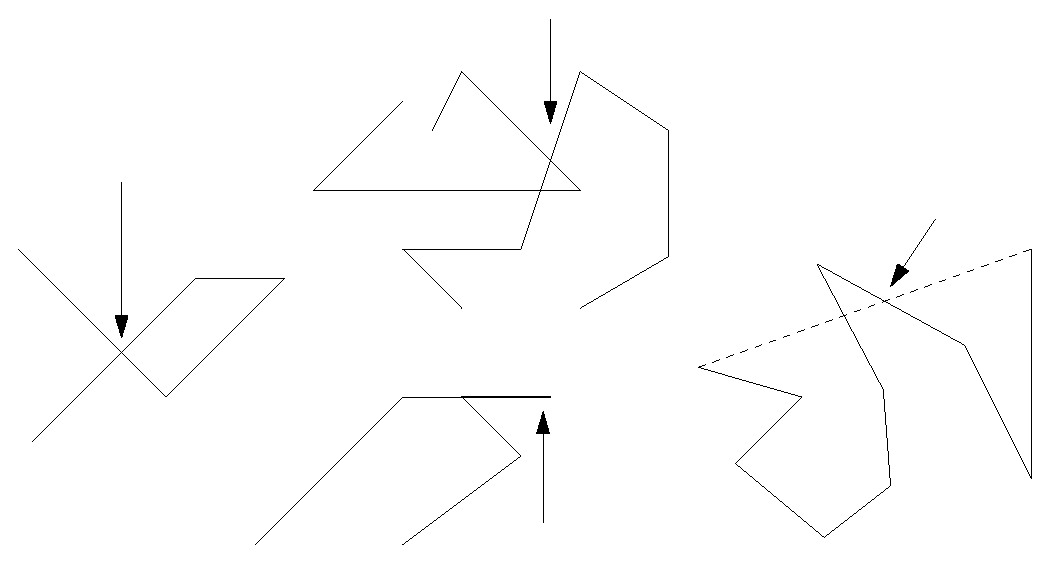
\includegraphics[width=.45\textwidth]{divaproblems}
}\parbox{.5\textwidth}{\caption[Example of improper contours.]{Example of improper contours. Left: crossing of two segments of a same contour; up: crossing of two different contours; right: first and last points of the contour generate a segment that crosses the other parts; down: two contours having a common segment.\label{divaprob}}
}
\end{figure}

Remember that you can use the tool \texttt{divacck} for checking and thinning of contours.


\subsection{From topography\label{sec:contourtopo}}
%--------------------------------------------------


Once you have placed files \texttt{topo.grd} and \texttt{TopoInfo.dat} in directory \texttt{./input}, type \textcom{divacont} in the command line shell. This will generate several coastline files named \texttt{coast.cont.100nn}, where $nn$ corresponds to the $nn^{th}$ level defined in \texttt{contour.depth}. File \texttt{coast.cont} contains the coastline at the surface level ($z=0$).

As an illustration, we want to have contours from surface to a depth of \mbox{1000 m} every \mbox{200 m}, with \texttt{topo.grd} and \texttt{TopoInfo.dat} created in the Sec. \ref{sec:howtotopo}. To this end we use the following file:

\begin{exfile}[htpb]
\begin{footnotesize}
\begin{verbatim}
2500
2000
1500
1000
500
0
\end{verbatim}
\end{footnotesize}
\caption{contour.depth\label{contourdepth}}
\end{exfile}

Contours for the specified depths are showed on Fig. \ref{fig:contourdepth}.


\begin{figure}[htpb]
\centering
%\begin{tabular}{ccc}
\includegraphics[width=.33\textwidth]{Ghir_contour_0}\includegraphics[width=.33\textwidth]{Ghir_contour_500}\includegraphics[width=.33\textwidth]{Ghir_contour_1000}\\
\includegraphics[width=.33\textwidth]{Ghir_contour_1500}\includegraphics[width=.33\textwidth]{Ghir_contour_2000}\includegraphics[width=.33\textwidth]{Ghir_contour_2500}

\caption{Contour generated every 500 m from surface to -2500 m.\label{fig:contourdepth}}
\end{figure}

\subsection{Using ODV}
%---------------------

Tool \texttt{divacoa2cont} allows converting ODV-format coastlines to \diva-format coastlines. Simply copy coastline file in the \texttt{input} directory with the name \texttt{coast.coa} along with a \texttt{param.par} file and type \texttt{divacoa2cont} in the shell. 

This provides you the new file \texttt{./input/coast.cont}.



\subsection{From a mask}
%--------------------------

Simply look at \texttt{contourgen.f} and create the mask as you wish. Alternatively you can
create a pseudo-topography with adequate pseudo-depth at which you draw the contour.


%---------------------------------------------
\section{Determination of analysis parameters}
%---------------------------------------------

Two key parameters have to be adjusted before running an analysis: the correlation length ($L$) and the signal-to-noise ratio ($\snr$). Several tools are provided in order to help the user for the determination of these parameters.


\subsection{\texttt{divafit} \label{sec:divafit}}
%------------------------------------------------

The script \texttt{divafit}: uses the data (\texttt{./input/data.dat}) for a direct fitting of the covariance function (see Sec. \ref{sec:kernel}). Note that the fit needs a sufficiently large data set.

\subsubsection{Command description}
%-----------------------------------------

\texttt{divafit} \qquad: performs a fit of the data correlation function based on the whole data set. \\
\texttt{divafit -r} \qquad: puts the new value of $L$ in \texttt{param.par} in function of the fit.\\
\texttt{divafit n} \qquad: performs the fit on a sample of \texttt{n*(n-1)/2} couples of data (sub-sampling). 

\examples:\\
\texttt{divafit -r 100}: performs a fit on $4950$ couples of data and update the file \texttt{param.par}.

\btips
When dealing with very large datasets, using \texttt{divafit} with sub-sampling may save you a large amount of time.
\etips

\textbf{Note:} when using advection constraint and variable $L$, \texttt{divafit} will not provide a very meaningful value.

\subsubsection{Output files}
%---------------------------

In output file \texttt{./output/paramfit.dat}, the best estimates are given and could be used as parameter values for running \diva.
Estimates of the correlation length are rather robust while those of the signal-to-noise ratio are neither precise nor robust, especially for large values.

Output file \texttt{covariance.dat} is the data-based covariance function (column 1: distance between points, columns 2: covariance, column 3: number of data couples used to estimate the covariance). 

Output file \texttt{covariancefit.dat} allows looking at the fitted covariance function (column 1: distance between points, 
column 2: data-covariance, column 3: fitted covariance).

Finally, file \texttt{param.par.fit} is the original param.par file except that the correlation length has been replaced by the fitted value. 

\textbf{Note:} always have a look at the fit to judge on its quality. %see example ref... divacovafit

\subsection{\texttt{divagcv}}
%-------------------------------

The script \texttt{divagcv} exploits \diva\, module (\texttt{gcvfac}), analyzing random fields to assess the generalized cross validator (GCV, see Chap. \ref{gcv} for theoretical developments). The script \texttt{divagcv} is an example of how to minimize the estimator by changing the signal-to-noise ratio ($\snr$) value, but could be adapted to optimize other parameters as well, such as correlation length.

Input to the module is the number of random estimates required (the larger the value, the more robust the estimator). Default value is 5, unless you change in \texttt{divacalc}. The user has to provide an input file \texttt{./input/gvcsampling.dat} containing the list of values for $\snr$ on which to try the estimator (typically around the values provided by \texttt{divafit}).

During the \texttt{divagcv} execution, error-field calculations are disabled to reduce computing time. 

\btips
If a mesh already exists (in \texttt{meshgenwork} directory), \texttt{divagcv} disables the \texttt{divamesh} procedure. For this reason, ensure you are working with the adequate mesh.
\etips





\subsubsection{Output files}
%---------------------------

File \texttt{./output/gcv.dat} contains the GCV estimator (column 1: S/N, column 2: GCV, column 3: data anomaly variance) and \texttt{./output/gcvsnvar.dat} the best new estimate for the S/N and \texttt{VARBAK} parameters.

In \texttt{param.par.gcv}, you find an adapted version of the original \texttt{param.par}.



\subsection{\texttt{divacv}}
%-------------------------------

\texttt{divacv} carries out a cross validation, point by point, without new matrix inversions. 

\subsection{\texttt{divacvrand}}
%-------------------------------

\texttt{divacv} runs a cross validation by sub-samples of points.


Note that in the present version (\diva-\divaversion), tools  \texttt{divacv} and \texttt{divacvrand}  
do not adapt the error norm to include the relative weights on data. This will be introduced in the next versions.



\section{Data selection tools (Version 1.0)}
%--------------------------------------------


This is a quick guide to use scripting tools to extract data from an ascii spreadsheet file compliant with the ODV-spreadsheet format (both full and compact version). The extracted data file can then directly be used as the input file ({\tt data.dat}) for \diva.

\subsection{Installation} 
%------------------------


Place yourself in a directory of you choice, typically {\tt diva-x.y.z}
\begin{itemize}
\item
 {\tt gunzip diva-selector.tar.gz}
 \item 
 {\tt tar -xvf diva-selector.tar} 
 \end{itemize}
This creates a directory {\tt ./selector} where you should perform the data extraction, so place yourself there ({\tt cd selector}). In this directory you find scripts {\tt divaselector} and {\tt divaguessforms}.

Use {\tt divaguessforms} on one of your ODV-spreadsheet files 
({\tt divaguess\-forms myODV\-spread\-sheet\-.txt})
to create a template {\tt select.form.guess} including
guesses on delimiters ({\tt ;} or {\tt TAB}), coordinates columns, depth columns, and date columns. Use this template to create your own forms {\tt select.form} by copying the template ({\tt cp select.form.guess select.form}).
Should you not use the ISO Date format, it can be adapted in {\tt diva\-selector} (head of the file) and {\tt diva\-guessforms} (tail of the file, look for {\tt yyyy}). To help you selection the columns, {\tt diva\-guessforms} creates a file {\tt ODVcolumns} with the title and number of each column interpreted from the input file.
 
\subsection{Batch use}
%---------------------

\begin{itemize}
\item Edit {\tt select.form} and {\tt timeselect.form} to adapt to your selection criteria.
\item Execute {\tt divaselector myODVspreadsheet.txt data.dat} to extract data based on the criteria and create a {\tt data.dat} suitable for input into \diva.
\end{itemize}

You can wrap these two steps into loops by dynamically creating {\tt select.form} (\textit{e.g.} for different depth values).

Note that {\tt divaselector} creates an {\tt awk} extraction program {\tt makeselection} that you can save under another name if you want to adapt it for further use (calculating data weights depending on depth for example).




\subsection{Form definition}
%---------------------------

The selection of fields is based in ascii file {\tt select.form}. 

In this example, longitude data are found in column 4 of the spreadsheet, latitude in column 5.
Weights and Date allow the column parameter to be zero (weights are then 1 and no date test will be performed respectively).

In detail, the file defines the structure of the input file and selection criteria
\begin{itemize}
\item
The first line contains the delimiter used in the file ($\backslash${\tt t} or {\tt ;})
\item 
The second line {\bf must} contain x coordinates information

{\tt free-name  column-in-data-file  xmin xmax}. 

Data will be taken if \texttt{x} values are in the range \texttt{xmin-xmax}. If \texttt{xmin=*}, no test on \texttt{xmin} will be performed (\textit{i.e.} all values lower than \texttt{xmax} are taken). Similarly, if \texttt{xmax=*}, no test on \texttt{xmax} is performed.

\item On the obligatory third line, we have a similar structure for the y coordinate
 
{\tt free-name  column-in-data-file  ymin ymax}

\item In the fourth line the variable to be analysed, is specified, with the same structure .

\end{itemize}


These four lines are mandatory.


\begin{itemize}
\item

A fifth line can contain the relative data weights

{\tt free-name  column-in-data-file  wmin wmax}

In addition, if {\tt column-in-data-file} is zero, then relative data weight are taken 1 (and the two last parameters are without effect)

\item The sixth line is related to time-selection and only two parameters are actually used
{\tt free-name column-in-data-file}

Because of the special pattern of time, range in time is not specified by min-max values
but in a separate file {\tt timeselect.form}. 
If {\tt column-in-data-file} for the time-selection is zero, no selection on dates is performed and all data satisfying the other criteria will be taken. 

\item 
Any additional line of {\tt select.form} after the sixth will add selection criteria with the same structure

{\tt free-name column-in-data-file minval maxval}

\end{itemize}


The addition criteria can be used to select depth ranges for example or water masses (salinity and temperature in given ranges). They can also be used to select data corresponding to quality flag values.

In the example {\tt select.form}, temperature data will be extracted west of $-10.4$ degrees longitude, with depth
of data between 20 and 30.5 meters and salinity values below 39.

The file {\tt timeselect.form} has a similar form than the {\tt select.form} but is only dealing with the allowed
ranges for years, month, days, hours and minutes (the columns position is defined in {\tt select.form}).
The selection is done as for {\tt select.form} with {\tt *} standing for no test. 
In the example, all data from year 1960 on are taken whenever they correspond to October, November or December.

\subsection{Tricks}
%------------------

\begin{itemize}
\item If you have several ascii input files with different structures, you can create a selection (with wild cards) for each of them that leads to an identical output structure. Then you can concatenate ({\tt cat}) these output files into a singly coherent
file.

\item If you have a very large data file, instead of running {\tt divaguessforms} on this file, first create a smaller one {\tt head -1000 myfile > testfile} and apply {\tt divaguessforms testfile}.

\item If the spreadheet file is created by an export from ODV, quality flags generally follow the variable to which they correspond. Hence if on the fourth line (variable to analyse) of {\tt select.form} you specify column 12 for example, on line seven of {\tt select.form} you can include 

{\tt qualityflag  13   3 3}

to select all data with quality flag value 3.

\item If you just need a few data extractions and prefer a graphical interface, import the data into ODV. Then use the
{\tt Configuration -> Selection criteria}, make your selection, go into {\tt SURFACE} (or {\tt SECTION}) mode and use the {\tt Export X/Y/Z} tool that produces a {\tt win1.oai} file almost ready for \diva\, input as {\tt data.dat}. You only need to adapt the fourth column so that it includes ones, nothing or relative weights. You can achieve this for example on a command line with {\tt awk '\{print \$1,\$2,\$3,1\}' win1.oai > data.dat}
\end{itemize}

{\bf Note:} The extraction for large data sets with {\tt divaselector} can be time consuming since it is based on non-optimized {\tt awk} coding.
 
\begin{exfile}[H]
\begin{footnotesize}
\texttt{
$\backslash$ t\\
Longitude  4  -10.4  *\\
Latitude  5  *  *\\
Temperature  10  *  *\\
Weights   0   1    1\\
Date  6  \\
Depth  8  20  30.5\\
Salinity  12  *  39\\
}
\end{footnotesize}
\caption{{\tt select.form} file content.} 
\end{exfile}


\begin{exfile}[H]
\begin{footnotesize}
\texttt{
year 1960 *\\
month 10 12\\
day * *\\
hour 0 24\\
min 0 60
}
\end{footnotesize}
\caption{{\tt timeselect.form} file content.} 
\end{exfile}





%---------------------------------------------

\section{Misc}
%--------------

\subsection{\texttt{divaclean}}
%-----------------------------

\texttt{divaclean} cleans up the working directories by removing \texttt{fort.*} files from \texttt{divawork} and \texttt{meshgenwork}, as well as output files from \texttt{output}.

\subsection{\texttt{divadataclean}}
%-----------------------------

Script \texttt{divadataclean} takes the input data \texttt{./input/data.dat} and eliminates all data that fall outside the bounding box of the contours (\textit{i.e.} the rectangle containing the analysis mesh). This avoids loading unnecessary large input files. If two additional arguments $n_{1}$ $n_{2}$ are added, data values falling outside the range specified by $n_{1},n_{2}$ are also eliminated.

\example\\
\texttt{divadataclean -3 35} \qquad \begin{minipage}[t]{.65\textwidth}removes all data points of which the value is not between $-3$ and $35$.\end{minipage} 

The output overwrites \texttt{./input/data.dat} but keeps the original one in \texttt{./\-input/\-data\-.dat\-.full}. The tool should be used just after having loaded the data set (typically after \texttt{divaload}).

\subsection{\texttt{divaload}\label{sec:divaload}}
%--------------------------------------------------

\texttt{divaload} loads input files from the chosen directory into \texttt{divastripped/input/}. You just have to specify the directory where your input files are located (relative or absolute paths). It is assumed that the input files are located in a folder \texttt{input} within the chosen directory.\\
\examples\\
\textcom{divaload ./AdriaticTemperature} will load the files from\\
 \texttt{./\-Adriatic\-Temperature/\-input}
 
\textcom{divaload c:/data/AdriaticTemperature} will load the files from\\
\texttt{c:/\-data/\-Adriatic\-Temperature/\-input}

\btips
When you want to know to which correspond the data present in the input directory, simply read the content of the file \texttt{input/casename}; it indicates the repertory from which you loaded input files with command \texttt{divaload}.
\etips


\subsection{\texttt{divacck}}
%-----------------------------

\texttt{divacck} checks your initial contour file \texttt{./output/coast.cont}. In output \texttt{./\-output/\-coast.cont\-.checked} you will find a thinned contour based on the length scale, where the possible couples of identical points are eliminated.

Application of \texttt{divacck} is normally not necessary if you created the contours with \texttt{divacont}.

% DivaPreprocessing
\chapter{Running analysis \label{chap:running}}

Once all the input files are prepared, you are ready to create analysed gridded fields. The whole procedure is described in the present chapter.

\minitoc

\section{Running a simple analysis}
%----------------------------------


\subsection{\command{divadress}}
%-----------------------------

The simplest procedure to carry out an analysis with \diva is using the command \command{divadress}, which performs the four following operations:

\begin{enumerate}
\item \command{divaclean}
\item \command{divamesh}
\item \command{divacalc}
\item \command{divaqcbis}
\end{enumerate}

\subsection{\command{divamesh}}
%-----------------------------

\index{Finite-elements}
\index{Mesh}
Generates the finite-element mesh based on contour(s) specified in file \file{coast.cont} and correlation length provided in \file{param.par}; remember that the correlation length shall have an appropriate value in order to obtain a correct mesh:
\begin{itemize}
\item Contour segments should not be much smaller than finite element length; if your contour is too fine, the tool \command{divacck} can be used in order to reduce the contour resolution.
\item The typical length of a finite element should be smaller than the correlation length, otherwise the grid would be too coarse compared to the signal to resolve.
\end{itemize}


\begin{figure}[htpb]
\centering
\parbox{.7\textwidth}{
\includegraphics[width=.65\textwidth]{island_mesh}
}\parbox{.3\textwidth}{
\caption{Mesh on a simple domain.}
}
\end{figure}

Note that since version \diva-\divaversion, mesh generation takes into account coordinate change (specified by \texttt{icoord}) so that meshes are uniform in the transformed domain. 


\subsubsection{Mesh with different element sizes}

You also have the possibility to create of mesh of which the size of the elements varies over the domain. To this aim, you have to create a \textit{mesh density} file that indicates what length scale has to be applied in a determined region. This file is named \file{coast.cont.dens} and has to be placed in \directory{divastripped/input/}.

We considered the simple island case, of which the contour file given by

\begin{exfile}[htpb]
\begin{footnotesize}
\begin{verbatim}
2
4
0	0
5	0
5	5
0	5
4
2	2
2	3
3	3
3 2
\end{verbatim}
\end{footnotesize}
\caption{coast.cont}
\end{exfile}

We choose a value of $2.5$ for the global mesh (specified in \file{param.par}) and define a finer mesh around the island through the following \file{coast.cont.dens} file:

\begin{exfile}[htpb]
\begin{footnotesize}
\begin{verbatim}
1
0.125 4
1 1
4 1
4 4
1 4
\end{verbatim}
\end{footnotesize}
\caption{coast.cont.dens}
\end{exfile}

which means that we want a length scale of 0.125 in the domain defined by by the four points (1 1), (4 1), (4 4), (1 4). Be sure that the domain where you want to have a finer mesh is on the left when following the contour. The mesh generated with these conditions is presented on Fig.~\ref{fig:square}.

\begin{figure}[htpb]
\centering
\includegraphics[width=.75\textwidth]{finer_mesh}
\caption{Mesh refinement around the island.\label{fig:square}}
\end{figure}



\subsection{\command{divacalc}\label{sec:divacalc}}
%-----------------------------

\command{divacalc} is the script that runs the analysis by solving the variational principle over the domain of interest. To work properly, it needs a data file, a parameter file, and a finite-element mesh.

\btips
As the mesh generation is often the most time-consuming part of a \diva execution, remember that once you have created the mesh, you do need to run \command{divadress} each time you want a new analysis, but just \command{divacalc}.
\etips

\begin{figure}[H]
\centering
\parbox{.7\textwidth}{
\includegraphics[width=.65\textwidth]{island_analysis}
}\parbox{.3\textwidth}{
\caption{Example of analysed field.}
}
\end{figure}


\subsubsection{Output files}
% -------------------------

\begin{itemize}
\item \file{fieldgher.anl} and \file{errorfieldgher.anl} are respectively the analysis and the error fields (in \texttt{gher} format) on the regular grid specified in \file{param.par};
\item \file{fieldascii.anl} and \file{errorfieldascii.anl} are the same as \file{fieldgher.anl} and \file{errorfieldgher.anl}, but in \texttt{ascii} format;
\item \file{valatxyascii.anl} and \file{erroratxyascii.anl} give respectively the values of the analysis and the error fields at the points specified in file \file{valatxy.coord};
\item \file{fieldatdatapoint.anl} and \file{erroratdatapoint.anl} are respectively the analysis and error fields computed at the data points (\textit{i.e.} the points from \file{data.dat});
\item \file{results.nc} (located in \directory{./output/ghertonetcdf}) is a NetCDF \index{NetCDF} file containing the gridded analysis and error fields (provided error calculation is switched on).
\end{itemize}


\section{Quality control of data}
%--------------------------------

\index{Quality control}
According to theoretical developments of Chapter~\ref{chap:analysisparameters}, quality control with \diva can be performed using to one of the three criteria \eqref{eq:qc1}, \eqref{eq:qc2} or \eqref{eq:qc3}, respectively implemented in \diva with \command{diva\-qc}, \command{diva\-qc\-bis} and \command{diva\-qc\-ter}. 



\subsection{Tools}

There are three tools to perform QC:
\begin{description}
\item[\command{divaqc}:] it is the most expensive version of QC, since $A_{ii}$ must be evaluated by analysis of vectors with zeros everywhere, except at the $i^{th}$ position.
\item[\command{divaqcbis}:] this version of the QC is quicker, as we replace $A_{ii}$ by its average $\frac{1}{N}\trace{\matr{A}}$.
\item[\command{divaqcter}:] the last criterion implemented is based on the RMS value of the misfit and the generalized cross validator $\Theta$. 
\end{description}

\subsection{Output files}

The corresponding outputs are given in \file{out\-liers.dat}, \file{out\-liers\-bis.dat} and \file{out\-liers\-ter.dat}.
The modules \command{divaqc*} also generate \file{outliers*.normalized.dat}, which contain, in a sorted way (from the most suspect data to less suspect), the possible outliers from the normalized misfits test \eqref{eq:qc4}.

\btips
By default, the criterion used in \command{divadress} is \command{divaqcbis}, but you can change it by editing the file \command{divadress} and replacing \command{divaqcbis} by one of the other quality test (\command{divaqc} or \command{divaqcter}).
\etips


\section{Running a semi-normed analysis}
%---------------------------------------

\index{Semi-normed analysis}
A semi-normed analysis consists of four steps:
\begin{enumerate}
\item create a so-called \textit{reference field}, which will act as background field (Section~\ref{sec:gridding});
\item subtract the reference field from the data values in order to work with anomalies;
\item perform an analysis on the anomalies;
\item reconstruct the field by adding the analysed anomaly field to the background (reference) field.
\end{enumerate}

These four steps are executed by running script \command{divaseminorm} and the implemented tools described hereinafter. Note that the parameters written in the original \file{param.par} file will be used during the analysis on the anomalies. Thus it is advised to specify \texttt{ireg}=0, so that no background field will be subtracted from the anomaly. 

\subsection{\command{divarefe}}
%-----------------------------

This script performs an analysis on your original data, but modify the analysis parameters: $L$ is multiplied by $5$ and $\snr$ by $0.1$. 

\subsubsection{Output files}
%---------------------------

They are the same as those created through an execution of \command{divacalc}, but assigned with a suffix \file{.ref}:
\file{fieldgher.anl.ref}, \file{fieldascii.anl.ref}, \file{valatxyascii.anl.ref} and \file{fieldatdatapoint.anl.ref}.


\subsection{\command{divaanom}}
%-----------------------------

The script use file \file{fieldatdatapoint.anl.ref} to compute the difference between data and analysed (reference) field to obtain anomalies.

\subsubsection{Output files}
%---------------------------

File \file{data.dat} contains anomalies instead of the original data, while file \file{data.dat.full} is the copy of your original data file.


\subsection{\command{divacalc}}
%-----------------------------

This command was previously described (Section~\ref{sec:divacalc}). The only difference is that it is applied here on anomalies.


\subsection{\command{divasumup}}
%-----------------------------

\command{divasumup} performs the last step of a semi-normed analysis: the sum of background field and analysed anomaly field. 

\subsubsection{Output files}
%---------------------------

They are the same as those created through an execution of \command{divacalc}. Note that after an execution of \command{divasumup}, \file{data.dat} contains the original data, while \file{data.dat.anom} contains the previously computed anomalies. 



\section{Extras}
%---------------

\subsection{Saving outputs}
%--------------------------

\command{divasave} is designed for saving the outputs in the folder \directory{output} to the chosen directory.

\example
\begin{lstlisting}[style=Bash]
[charles@gher13 divastripped] divasave ~/DIVA/test/
\end{lstlisting}
will save the files into \directory{\textasciitilde/DIVA/test/}

\subsection{Checking of installation}
%------------------------------------

\command{divacheck} makes the comparison of analysis results with reference analysis (for
installation check, compiler option testing or checking of new versions)

%-------------------------------------------------------------------------------------------


\section{Analysis with advection constraint activated\label{sec:advection}}
%---------------------------------------------------

\index{Advection}
The input files needed for such analysis are the same as for a basic analysis, except that you need to provide a velocity (or pseudo-velocity) field, specified through the following files:
\begin{itemize}
\item \file{Uvel.dat} and \file{Vvel.dat}, which contain the two components of the velocity. They have the same format (binary) as \file{fieldgher.anl}. An example of generation of such files is in the test case {\tt advectiontest}.
\item \file{UVinfo.dat}, which specifies the grid on which the velocity field is defined. It has the same format as \file{GridInfo.dat} or \file{TopoInfo.dat}).
\item \file{constraint.dat}, which activates the advection constraint and contains parameters $\theta$ and $\mathcal{A}$. Refer to Chapter~\ref{chap:advection} for theoretical details.
\end{itemize}

\begin{exfile}[htpb]
\begin{footnotesize}
\texttt{
-3.\\
-3.\\
0.100000001\\
0.100000001\\
61\\
61
} 
\end{footnotesize}
\caption{UVinfo.dat\label{ex:UVinfo.dat}}
\end{exfile}


\begin{exfile}[htpb]
\begin{footnotesize}
\texttt{
100 0.0
} 
\end{footnotesize}
\caption{constraint.dat\label{ex:constraint.dat}}
\end{exfile}

%Instead of reading in nodal properties, directly read in a gridded field 
%for $u,v$.
%Example on coordinate change effect
%In other words, (yes for velocity, but check for diffusion}, formulation 
%is done in cartesian coordinates (or any other unchanged coordinates). 
%For convenience \texttt{icoord=1} transforms input data (data location 
%and contour location) into cartesian grid, but diffusion coefficient 
%must be taken care of (if data in degrees and \texttt{icoord=1}, must be provided 
%in $m^2/s$ when velocities are in $m/s$)

%\paragraph{Files manupilated by advection constraint:}

% or matlab file {\tt } (TO BE created).


\subsection{Interplay with coordinate change on}
%--------------------------------------------------

In this example, we work on a region $[-1,1]\, \times\, [59,61]$ with $L=0.2$ and $\lambda=1$.
 
With no coordinate change (i.e., \texttt{icoordchange=0} in \file{param.par}), coordinates are taken as such and
a single point in the center leads to an analysis that is circular when axes on $x$ and $y$ are drawn with equal scales (Fig.~\ref{fig:nocoord}).

\begin{figure}[H]
\centering
\includegraphics[width=.75\textwidth]{nocoord}
\caption{Analysis without coordinate change.\label{fig:nocoord}}
\end{figure}


On the other hand, if coordinate change is \textsl{on} (i.e., \texttt{icoordchange=1} in \file{param.par}), the analysis is isotropic in the real space.

At $60^{\circ}$ North, a degree E-W covers half the real distance of a degree S-N. On a graph scaled so that $x$ and $y$ are distances, the analysis is again isotropic (this is the desired effect). If you plot the same analysis with $x$ and $y$ axes equally spaced in degrees (as for the previous case), you will obviously get an ellipse (Fig.~\ref{fig:coord}, left).

\begin{figure}[H]
\centering
\begin{tabular}{cc}
\raisebox{.2\textwidth}{\includegraphics[width=.4\textwidth]{coord}}& \includegraphics[width=.4\textwidth,height=.8\textwidth]{coord}\\
\end{tabular}
\caption[Analysis with coordinate change.]{Analysis with coordinate change: the two figures represent the same field, but are drawn with different scales for the axes.\label{fig:coord}}
\end{figure}


If we add an advection constraint characterized by $u=v=1 (m/s)$, the case with no coordinate change leads to a signal along the bisector (Fig.~\ref{fig:constrnocoord}).


\begin{figure}[H]
\centering
\parbox{.6\textwidth}{
\includegraphics[width=.55\textwidth]{constrnocoord}
}\parbox{.4\textwidth}{
\caption{Analysis with advection but without coordinate change.\label{fig:constrnocoord}}
}
\end{figure}


If coordinate change is activated, the advection direction in real space is not any more along the bisector in degrees, but in km (Fig.~\ref{fig:constrdegrees}). Note that the advection constraint scales the overall velocity, so that a coordinate change does not change the intensity of the advection constraint, but only its direction.


\begin{figure}[H]
\centering
\begin{tabular}{cc}
\raisebox{.2\textwidth}{\includegraphics[width=.4\textwidth]{constrdegrees}}&\includegraphics[width=.4\textwidth,height=.8\textwidth]{constrdegrees}
\end{tabular}
\caption{Analysis with advection and coordinate change.\label{fig:constrdegrees}}
\end{figure}




\begin{figure}[H]
\centering
\includegraphics[width=7cm,height=14cm]{advdiffcoord}
\caption{.}
\end{figure}


Note that the diffusion coefficient is not changed. If this coefficient is given in 
Cartesian coordinates (in this case, it must be specified in $m^2/s$ if 
velocities are in $m/s$) but you provide input in degrees and do not set 
\texttt{icoord=1}, the diffusion coefficient is basically overestimated by a 
factor $10^5$.


For example, in the grid with \texttt{icoord=0} we can activate diffusion

\begin{figure}[H]
\centering
\includegraphics[width=7cm,height=14cm]{advdiffnocoord}
\caption{Diffusion coefficient divided by 110000 compared to the 
\texttt{icoord=1} case.}
\end{figure}


With no coordinate change, input values are taken as is. To recover a similar (but tilded and boundary modified) solution, we have to change manually the coefficient and divide by $110000$ (degrees to meter scaling) so that the actual Reynolds number remains the same.

%--------------------------------------------------------------------------------------------------------

\section{Summary: typical execution chains}
%------------------------------------------


\subsection{Simple analysis}
%---------------------------

It is assumed that all the input files are already prepared and the parameters correctly assigned.

\begin{enumerate}
\item \command{divaload} your\_directory
\item \command{divadress}
\item \command{divasave} your\_directory
\end{enumerate}



\subsection{Analysis with evaluation of parameters}
%--------------------------------------------------

You start with correct data and contour file, but with parameters file that needs to be adapted.

\begin{enumerate}
\item \command{divaload your\_directory}
\item \command{divafit -r} \qquad to compute the correlation length and replace its value in \file{param.par};
\item \command{divagcv -r} \qquad to compute the signal-to-noise ration and variance of the background field, and replace them in \file{param.par};
\item \command{divadress}
\item \command{divasave your\_directory}
\end{enumerate}


% to add sth

\chapter{Postprocessing tools\label{chap:postprocessing}}

Various tools are available for visualization and processing of the gridded fields; some of them are presented in the following sections. It is up to the user to utilize his favourite drawing tools for representing the numerical results. Nevertheless, we provide several basic tools easily adaptable to facilitate the task.


\minitoc

\section{Gnuplot\label{sec:visugnuplot}}
%-------------------------------------------

\index{Gnuplot}
\textsl{Gnuplot} is a free portable command-line driven interactive data and function plotting utility, available for various platforms (\url{http://www.gnuplot.info/}). We provide some routines for plotting \diva inputs and outputs (data, contour, mesh, analysis etc) with the help of this tool. Running \command{divagnu} makes plots in \texttt{png} format. 

\begin{tips}
Plots provided by \gnuplot are made to help the user to have a quick look at the results, immediately after the execution. However, these plots are not always suitable for publications or diffusion. The user is invited to create his own post-processing tools based on the examples provided in the next sections.\end{tips}

\begin{tips}
If you need larger fonts, on some systems they are available and you can edit the plotting program \file{gnuwork$\backslash$divaplotall}
and replace the driver definition by
\begin{tiny}
\begin{verbatim}
echo set terminal png transparent giant font system 14 size 1920,1540 crop \#ffffff >> bidon
\end{verbatim}
\end{tiny}
\end{tips}

\begin{tips}
If you do not need all plots but only a few (eg. analysis, error and coastline) of them you can edit the plotting program \file{gnuwork$\backslash$divaplotall} and replace the script line \verb#for i in `ls diva_*`# 

by
\end{tips}

\verb#for i in diva_analysis diva_error diva_coastline#

\subsection{Installation}
%---------------------------

\gnuplot can be easily downloaded for windows systems on the web page \url{http://www.gnuplot.info}. For Cygwin users, there are two possibilities:

\begin{enumerate}

\item you do not have X Windows System installed: in this case, it is advised to only install \texttt{wgnuplot}, available at\\
\url{http://downloads.sourceforge.net/gnuplot/gp422win32.zip} for version 4.22.\\
Once you have downloaded it, just unzip the folder in the location of your choice (provided it is located on the path of your system). The \gnuplot\, window is activated either by typing \command{wgnuplot} in the Cygwin shell, or by creating a short-cut on your desktop to the executable \texttt{wgnuplot.exe}


\begin{figure}[htpb]
\centering
\parbox{.6\textwidth}{
\includegraphics[width=.55\textwidth]{gnuplotwindows}
}\parbox{.4\textwidth}{
\caption{Gnuplot window.\label{fig:gnuplotwindows}}
}
\end{figure}

\item X Windows System is already installed: run again the Cygwin \command{setup.exe} (for downloading and updating your Cygwin installation); in the "Select Packages" screen, look for the "Math" entry, select \gnuplot\, and choose "`install". Once this installation is finished, \gnuplot\, is launched from a XWin (obtained after typing \texttt{startx}) window by typing \texttt{gnuplot}.

\begin{figure}[htpb]
\centering
\parbox{.7\textwidth}{
\includegraphics[width=.65\textwidth]{gnuplotinstall}
}\parbox{.3\textwidth}{
\caption{Installing \gnuplot\, with cygwin.\label{fig:gnuplotinstall}}
}
\end{figure}

\end{enumerate} 


\subsection{Utilization}
%-------------------------


Normally Fortran sources (\file{forgnuplot*.f}) have been compiled during the \diva installation and executables placed into \directory{DIVA3D/bin/}.

In directory \directory{divastripped/gnuwork/}, edit \command{divaplotall}  and adapt the header so that  \texttt{gplot} indicates the correct path to your \gnuplot executable.

\example\\
\begin{verbatim}
#====================================================
# ADAPT the following to the gnuplot executable
gplot=/cygdrive/c/cygwin/usr/gnuplot/bin/wgnuplot.exe
#====================================================
\end{verbatim}

From \directory{divastripped}, after running an analysis, type \command{divagnu}: this will create the figures in directory \directory{gnuwork/plots/}.
Note that \command{divagnu} will try to create all the possible figures, even if the corresponding script was not run, e.g., plot of outliers when no outlier detection was performed. This is why so many error messages are written on the screen, but you do not have to take them into account.
 %necessary for the plot inside the directory \texttt{./divastripped/gnuwork}

%From within gnuplot (Fig. \ref{fig:gnuplotwindows}): place yourself in the \texttt{gnuwork} directory and type:
%\begin{listevide}
%\item load 'gnuplotdata'
%\item load 'gnuplotcoast'
%\item load 'gnuplotcoastfilled'
%\item load 'gnuplotmesh' (mesh as triangles)
%\item load 'gnuplotmeshl'  (mesh with lines)
%\item load 'gnuplotanalysis'
%\item load 'gnuplotanalysissmooth'
%\item load 'gnuploterrorfield'
%\item load 'gnuplotuv'
%\end{listevide}
%
%These commands allow you to have a quick look at your data and results. In the file \texttt{gnuplotdata}, you might need to play with the value following the \texttt{ps} command (device dependent). 

Here are some examples of plots created with \gnuplot:

\begin{figure}[htpb]
\centering
\subfigure[Data and coastline]{
\includegraphics[width=.30\textwidth,height=.30\textwidth]{gnuplot_data_coast}
}\subfigure[Filled coastline]{
\includegraphics[width=.30\textwidth,height=.30\textwidth]{gnuplot_coastlinefilled}
}\subfigure[Mesh]{
\includegraphics[width=.30\textwidth,height=.30\textwidth]{gnuplot_mesh}
}

\subfigure[Numbered mesh]{
\includegraphics[width=.30\textwidth,height=.30\textwidth]{gnuplot_mesh_numbered}
}\subfigure[Analysis]{
\includegraphics[width=.30\textwidth,height=.30\textwidth]{gnuplot_analysis}
}\subfigure[Error and data locations]{
\includegraphics[width=.30\textwidth,height=.30\textwidth]{gnuplot_error_data}
}
\caption{Visualization with \gnuplot.\label{fig:gnuplotexamples}}
\end{figure}


\section{\matlab / Octave}
%-------------------

%http://modb.oce.ulg.ac.be/mediawiki/index.php/NetCDF_toolbox_for_Octave

\index{Matlab}
Tools to display contours, data, meshes, analysis and error fields are available at \url{http://modb.oce.ulg.ac.be/mediawiki/index.php/Diva_matlab}. 

\subsection{Installation}

Download and extract the archives \file{Diva\_matlab.tar.gz} and \file{matlab\_example.tar.gz}
\begin{lstlisting}[style=Bash]
 tar -xvf Diva_matlab.tar.gz
 tar -xvf Diva_matlab_example.tar.gz
\end{lstlisting}

In order to have the routines working properly, you need to install:
\begin{description}
\item[NetCDF toolbox,] for reading the result files. For recent versions of \matlab, the routines for reading/writing NetCDF are readily available. For older versions, you can install it from \url{http://mexcdf.sourceforge.net/downloads/}.
\item[m\_map toolbox:] optional but recommended, it allows one to plot generate various plots (mesh, data, analysis) using coastlines, projections etc (\url{http://www.eos.ubc.ca/~rich/map.html}). 
\end{description}
    

\subsection{Tools description}
%--------------------------
 
\begin{table}[htpb]
\centering
\caption[\matlab programs for plotting.]{\matlab programs for plotting. Set \texttt{mmapflag}=1 if the m\_map toolbox is installed. \texttt{valex} stands for exclusion value.}
\begin{tabular*}{\textwidth}{@{\extracolsep{\fill}}llll}
\toprule
Routine				&	Mandatory input(s) 		&	Optional input(s)	& 	Utility  			\\
\midrule
diva\_contour.m 		&	contourfile 			& mmapflag 			&	Plot contour		\\
diva\_mesh.m 			& meshfile, meshtopofile 	& mmapflag 			&	Plot mesh			\\
diva\_data\_positions.m	& datafile 					& dotsize, mmapflag & 	Plot data locations	\\
diva\_data.m 			& datafile 					& dotsize, mmapflag & Plot data values		\\
diva\_analysis.m 		& resultfile 				& valex, mmapflag 	 & Plot the analyzed field \\
\bottomrule
\end{tabular*}
\end{table}

\subsection{Examples of use}
%------------------------------------------------------------

Open a \matlab session and set the path to the directory containing the function:

\begin{lstlisting}[style=Matlab]
addpath('path_to_functions')
\end{lstlisting}

Define the input files:

\begin{lstlisting}[style=Matlab]
exampledir   = path_to_example_directory;
contourfile  = [exampledir,'/coast.cont'];
datafile     = [exampledir,'/data.dat'];
meshfile     = [exampledir,'/mesh.dat'];
meshtopofile = [exampledir,'/meshtopo.dat'];
resultfile   = [exampledir,'/results.nc'];
\end{lstlisting}


Execute the different commands:
\begin{itemize}
\item Plot the contour:
\begin{lstlisting}[style=Matlab]
diva_contour(contourfile);
\end{lstlisting}

\item Plot the finite-element mesh:
\begin{lstlisting}[style=Matlab]
diva_mesh(meshtopofile,meshfile);
\end{lstlisting}


\item Plot the data positions:
\begin{lstlisting}[style=Matlab]
diva_data_positions(datafile);
\end{lstlisting}

\item Plot the data (with values):
\begin{lstlisting}[style=Matlab]
diva_data(datafile);
colorbar;
\end{lstlisting}

\item Plot the analysis:
\begin{lstlisting}[style=Matlab]
diva_analysis(resultfile);
colorbar;
\end{lstlisting}


\end{itemize}



The resulting figures (without the m\_map option) are shown below.

\begin{figure}[H]
\centering
\subfigure[Data]{
\includegraphics[width=.495\textwidth]{Diva_example_contour}
}\subfigure[Mesh]{
\includegraphics[width=.495\textwidth]{Diva_example_mesh}
}
\subfigure[Analysis]{
\includegraphics[width=.495\textwidth]{Diva_example_contour_data2}
}\subfigure[Outliers]{
\includegraphics[width=.495\textwidth]{Diva_example_analysis}
}
\caption{Examples of figures created with \diva-\matlab toolbox.}
\end{figure}



\section{Python}
%_--------------

Python (\url{http://www.python.org/}) is a object-oriented, free to use, programming language. It is directly available through the package manager of recent Linux distributions.

\subsection{Installation}

Download and extract the archive \file{Diva\_Python\_tools\_v1.0.tar.gz}
\begin{lstlisting}[style=Bash]
 tar -xvf Diva_Python_tools_v1.0.tar.gz
\end{lstlisting}

To have example files to test, extract the files from \file{matlab\_example.tar.gz} (the same files used in the previous section) inside the python directory:
\begin{lstlisting}[style=Bash]
ctroupin@gher13 cd Diva_Python_tools_v1.0
ctroupin@gher13 tar -xvf Diva_matlab_example.tar.gz
\end{lstlisting}

Along with Python, it is necessary to install:
\begin{description}
\item[NumPy] \url{www.numpy.org}, a package for scientific computing;
\item[SciPy] (\url{http://www.scipy.org/}), another package for science and engineering;
\item[matplotlib] (\url{http://matplotlib.org/}), a 2D plotting library, where one can find the basemap toolkit (https://pypi.python.org/pypi/basemap) particularly useful for plot data on map projection (somewhat equivalent to m\_map in Matlab).
\item[netcdf4-python] (\url{http://code.google.com/p/netcdf4-python/}), the Python/numpy interface to netCDF.
\end{description}

Under Linux, the first three items are available with the package manager. The NetCDF interface requires a manual installation.

\begin{itemize}
\item Download the archive from \url{http://code.google.com/p/netcdf4-python/downloads/list}
\item Check the \textit{sha1 sum} and extract the archive:
\begin{lstlisting}[style=Bash]
ctroupin@gher13 ~/Software $ sha1sum netCDF4-1.0.4.tar.gz 
cd1735a69446e558ba55034f184ee5f3d44d1a44  netCDF4-1.0.4.tar.gz
ctroupin@gher13 ~/Software $ tar -xvf netCDF4-1.0.4.tar.gz 
ctroupin@gher13 ~/Software $ cd netCDF4-1.0.4/
\end{lstlisting}
\item Follow the instruction written in file \file{README}:
\begin{lstlisting}[style=Bash]
ctroupin@gher13 ~/Software python setup.py build
ctroupin@gher13 ~/Software python setup.py install
\end{lstlisting}
\end{itemize}

\subsection{Usage}

Edit the files if necessary and run Python (either in a shell, or using a Python editor). An example of plots is shown in Fig.~\ref{fig:pythontoolbox}.

\begin{lstlisting}[style=Bash]
ctroupin@gher13 ~/ Diva_Python_tools_v1.0 python diva_plot_mesh.py
\end{lstlisting}

\begin{figure}[htpb]
\centering
\includegraphics[width=.495\textwidth,viewport=44 299 567 492]{contour_ex_py}\includegraphics[width=.495\textwidth,viewport=44 299 567 492]{mesh_ex_py}
\includegraphics[width=.495\textwidth,viewport=44 279 567 512]{data_ex_py}\includegraphics[width=.495\textwidth,viewport=44 279 567 512]{results_ex_py}
\caption{Examples of figures obtained with the \diva-Python toolbox.\label{fig:pythontoolbox}}
\end{figure}


\section[NetCDF visualization tools]{General NetCDF visualization tools}
%---------------------------------------------

NetCDF (network Common Data Form) format. It is an machine-independent format to represent scientific data. For more details, consult \url{http://www.unidata.ucar.edu/software/netcdf/}. \index{NetCDF}

There are several tools that aim to provide a quick view of the content of a NetCDF files, such as the analyse and error fields provided by \diva. It is possible to export the results as a figure, but generally these software do not offer the possibility to customize the plots as could be done with the previous tools.

\subsection{Ocean Data View}

\index{Ocean Data View}
Among the numerous possibilities offered by ODV, there is a tool for accessing and visualizing local or remote NetCDF files \citep[][Chapter~13]{SCHLITZER12}.



\subsection{NcBrowse}
%-------------------

\textsl{NcBrowse} is available at \url{http://www.epic.noaa.gov/java/ncBrowse/} and works with both Linux and Windows O.S.

\begin{figure}[htpb]
\centering
\includegraphics[width=.45\textwidth]{ncbrowse2}\hspace{.5cm} \includegraphics[width=.45\textwidth]{ncbrowse3} \\
\vspace{.5cm}
\includegraphics[width=.45\textwidth]{ncbrowse1} 
\caption{Plots of results with NcBrowse.}
\end{figure}

\subsection{Ncview}
%------------------

\index{Ncview}
\textsl{Ncview} (Linux and Windows + Cygwin) is available at\\
\url{http://meteora.ucsd.edu/~pierce/ncview_home_page.html}\\
but requires the NetCDF library to be compiled with your own system configuration.

\subsubsection{Installation under Linux}

Recent Linux distribution already permits the installation of Ncview through their package manager. Should it not be the case, the last version of Ncview is available here: \url{ftp://cirrus.ucsd.edu/pub/ncview/ncview-2.1.2.tar.gz}

\subsubsection{Installation under Windows-Cygwin}

Install and build the last NetCDF version for Unix: download the latest release and build as with Unix. The latest release is tested under Cygwin\index{Cygwin} and passes all tests cleanly. To build under Cygwin, follow the Unix build instructions in a Cygwin shell. The \texttt{--enable-shared} option to configure will generate the \file{netcdf.dll}. 


\begin{itemize}
\item Copy \url{http://www.unidata.ucar.edu/downloads/netcdf/netcdf-3_6_2/index.jsp}  into directory of your choice
\item Unzip the folder  and type:
\begin{lstlisting}[style=Bash]
[charles@gher13 Software]
./configure
...
make check..
...
make install
\end{lstlisting}

\item download \texttt{Ncview} and unzip the folder
\item type\\ 
\begin{lstlisting}[style=Bash]
[charles@gher13 Software]
./configure
...
make 
...
make install
\end{lstlisting}

\item type \texttt{startx} (check if you have installed \texttt{Xfree}) and in the newly opened window, type\\
\texttt{ncview name\_of\_the\_file.nc}

\item if the procedure is correctly followed, you should obtain windows similar to Fig.~\ref{fig:ncview}.
\end{itemize}

\begin{figure}[htpb]
\centering
\includegraphics[width=.45\textwidth]{ncview0}\hspace{.5cm} \includegraphics[width=.45\textwidth]{ncview1} \\
\vspace{.5cm}
\includegraphics[width=.45\textwidth]{ncview2} \caption{Plots of results with \textsl{Ncview}.\label{fig:ncview}}
\end{figure}

%DivaExamples
\chapter{Realistic examples\label{chap:examples}}

A few examples with real data are described in this chapter. They can act as model for users who need to perform such kind of analysis. 

\minitoc

\newpage

\section{Complete example}
%---------------------------------------------------

We present here a complete 2-D case treated in command-line. This example is taken from \citet{TROUPIN12}.

\subsection{Preparation of the input files\label{prep}}
%-----------------------------------------------------

To perform an analysis, you will need:
\begin{itemize}
\item a contour file (\file{coast.cont}),
\item a data file (\file{data.dat}), 
\item a list of run parameters (\file{param.par}) and 
\item the locations of the points where you want to know the value of the analysed field\\ 
	  (\file{valatxy.coord}).
\end{itemize}
Examples of these files are given in Chapter~\ref{chap:general}.

We recommend to create a new directory (let us call it \directory{case1}) for each case you will treat and within this directory, two sub-directories name input and output. The four input files are then placed in \directory{case1/input/}. 

Let us assume that you created \directory{case1} in \directory{\textasciitilde/Examples/}. To copy them into the \directory{diva\-stripped/\-input/} directory, use the command: 

\vspace{.25cm}
\begin{lstlisting}[style=Bash]
bash-3.2$ divaload ../case1
\end{lstlisting}
%$

\subsubsection{Data}

In this example we work with salinity measurements in the Mediterranean Sea at a depth of 30~m in September, for the 1980-1990 period (Fig.~\ref{fig:diva_oi_09_10030dataval_mesh3}). The data set is built up by exploiting the SeaDataNet portal (\url{http://www.seadatanet.org}) and the World Ocean Database 2009 \citep[WOD09,][]{BOYER09} and contains 1061 data points. 
% Notes: figures located /home/charles/DIVA/MedSea_PaperDIVA/figureOI/July1980_1990c/ps

\subsubsection{Parameters}

We start with the parameter file \ref{paramfileCL}: the regular grid for the analysis extends from 7$^{\circ}$W to 36$^{\circ}$E and from 30$^{\circ}$15'N to 45$^{\circ}$45'N, with a horizontal resolution of about 10~km. The \texttt{icoordchange} parameter is set to 2, meaning that a cosine projection will be used for the coordinates.

\begin{exfile}[htpb]
\begin{footnotesize}
\begin{verbatim}
# Correlation Length lc in km or degree??? according to param icoordchange
2
# icoordchange (=0 if position of data in km ; =1 if position of data in degree)
2
# ispec (output files required, comments to come)
0
# ireg
2
# xori (origin of output regular grid, min values of X)
-7
# yori (origin of output regular grid, min values of Y)
30.25
# dx (step of output grid)
0.09
# dy (step of output grid)
0.0625
# nx max x of output grid
500
# ny max y of output grid
250
# valex (exclusion value)
-99
# snr signal to noise ratio
1
# varbak variance of the background field 2.5
1
\end{verbatim}
\end{footnotesize}
\caption{First version of \file{param.par}\label{paramfileCL}}
\end{exfile}

\subsubsection{Contours}

The land-sea contours are created from the GEBCO bathymetry. The Black Sea and the Atlantic Ocean were masked in order to concentrate only on the Mediterranean Sea properties. 

\begin{figure}[h!]
\centering
\includegraphics[width=.9\textwidth,bb=14 254 588 561]{diva_oi_09_10030dataval_mesh3}
\caption{Finite-element mesh and salinity measurements used for the application.\label{fig:diva_oi_09_10030dataval_mesh3}}
\end{figure}



\subsection{Parameters determination}
%------------------------------

\subsubsection{Correlation length}
%---------------------------------

\index{Correlation length}

The toold \command{divafit} will provide a first guess of the parameters $\snr$ and $L$. It will generates the output files:
\begin{description}
\item[\file{covariance.dat}:] contains distances between points, the covariance and the number of data couples used to estimate the covariance.
\item[\file{covariancefit.dat}:] contains the distance between points, the data-covariance and the fitted covariance.
\item[\file{paramfit.dat}:] contains estimates for the correlation length $L$ and for the signal-to-noise ratio $\snr$. You can manually replace the old values of $\snr$ and $L$ in \file{param.par} by the new ones from \file{paramfit.dat}.
\end{description}

If you want the new $L$ value to be automatically replaced, type 

\begin{lstlisting}[style=Bash]
bash-3.2$ divafit -r
\end{lstlisting}
%$

\begin{exfile}[H]
\begin{footnotesize}
\begin{verbatim}
Correlation length
   1.3565110
 Signal to noise ratio
  0.72524220
 VARBAK
  4.59391139E-02
 Quality of the fit (0: bad 1: good)
  0.85546345970344528
 For information: correlation length in km is   151.44691
\end{verbatim}
\end{footnotesize}
\caption{\file{paramfit.dat}}
\end{exfile}


The fit yields the value $L=1.36^{\circ}$ ($\simeq$ 151~km).

\begin{figure}[h!]
\centering
\includegraphics[width=.475\textwidth,bb=106 253 450 575]{Salinity_19502010_0707_10029e_fit}
\caption[Fit of the data correlation to the theoretical kernel.]{Fit of the data correlation to the theoretical kernel (dashed line). \label{fig:Salinity_19502010_0707_10029e_fit}}
\end{figure}



\subsection[Contour checking]{Contour checking (optional)}
%--------------------------------

If you want to check the contour file you want to use to generate the mesh, type \command{divacck}. The output \file{coast.cont.checked} is a thinned contour based on the length scale.
Then simply copy the new contour into the \directory{input} directory:

\begin{lstlisting}[style=Bash]
bash-3.2$ cp ./output/coast.cont.checked ./input/contour.cont
\end{lstlisting}

%$

\subsection{Mesh creation}
%------------------------------

\index{Mesh}
Simply type \command{divamesh} to perform the mesh generation. All the parameters needed by \diva are contained in \file{coast.cont}, \file{param.par} and \file{coast.cont.dens} if you work with a non-uniform mesh.
The mesh corresponding to this example is shown in Fig.~\ref{fig:diva_oi_09_10030dataval_mesh3}. For the sake of visibility, the mesh was generated with a rather long characteristic scale: the correlation length was set to $3^{\circ}$, meaning the typical length of triangle edge is about 1$^{\circ}$


\subsection{Generalised Cross Validation}
%-------------------------------------

\index{Generalised cross validation}
GCV provides you with improved estimates of parameters (see Chapter~\ref{chap:analysisparameters} for a detailed description of the method). You need to provide an input file \file{gvcsampling.dat} (see example file \ref{gcvsampling}) containing a list of values for the signal-to-noise ratio on which you want to try the estimator.

Type \command{divagcv} to perform the GCV on these values. Optimal values for the parameters are given in \file{gcvsnvar.dat} (example file \ref{gcvsnvar}). You can then modify \file{param.par} (example file \ref{paramfileCL2}) according to these values before performing an analysis. 

\begin{exfile}[H]
\begin{footnotesize}
\begin{verbatim}
0.1
0.5
1
5
10
50
100
\end{verbatim}
\end{footnotesize}
\caption{\file{gvcsampling.dat}. \label{gcvsampling}}
\end{exfile}


\begin{exfile}[H]
\begin{footnotesize}
\begin{verbatim}
  S/N , VARBAK
  68.7858658   2.05896711
\end{verbatim}
\end{footnotesize}
\caption{\file{gcvsnvar.dat}. \label{gcvsnvar}}
\end{exfile}



\begin{exfile}[htpb]
\begin{footnotesize}
\begin{verbatim}
# Lc: correlation length (in units coherent with your data)
2.76536822
# icoordchange (=0 if no change of coordinates is to be performed; 
=1 if positions are in degrees and if you want to use real distances)
1
# ispec (output files required, comments to come)
3
# ireg (mode selected for background field: 0=null guess; 1=mean of data; 
2=regression plan if at least 3 non-aligned data provided)
1
# xori: x-coordinate of the first grid point of the output
-10.0
# yori: y-coordinate of the first grid point of the output
30
# dx: step of output grid
0.2
# dy: step of output grid
0.2
# nx: number of grid points in the x-direction
236
# ny: number of grid points in the y-direction
81
# valex: exclusion value
-9999.0
# snr: signal to noise ratio of the whole data set
68.7858658   
# varbak variance of the background field. 
If zero, no error fields are produced. If one, relative errors are obtained
2.05896711
\end{verbatim}
\end{footnotesize}
\caption{Adapted version of \file{param.par}\label{paramfileCL2}}
\end{exfile}

\subsection{Analysis}
%-----------------

\diva analysis is executed by typing \command{divacalc}. It not only provides the analysed field, but also the error field if $\texttt{varbak}$ is not equal to zero. Results are presented in Figs.~\ref{analysisCL1} and \ref{analysisCL1}.

\begin{figure}[htpb]
\centering
\includegraphics[width=.75\textwidth]{medar_analysis}
\caption{Analysed salinity field with the parameters from \command{divagcv}.\label{analysisCL1}}
\end{figure}


\begin{figure}[htpb]
\centering
\includegraphics[width=.75\textwidth]{medar_error}
\caption{Error field and data locations with the parameters from \command{divagcv}.\label{errorCL1}}
\end{figure}



\clearpage
%\subsection{Quality control}
%%%------------------------
%
%Three \diva modules are dedicated to quality control and detection of outliers. Criteria to detect outliers are presented in Sec. \ref{secdivaqc}. We tried the three modules on our dataset with the parameters taken from file \ref{paramfileCL2}.


%\begin{figure}[H]
%\centering
%\includegraphics[width=.75\textwidth]{medar_divaqc}
%\caption{Example of output generated by \texttt{divaqc} using the parameters from \texttt{divagcv}.\label{divaqcCL}}
%\end{figure}


%\begin{figure}[H]
%\centering
%\includegraphics[width=.75\textwidth]{medar_divaqcbis}
%\caption{Example of output generated by \texttt{divaqcbis} using the parameters from \texttt{divagcv}.\label{divaqcbisCL}}
%\end{figure}
%
%
%\begin{figure}[H]
%\centering
%\includegraphics[width=.75\textwidth]{medar_divaqcter}
%\caption{Example of output generated by \texttt{divaqcter} using the parameters from \texttt{divagcv}.\label{divaqcterCL}}
%\end{figure}



%-----------------------------------------------------------------------------------------------------





\section{Analysis of profiles from a cruise\label{sec:cruise}}
%-----------------------------------------------------------------

Usually \diva is used in horizontal planes and the coordinate system deals with longitude and latitude. One may also want to use \diva for interpolating data obtained during a campaign, i.e., several profiles along a determinate trajectory. In this case, the user will work in vertical planes: $x-$coordinate will be a (curvilinear) distance and y-coordinate will be the depth.

In horizontal planes, domains are physically limited by coastlines, while in vertical planes, the boundaries will be the sea surface and the bottom. The domain will be closed by artificial vertical lines, for example lines that originate from the first and last stations of the cruise (Fig.~\ref{fig:data}(b)).

We present hereinafter a complete example for this type of interpolation.


\subsection{Creation of the contour}
%------------------------------------

Generally the contour generation is easier in this case, since the transect cannot cross islands. Let us consider a transect that follows the track presented on Fig.\ref{fig:data}. The first step is to extract topography, which acts as a boundary of our domain. Methods for getting a topography are detailed in Section~\ref{sec:howtotopo}. For the horizontal axes, we worked with the distance computed with respect to the starting position of the cruise. Other choices are possible, i.e., degrees of longitude or latitude, distance from a reference point\ldots

\begin{figure}[htpb]
\centering
\subfigure[Localization of the data (triangles) and topography of the region]{
\includegraphics[width=.475\textwidth]{cruise_profiles}
}\subfigure[Data with limits of the domain]{
\includegraphics[width=.475\textwidth]{cruise_data_contour}
}
\caption{Contour generation.\label{fig:data}}
\end{figure}


\begin{exfile}
\begin{footnotesize}
\begin{verbatim}
1 
24 
0.000000 0.000000 
0.000000 -2.766513 
0.213350 -2.058027 
0.259753 -1.956031 
0.303870 -1.960115 
0.350149 -2.044557 
...
1.108852 -1.895979 
1.162687 -1.804136 
1.162687 0.000000 

\end{verbatim}
\end{footnotesize}
\caption{Contour file of Fig.~\ref{fig:data}(b).\label{exfile:contour}}
\end{exfile}


\subsection{Mesh generation\label{sec:meshscale}}
%------------------------------------------------

%As a first try we want to work with the correlation length provided by the tool \texttt{divafit}, but the tool is not able to provide us with a value of the correlation length because of the difference in length scales.


\index{Mesh}
Since in physical oceanography, vertical length scales (100-1000\,m) are much smaller than horizontal length scales (100-1000\,km), an improvement is  made if we take into account this anisotropy. To this end we need estimates of $L_{x}$ and $L_{y}$, the horizontal and vertical length scales, respectively.


The most direct solution is to compute, for $L_{x}$, the mean distance between two stations, and for $L_{y}$, the mean distance between two measurements on a same profile. Then we compute the ratio

\[r = \frac{L_y}{L_x}\]

and multiply the horizontal coordinates by $r$. This allows one to work with the same length scale both on vertical and horizontal directions. With the  data set from Fig.~\ref{fig:data}(b), we obtain:

\begin{eqnarray*}
L_{x} &=& 4.4\,km,\\
L_{y} &=& 55\,m,\\
	r   &=& 0.0125.
\end{eqnarray*}

We then compute the length scale with the help of \command{divafit} and generate a new mesh, showed on Fig.~\ref{fig:mesh}. 

\begin{figure}[H]
\centering
\includegraphics[width=.475\textwidth]{cruise_mesh}
\caption{Mesh generated in the scaled domain.\label{fig:mesh}}
\end{figure}

\subsubsection{Use of negative \texttt{icoordchange}}
%-------------------------------------------

A more direct way to do the previous operation consists in changing the value of \texttt{icoord\-change} in file \file{param.par}: by assigning a negative value to this parameter, we apply a scaling on the $x$ coordinate (Sec.~\ref{sec:icoord}). In the present case we would put\, \texttt{icoordchange = -0.0125}. Then the classical \diva operations can be done.



\subsection{Analysis}
%--------------------

Once the mesh is created, the analysis is straightforward. The only thing to be aware of is the specification of the domain in file \file{param.par}: as we worked with scaled coordinates when generating the mesh, we have to do the same when specifying \texttt{x/yorigin} and \texttt{dx/y}. After the analysis, we may simply multiply the $x$ coordinate by $r$ to recover the original values. The results are presented on Fig.~\ref{fig:analysis}.  

 
\begin{figure}[htpb]
\centering
\subfigure[Reconstructed temperature field]{
\includegraphics[width=.475\textwidth]{cruise_analysis}
}\subfigure[Zoom between 0 and 500 m]{
\includegraphics[width=.475\textwidth]{cruise_analysis_zoom}
}
\caption{Results of analysis.\label{fig:analysis}}
\end{figure}





\section{Analysis of data from a transect}
%-------------------------------------------------

This case is very similar to the previous one. the difference is that here, data are collected along a trajectory of constant latitude.
\subsection{Data}
%-------------

The track of the cruise (Fig.~\ref{fig:transectprofiles}) follows a trajectory of constant latitude (24$^{\circ}$ N) across the Atlantic Ocean. Salinity for the year 1958 is represented on Fig.~\ref{fig:domaindata} along with the topography. 

\begin{figure}[htpb]
\centering
\includegraphics[width=.75\textwidth]{TransAtlant_stations}
\caption{Transect stations ($\bullet$) and bottom topography.\label{fig:transectprofiles}}
\end{figure}

\subsection{Contour creation}
%-------------------------

We have to convert degrees of longitude into kilometres to be coherent with the units, since the depth cannot be expressed in degrees. To this end, we used \matlab function \file{distance.m}, which calculates the \textit{great circle distances} between two points on the surface of a sphere.  

\subsubsection{Extraction of topography}
%------------------------------------

We extract topography with the help of \matlab function  \file{m\_tbase.m}, which uses $5-$minute TerrainBase database. But any other source of topography suits.
				
\begin{figure}[H]
\centering
\includegraphics[width=.75\textwidth]{TransAtlant_data_contour2}
\caption{Domain and data.\label{fig:domaindata}}
\end{figure}


%\subsubsection{Contour check}
%%-------------------------
%
%\diva tool \command{divacck} allows us to be sure we do not have any crossing or any identical points in the domain. 
%

\subsection{Mesh} 
%----------------

\subsubsection{Computation of length scales}
%----------------------------------------

Similarly to the previous case, we compute horizontal and vertical length scales in order to take into account the domain anisotropy. Fig.~\ref{fig:anisotropy} illustrates the difference between horizontal and vertical scales, as we represented the data within the domain with axes graduated in kilometres.

For $L_x$ and $L_y$, the same definitions as in Section~\ref{sec:meshscale} are used. We find

\beqn
L_x &=& 156.76\,km, \\
L_y &=& 204.40\,m, \\
\textrm{and the ratio\qquad} r &=&  0.0013.
\eeqn

\begin{figure}[htpb]
\centering
\includegraphics[width=.75\textwidth]{anisotropy}
\caption{Data with axes in kilometres.\label{fig:anisotropy}}
\end{figure}



\subsubsection{Computation of correlation length}
%---------------------------------------------

\index{Correlation length}
Correlation length is estimated with the help of \command{divafit}, which gives us:

\[L=0.433\,km.\]

We generate the mesh (Fig.~\ref{fig:trans_mesh}) with this value.

\begin{figure}[H]
\centering
\includegraphics[width=.75\textwidth]{TransAtlant_mesh}
\caption{Mesh in the rescaled domain.\label{fig:trans_mesh}}
\end{figure}



\subsection{Analysis}
%-----------------

\subsubsection{Specification of the output grid}
%--------------------------------------------

%As the output grid is not regular, we will use file \texttt{valatxy.coord}. 
%to specify where we want the output. 

To be coherent with the scaling we made with the contour, we also have to consider scaled coordinates when specifying the output locations. 
Working in this coordinate system, we carry out an analysis with the following values (in kilometres):

\beqn
\texttt{xori} &=& 0\\
\texttt{yori} &=& -6.0\\
\texttt{dx} &=& 0.01\\
\texttt{dy} &=& 0.002,\\
\eeqn

which gives us a  $809\, \times\, 299$ point grid. Results are presented on Figs.~\ref{fig:transectanalysis} and \ref{fig:transanalysiszoom}

\begin{figure}[H]
\centering
\includegraphics[width=.75\textwidth]{TransAtlant_analysis2}
\caption{Analysed field.\label{fig:transectanalysis}}
\end{figure}


\begin{figure}[H]
\centering
\includegraphics[width=.75\textwidth]{TransAtlant_analysis_zoom2}
\caption{Analysed field between 500 m and sea surface.\label{fig:transanalysiszoom}}
\end{figure}




\section[Advection constraint]{Advection constraint: Mediterranean Sea}
%-----------------------------------------


\index{Advection}
In this example, data points are located on a regular grid with alternate values of $-1$ and $+1$. An analysis with isotropic OI \index{OI} yields the field shown in Fig.~\ref{fig:medregiso}: we obtain a pattern of alternating circular isolines on the whole domain (land is treated as it was sea). The analysis with \diva shows the influence of coastlines, as differences between the two cases are more obvious near coasts (Fig.~\ref{fig:medregtopo}).  

\begin{figure}[H]
\centering
\parbox{.6\textwidth}{
\includegraphics[width=.55\textwidth]{medregiso}
}\parbox{.4\textwidth}{
\caption{Isotropic OI.\label{fig:medregiso}}
}
\end{figure}


\begin{figure}[H]
\centering
\parbox{.6\textwidth}{
\includegraphics[width=.55\textwidth]{medregtopo}
}\parbox{.4\textwidth}{
\caption{\diva (with coastal effect).\label{fig:medregtopo} }
}
\end{figure}

An illustration of the advection constraint \index{Advection} is also presented: the velocity field is shown in Fig.~\ref{fig:medsea_vel} and the analysis produces the field of Fig.~\ref{fig:medsea_adv}.

\begin{figure}[H]
\centering
\parbox{.6\textwidth}{
\includegraphics[width=.55\textwidth]{advection_velocity}
}\parbox{.4\textwidth}{
\caption{Velocity field used for the advection constraint in the Mediterranean Sea.\label{fig:medsea_vel}}
}
\end{figure}

\begin{figure}[H]
\centering
\parbox{.6\textwidth}{
\includegraphics[width=.55\textwidth]{medregadv}
}\parbox{.4\textwidth}{
\caption{\diva with advection (on full grid, no direct topography, but indirect 
via advection).\label{fig:medsea_adv}}
}
\end{figure}


\begin{figure}[H]
\centering
\parbox{.6\textwidth}{
\includegraphics[width=.55\textwidth]{medregadvtopo}
}\parbox{.4\textwidth}{
\caption{\diva with topography and advection.}
}
\end{figure}



\chapter{Other implementations\label{chap:divaonweb}}
%------------------------

In addition to the usual way of working with \diva (i.e., command line), there are other possibilities to use it without the installation of the whole code.
 
\minitoc

\newpage %  

\section{\diva-on-web}
%---------------------

The idea behind \diva-on-web is to provide the possibility to user to perform interpolations with \diva without having to install it on their machine. The web interface suits to a single analysis with a relatively low number of data. For climatologies, which requires the repetition of numerous analysis, the use of \diva is necessary.

The server is accessible at: \url{http://gher-diva.phys.ulg.ac.be/web-vis/diva.html} and a complete description is found in \citet{BARTH10}.


\subsection{Implementation}

The web interface of \diva is based on OpenLayer (\url{http://openlayers.org/}) and is OGC-compliant (Open Geospatial Consortium, \url{http://www.opengeospatial.org/}). The server is a 2 quad-core Xeon E5420 running under Linux. The server and client software are available under GPL. The Web Map Server use \texttt{Python} language along with the plotting packages \texttt{matplotlib} (\url{http://matplotlib.org/}) and \texttt{basemap} (\url{http://matplotlib.org/basemap/}). 

\begin{figure}[htpb]
	\centering
	\parbox{.5\textwidth}{
		\includegraphics[width=.475\textwidth]{diva_on_web_paper1}
		}\parbox{.5\textwidth}{
		\caption{.\label{fig:diva_on_web_paper1}}
		}
\end{figure}

\subsection{A complete example}

The steps to follow to obtain an analysed field is the following

\begin{enumerate}
\item Upload your data file (see Section~\ref{sec:dataformat} for the correct file format). \hfill (Fig.~\ref{fig:divaonweb1})
\item Define the analysis grid. \hfill (Fig.~\ref{fig:divaonweb2})
\item Select the analysis parameters. \hfill (Fig.~\ref{fig:divaonweb3})\\
The script \command{divafit} provides an estimate for the correlation length \hfill (Fig.~\ref{fig:divaonweb4})
\item Perform the analysis.\hfill (Fig.~\ref{fig:divaonweb5})
\end{enumerate}

\begin{figure}[H]
\centering 
\includegraphics[width=.75\textwidth]{divaonweb1}
\caption{Upload of data.\label{fig:divaonweb1}}
\end{figure}

\begin{figure}[H]
\centering 
\includegraphics[width=.75\textwidth]{divaonweb2}
\caption{Grid coordinates.\label{fig:divaonweb2}}
\end{figure}

\begin{figure}[H]
\centering 
\includegraphics[width=.75\textwidth]{divaonweb3}
\caption{Parameters selection.\label{fig:divaonweb3}}
\end{figure}

\begin{figure}[H]
\centering 
\includegraphics[width=.5\textwidth]{divaonweb4}
\caption{Visual results of \command{divafit}.\label{fig:divaonweb4}}
\end{figure}

\begin{figure}[H]
\centering 
\includegraphics[width=.75\textwidth]{divaonweb5}
\caption{Analysis and mask based on relative error.\label{fig:divaonweb5}}
\end{figure}

The outputs are available in various formats (Fig.~\ref{fig:divaonweb6}): NetCDF, Matlab (or Octave) file, Keyhole Markup Language (KML) and other image formats. 

\begin{figure}[H]
\centering 
\includegraphics[width=.5\textwidth]{divaonweb6}
\caption{\label{fig:divaonweb6}}
\end{figure}


\subsection{Conditions of use}
%-----------------------------


\begin{itemize}
\item Open to all users without registration.
\item CPU time and the number of observations is limited per user, in order to guarantee availability to all. The current maximum CPU time is 10 minutes and the maximum number of observations is 100000.
\end{itemize}


\section{Ocean Data View}
%------------------------

\index{Ocean Data View}
Ocean Data View \citep[ODV,][]{SCHLITZER02} is a software for the analysis and visualization of oceanographic data. Among the numerous possibilities ODV, we find the production of gridded fields based on the original data. Three methods are offered \citep{SCHLITZER12}: 
\begin{enumerate}
\item Quick gridding, a weighted averaging algorithm optimized for speed, adapted for situations with millions data points.
\item VG gridding, a more sophisticated weighted averaging algorithm.
\item \diva gridding.
\end{enumerate}

\begin{figure}[H]
\centering 
\includegraphics[width=.95\textwidth]{odvdiva1}
\caption{Example of VG gridding and \diva gridding with ODV (from \citet{SCHLITZER12}).\label{fig:divaonweb6}}
\end{figure}

\section{Matlab toolbox}
%------------------------

\index{Matlab}
The \diva Matlab toolbox is an interface to perform 2-D analysis without having to compile the whole code and to type command in a shell. 

\subsection{Installation}
%------------------------

Download the package from: \url{http://modb.oce.ulg.ac.be/mediawiki/upload/divaformatlab.zip}
and unzip the archive:
\begin{lstlisting}[style=Bash]
[charles@gher13 Software]$ wget http://modb.oce.ulg.ac.be/mediawiki/upload/divaformatlab.zip
...
[charles@gher13 Software]$ unzip divaformatlab.zip
\end{lstlisting}

The structure is the following:
\begin{lstlisting}[style=Bash]
[charles@gher13 Software] tree
.
|-- README
|-- divagrid.m
|-- linux_binaries
|   |-- contourgen.exe
|   |-- diva.exe
|   `-- generopt.exe
|-- testdivagrid.m
`-- windows_binaries
    |-- contourgen.exe
    |-- diva.exe
    `-- generopt.exe

2 directories, 9 files
\end{lstlisting}

The main file is \file{divagrid.m}, while \file{testdivagrid.m} provides a few example of how the function can be used.
Directories \directory{linux\_binaries} and \directory{windows\_binaries}
 %%%%%%%%%%%%%%%% to continue here
 
\subsection{Usage}

The syntax \file{divagrid.m} is close to matlab \file{griddata.m} function, but has additional parameters.

To run, divagrid.m must be in the matlab path as well as
contourgen.exe
generopt.exe
diva.exe


figures (presented in diva workshop and SDN annual meeting



%---------------------------PART 3------------------
\thispagestyle{empty}

\part{3-D analysis \& climatology production (GODIVA)\label{part:godiva}}


\chapter{\diva 3D\label{chap:diva3D}}

\diva can be used to perform 3D-analysis for a given variable in an oceanic basin. In this case \diva tools are generally applied to successive horizontal layers at different depths of the basin. The resulting 2D-field analyses are gathered in 3D binary and NetCDF files.

The working directory to perform 3D-analyses is the same as for 2D-analyses: \linebreak \directory{GODIVA\_mm\_yyyy/DIVA3D/divastripped}, where mm and yyyy indicate the month and the year of the considered release.

%\newpage % 

\minitoc

\section{Input subdirectories}
%----------------

As described before, to perform a 2D-analysis, one needs to provide a set of input files in the  \directory{DIVA3D/divastripped/input/} subdirectory. For 3D-analysis, the input files are provided in subdirectories of the input directory and in the input directory.

\subsection[DIVA3D/divastripped/input/divadata subdirectory]{\directory{DIVA3D/divastripped/input/divadata/} subdirectory}

In this directory all (horizontal 2D) data sets to be analysed are provided, and named with regard to the variable name and the depth level number.

\begin{center}
\fbox{
\begin{minipage}{0.9\textwidth}
\vspace{.25cm}
\textbf{Convention:} The files should be named as \file{var.$1xxxx$} where:
\begin{itemize}
\item  \texttt{var} is for variable name.
\item {\bf $xxxx$} is the level number and must be within the range $[0001,9999]$.
\end{itemize}

Levels must be numbered from the bottom (lowest $xxxx$) to the top level (highest $xxxx$).
\vspace{.25cm}
\end{minipage}
}
\end{center}

In this subdirectory, data density files related to data set files are stored:

\begin{center}
\fbox{
\begin{minipage}{0.9\textwidth}
\vspace{.25cm} \file{var.$1xxxx$.DATABINS} and  \file{var.$1xxxx$.DATABINSinfo}.
\vspace{.25cm}
\end{minipage}
}
\end{center}


\btips

 Density files are automatically generated when performing an analysis.

\etips

\subsection[DIVA3D/divastripped/input/divaparam directory]{\directory{DIVA3D/divastripped/input/divaparam/} subdirectory}
%--------------------------------------

In this directory are placed the \file{param.par} and \file{coast.cont} files, as well as all other input files related to \diva parametrisation. The \file{coast.cont} files are named following the corresponding level depth number. \file{param.par} files can be named following the  corresponding variable name and the level depth number or only the level depth number:


\begin{center}
\fbox{
\begin{minipage}{0.9\textwidth}
\vspace{.25cm}
\textbf{Convention:} The files should be named as:
\begin{itemize}
\item  \file{coast.cont.$1xxxx$}
\item  \file{param.par} or \file{param.par.$1xxxx$} or \file{param.par.var.$1xxxx$}
\end{itemize}
{\bf $xxxx$} is the level number and must be within the range $[0001,9999]$.
Levels must be numbered from the bottom (lowest $xxxx$) to the top level (highest $xxxx$).
\vspace{.25cm}
\end{minipage}
}
\end{center}



\subsubsection[input/divaparam content description]{\directory{input/divaparam/} content description}

It may contain the following files:\par

\vspace{0.5cm}
\centerline{
\begin{tabular}{|cc|}
\hline
\file{coast.cont.$1xxxx$}& \file{param.par}\\
 \file{param.par.var.$1xxxx$}& \file{RL.var.$1xxxx$} \\
 \file{RLinfo.dat}& \file{RL.dat} \\
 \file{CLminmax} & \file{SNminmax}\\
 \file{valatxy.coord}& \file{3Dconstraint}\\
\hline
\end{tabular}
}

\begin{description}

\item[\file{coast.cont.$1xxxx$}:] files corresponding to the horizontal levels (as described in \ref{contourdiva}) can be automatically generated by \diva (see Section~\ref{3Dpreproc}).

\item[\file{param.par.var.$1xxxx$}] files corresponding to the considered variable and horizontal levels (as described in \ref{sec:param.par}) with optimised correlation length ($L$), signal-to-noise ratio ($\snr$), and variance of the background ($VARBAK$) parameters can be automatically generated by \diva from a generic \file{param.par} file placed in \directory{DIVA3D/divastripped/input/} (see Section~\ref{3Dpreproc}).

\item[\file{RL.var.$1xxxx$}:] files (and the related info file \file{RLinfo.dat)} can be placed in the \linebreak \directory{input/divaparam/} if one wants to use relative correlation length. They can be also automatically generated by \diva (based of data distribution). It is also possible to place only a unique file named \file{RL.dat} to be used for all the levels.

\item[\file{3Dconstraint}] is a two-column file, where each line corresponds to the level of the same number, and contains the two 
 constraint \index{Advection} parameters to be used (see Section~\ref{sec:advection}) when performing analysis with advection constraint.

The advection constraint files are placed in the \directory{input/divaUVcons} subdirectory. One can provide files named with regard to the variable and the level to which they correspond: \file{Uvel.var.$1xxxx$}, \file{Vvel.var.$1xxxx$}, or only to the level: \file{Uvel.$1xxxx$}, \file{Vvel.$1xxxx$}. Default files \file{Uvel.dat}, \file{Vvel.dat} and \file{UVinfo.dat} may be placed to be used for levels for which related (advection) files are missing.

\item[\file{CLminmax}, and/or \file{SNminmax}] can be placed in the \directory{divaparam} subdirectory. These files are used (if present) for $L$ and/or $\snr$ optimisation, in the case where the maximum and the minimum acceptable values for correlation length, and/or signal-to-noise parameter values for each level is to be specified (see Section~\ref{3Dpreproc}).


\item[\file{valatxy.coord.var.$1xxxx$} files:] two-column (at least) lists of locations where one wants to have the performed analysis values in ascii files as an output for the related variable and level. It is possible to provide files \file{valatxy.coord.$1xxxx$} for the corresponding levels only, independently of the variable and only \file{valatxy.coord} independent from variables and levels. The output will be always related to variables and levels.

\end{description}


\subsection{More \directory{DIVA3D/divastripped/input/} input subdirectories}
%--------------------------------------


\subsubsection{\directory{divaUVcons}}

This subdirectory is located in the \directory{divastripped/input} directory, and contains input files of advection constraint\index{Advection}.

It may contain the following files:

\vspace{0.5cm}
\centerline{
\begin{tabular}{|ccc|}
\hline
\file{UVinfo.var.$1xxxx$}&\file{UVinfo.$1xxxx$}&\file{UVinfo.dat}\\
\file{Uvel.var.$1xxxx$} &\file{Uvel.$1xxxx$} & \file{Uvel.dat} \\
\file{Vvel.var.$1xxxx$} &\file{Vvel.$1xxxx$} & \file{Vvel.dat} \\
\hline
\end{tabular}
}
\vspace{0.3cm}

\begin{description}

\item[\file{Uvel.var.$1xxxx$}, \file{Vvel.var.$1xxxx$} and \file{UVinfo.var.$1xxxx$}] named with regard to the variable name and the corresponding level depth number, and/or
 
\item[\file{Uvel.$1xxxx$}, \file{Vvel.$1xxxx$} and  \file{UVinfo.$1xxxx$}] numbered following the level to which they correspond and/or

\item[\file{Uvel.dat} and \file{Vvel.dat} and \file{UVinfo.dat}].

\end{description}


\subsubsection{\directory{divarefe}}

This subdirectory is located in the \directory{divastripped/input/} directory, and contains reference field files which can be used by \diva as background for the analyses. This files can be semi normed reference field files produced  previously by \diva.

It may contain the following files:\par

\vspace{0.5cm}
\centerline{
\begin{tabular}{|cc|}
\hline
\file{GridInfo.dat} & \file{var.1$xxxx$.ref} \\
\file{var.1$xxxx$.ascii.ref}&\file{var.1$xxxx$.datapoint.ref}\\
\hline
\end{tabular}
}
\vspace{0.3cm}

\begin{description}

\item[\file{var.$1xxxx$.ascii.ref}:] 2D gridded reference field files in ascii format named with regard to the corresponding variable name and depth level number, and/or 
\item[\file{var.$1xxxx$.ref}:] 2D gridded reference field files in GHER format (binary)  named with regard to the corresponding variable name and depth level number, and if available 
\item[\file{var.$1xxxx$.datapoint.ref}:] data file (three columns files) which contains the variable reference field value at data points.

\end{description}

\subsubsection{\directory{divamesh}}

This subdirectory is located in the \directory{divastripped/input} directory, and contains mesh files which can be used by \diva instead of generating a new ones. This files can be produced  previously by \diva in a preprocessing' step .

It may contain the following files:\par

\vspace{0.5cm}
\centerline{
\begin{tabular}{|cc|}
\hline
\file{meshtopo.1$xxxx$}&\file{mesh.dat.1$xxxx$}\\
\hline
\end{tabular}
}
\vspace{0.3cm}


\begin{description}
\item[\file{meshtopo.1$xxxx$} and related \file{mesh.dat.1$xxxx$}], named following the depth level number to which they correspond.

\end{description}


\section{Input info files: \texttt{contour.depth} \& \texttt{3Dinfo}}
%----------------

In order to be able to use the three dimensional features of \diva one has to provide two info-files in the \directory{DIVA3D/divastripped/input/} input directory:


\vspace{0.5cm}
\centerline{
\begin{tabular}{|cc|}
\hline
\file{contour.depth}&\file{3Dinfo}\\
\hline
\end{tabular}
}
\vspace{0.3cm}


\subsection{\file{contour.depth}}

\begin{description}

\item[\file{contour.depth}] contains a list of depth values (one value per line) of the considered levels. The first line corresponds to the deepest level and the last one to the top level. 

\item[\file{3Dinfo}] is the file where shell script reads the parameter values for the 3D execution: variable name, levels to be treated, flags values controlling the execution of tasks to be performed and, maximum and minimum acceptable values for correlation length ($L$) and signal-to-noise ($\snr$) parameters. If one desires to specify the maximum and the minimum values for $L$  and/or ($\snr$) parameter for each level, a file \texttt{CLminmax} and/or \texttt{SNminmax} must be placed in the \directory{divaparam} subdirectory. In this case the corresponding maximum and minimum values in the \file{3Dinfo} file are ignored.
\end{description}

\begin{center}
\begin{exfile}[H] %[htpb]
\begin{footnotesize}
\begin{verbatim}
2000
1500
1000
800
600
500
400
300
250
200
150
125
100
75
50
30
20
10
5
0
\end{verbatim}
\end{footnotesize}
\caption{\file{contour.depth}}
\label{contdepthfile}
\end{exfile}

\end{center}




\subsection{The \texttt{3Dinfo} file \label{sec:3Dinfo}}

The information file \file{3Dinfo} must be placed in the \directory{input} directory and must contain all the following information and option flag values:

\begin{itemize}
\item $var$ :  variable short name which names data files (\file{var.$1xxxx$})
\item $L_1$ :  Number of the first level to be treated. 
\item $L_2$ :  Number of the last level to be treated.
\item {\bf contour generation} : 
              \begin{itemize}
                \item[*] $=1$ if contour files are to be generated,
                \item[*] $=2$ if advection constraint (anisotropic correlation along topography) files are to be generated from \file{topo.grd},
                \item[*] $=3$ if contour files and advection constraint are to be generated.
              \end{itemize}
\item {\bf Cleaning data and Relative Length}: 
              \begin{itemize}
                \item[*] $=1$ if data files are to be cleaned,
                \item[*] $=2$ if relative length files are to be generated,
                \item[*] $=3$ if data files are to be cleaned and relative length files are to be generated.
                \item[*] $=4$ if outliers are to be cleaned from data files.
                \item[*] $=5$ if outliers are to be cleaned from data files and, relative length files to be generated.
              \end{itemize}


\item {\bf Parameter optimization}: Possible flag values are $0$, $1$, $2$, $3$, $-1$, $-2$, $-3$, $10$, $-10$, $30$ and $-30$:
              \begin{itemize}
                \item[*] $=1$ if correlation length parameters are to be estimated,
                \item[*] $=2$ if signal-to-noise ratio ($S/N$) parameters are to be estimated,
                \item[*] $=-1$ if correlation length parameters are to be estimated and vertically filtered,
                \item[*] $=-2$ if signal-to-noise ratio ($S/N$) parameters are to be estimated and vertically filtered,
                \item[*] $=3$ if both  correlation length and  signal-to-noise ratio parameters are to be estimated,
                \item[*] $=-3$ if both  correlation length and  signal-to-noise ratio parameters are to be estimated and vertically filtered,

                \item[*] $=10$ if correlation length parameters are to be estimated using data mean distance as a minimum,
                \item[*] $=-10$ if correlation length parameters are to be estimated using data mean distance as a minimum and vertically filtered,
                \item[*] $=30$ if both  correlation length and  signal-to-noise ratio parameters are to be estimated using data mean distance as a minimum (for $L$),
                \item[*] $=-30$ if both  correlation length and  signal-to-noise ratio parameters are to be estimated using data mean distance as a minimum (for $L$), and both parameters vertically filtered.
% and generated relative length fields (for $S/N$)
              \end{itemize}

\item {\bf Perform analysis}: Possible flag values are $0$, $1$ and $2$:
              \begin{itemize}
                \item[*] $=2$ if semi normed reference fields of the considered variable are to be performed for all the levels between $L_1$ and $L_2$.
                \item[*] $=1$ if analysis fields of the considered variable are to be performed for all the levels between $L_1$ and $L_2$.
              \end{itemize}
\item $MaxCL$ : maximum value for correlation length (ignored if a \file{CLminmax} file is provided in \directory{divaparam}).
\item $MinCL$ : minimum value for correlation length  (ignored if a \file{CLminmax} file is provided in \directory{divaparam}).
\item $MaxSN$ : maximum value for signal-to-noise ratio (ignored if a \file{SNminmax} file is provided in \directory{divaparam}).
\item $MinSN$ : minimum value for signal-to-noise ratio (ignored if a \file{SNminmax} file is provided in \directory{divaparam}).
\item $Gnplt$ : $=1$ if Gnuplot plot files are to be generated.
\item $MinGP$ : minimum value of the variable for Gnuplot plots.
\item $MaxGP$ : maximum value of the variable for Gnuplot plots.
\item \it{'Title String'} : Title string for 3D-NetCDF file.
\item \it{'Variable name string'} : Variable long name string.
\item \it{'Units string'} : Variable units string
\end{itemize}


\begin{exfile}[H] %[htpb]
\begin{footnotesize}
\begin{verbatim}
# Variable (var) to be analysed (located in data/var.1xxxx):
psal
# Number of the first level to be processed (bottom?):
1
# Number of the last level to be processed (surface?):
25
# Contours generation (0, 1, 2, 3):
3
# Data cleaning (0: if no, 1: data cleaning only, 2: RL files, 3: 1 and 2):
3
# Parameters optimisation (0, 1, 2, -1, -2, 3, -3, and +or- 10,20 and 30):
-30
# Perform analyses (0 if no, 1: analyses, 2: references):
1
# Minimum value for correlation length:
0.5
# Maximum value for correlation length:
4.
# Minimum value for S/N:
0.1
# Maximum value for S/N:
50.
# Gnuplot plots generation (1 if yes, 0 if no):
0
# Variable minimum value for gnuplot plots:
6
# Variable maximum value for gnuplot plots:
40
# Title string for salinity 3D NetCDF file:
'Diva 3D analysis of the variable'
# Variable long name string:
'Potential salinity'
# Variable units string:
'psu'
\end{verbatim}
\end{footnotesize}
\caption{\file{3Dinfo} file}
\label{3Dinfotfile}
\end{exfile}

\section{3D analyses: inputs preparation \label{3Dpreproc}}
%---------------------------------------------------

The working directory for running a 3D \diva analysis is \directory{DIVA3D/divastripped/} directory. All \diva 3D runs can be done by simply running the shell script \command{diva3Ddress}. The \command{diva3Ddress} performs the actions prescribed in the info file \file{3Dinfo}.


\subsection{Coast contour files generation \label{contgeneration}}

To generate coast contour files for all the levels of which depth is present in the \file{contour.depth} file in the \directory{divastripped/input}, one has to choose the flag number $1$ or $3$ in the \file{3Dinfo} file and provide as input in \directory{divastripped/input} a bathymetry file of the area of interest. the input bathymetry file may be an ascii \file{topo.dat} or a GHER format binary file \file{topo.grd} and the related \file{TopoInfo.dat} as described in Section~\ref{sec:contourtopo}. A \file{param.par} file is also needed, and can be placed in the \directory{divastripped/input} input directory.

The resulting coast contour files (\file{coast.cont.$1xxxx$}) are placed in the subdirectory \linebreak \directory{input/divaparam/}. If the chosen flag number for contour generation in the \file{3Dinfo} file is $3$, advection constraint files (anisotropic correlations along topography) are generated as well, and placed in \file{input/divaUVcons} subdirectory.



\vspace{0.5cm}
\centerline{
\begin{tabular}{|c|l|}
\hline
{\bf Input} & {\bf Output} \\
\hline
\file{param.par}, \file{contour.depth} & \file{coast.cont.$1xxxx$} in \directory{divaparam} \\
\file{topo.dat} or &  \file{Uvel.$1xxxx$} and \file{Vvel.$1xxxx$} in \directory{divaUVcons} \\
\file{topo.grd} and  \file{TopoInfo.dat}   & \\
\hline
\end{tabular}
}

\subsection{Data sets cleaning}

All data sets provided in \directory{DIVA3D/divastripped/input/divadata/} can be cleaned from data points located outside the mesh and from suspected outliers. Choose a flag number corresponding to the desired action for data sets cleaning in the \file{3Dinfo} file. A \file{param.par} file is also needed, and can be placed in the \directory{divastripped/input/} input directory.

At this stage, field of scaling factors to the correlation length can be generated on the basis of data distribution, and for the levels corresponding to each data set (see Section~\ref{sec:3Dinfo}).


\vspace{0.5cm}
\centerline{
\begin{tabular}{|c|l|}
\hline
{\bf Input} & {\bf Output} in \directory{input/divadata/} \\
\hline
\file{param.par} &  \file{var.$1xxxx$.notcln}: original data set files \\
 \& &  \file{var.$1xxxx$.clean}: data set files cleaned from data out of the mesh \\
  \file{var.$1xxxx$} &  \file{var.$1xxxx$.withoutliers}: data set files cleaned with outliers \\
  &  \file{var.$1xxxx$}: The cleaned data set files \\
\hline
\end{tabular}
}



\subsection{Parameters optimisation}

The estimation of analysis parameters (see Chapter~\ref{chap:analysisparameters}) can be done for all levels using \command{diva3Ddress}. It is possible to optimise one or more parameter for a range of levels with different options (see Section~\ref{sec:3Dinfo}). The parameters which can be optimised are correlation length $L$, signal-to-noise ratio $S/N$ and the error variance background $VARBAK$. The parameters optimisation can be done within a range of bounds (a maximum and a minimum). The bounds can be prescribed for all levels in the \file{3Dfile} (see Section~\ref{sec:3Dinfo}) or varying with levels by giving the list of bound in files \file{CLminmax} and/or \file{SNminmax}.

To perform parameters optimisation, one can place a default \file{param.par} with an approximated values for correlation length ($L$), signal-to-noise ratio ($snr$) and variance ($VARBAK$) parameter values, in \directory{input/divaparam/} (or \directory{input}) directory). If parameter bounds are desired for each considered level, one can place a bound file corresponding to the parameter(s) to be optimised (\file{CLminmax} and/or \file{SNminmax}) in \directory{input/divaparam/}, or prescribe a general one in \file{3Dinfo} file. Choose the appropriate flag value in the \file{3Dinfo} file (see Section~\ref{sec:3Dinfo}). The 3D analysis parameter optimisation output is a set of \file{param.par} indexed following the variable name and the corresponding level, and summary files of estimated parameters before and/or after vertical filtering.

\vspace{0.5cm}
\centerline{
\begin{tabular}{|c|c|}
\hline
{\bf Input} & {\bf Output} in \directory{input/divaparam/} \\
\hline
\file{param.par} &  \file{param.par.var.$1xxxx$} \\
  in \directory{divaparam} &  with optimised $L$, $snr$, and $VARBAK$ \\
   or &  \file{var.CL.dat.filtered},  \file{var.CL.dat.notfiltered} \\
  in \directory{input/divaparam/} &  \file{var.SN.dat.filtered},  \file{var.SN.dat.notfiltered} \\
  &  \file{var.VAR.dat.filtered},  \file{var.VAR.dat.notfiltered} \\
\hline
\end{tabular}
}

\section{Performing 3D analyses: \texttt{diva3Ddress}}

\subsection{A simple analysis: input files}

\subsubsection{Input files in \directory{divastripped/input/}}

The minimum input files for performing a \diva 3D analysis consists of:

\begin{itemize}
\item \file{3Dinfo} file (see \ref{3Dinfotfile}),
\item \file{contour.depth} file (see \ref{contdepthfile}),
\item \file{coast.cont.$1xxxx$} files for all considered levels in \directory{divaparam} subdirectory (see \ref{contgeneration}),
\item \file{param.par} files:
\begin{itemize}
\item[*] \file{param.par.var.$1xxxx$} for all considered levels and prepared for the considered variable put in \directory{divaparam} subdirectory, or
\item[*] \file{param.par.$1xxxx$} for all considered levels \directory{divaparam} subdirectory, or
\item[*] one \file{param.par} file put in  \directory{divastripped/input/} directory or in\\ 
\directory{divastripped/input/divaparam/} subdirectory.
\end{itemize}
\item data sets for all considered levels \file{var.$1xxxx$} files in \directory{divadata} subdirectory.
\end{itemize}


\btips
If for a level (or all levels) \file{param.par.var.$1xxxx$} is not present, one default \file{param.par} file must be placed in the \file{divaparam} subdirectory or in the input directory.
\etips

\subsubsection{ Using relative length files:}

If more than one relative length files are available, they must be  named and numbered following the variable and level to which they correspond as \file{RL.var.$1xxxx$}, and must be provided in the \directory{input/divaparam/} subdirectory. One default file \file{RL.dat} may be placed in \directory{input/divaparam} subdirectory to be used for the levels for which relative length files are missing. One \file{RLinfo.dat} ascii file (grid info file) must be placed with the relative length files (binary GHER format)

If only one \file{RL.dat} file of relative length is used, it must be placed in the \directory{divaparam} subdirectory or in the \file{input} directory.

\begin{center}
\fbox{
\begin{minipage}{0.9\textwidth}
\vspace{.25cm}
\textbf{Convention:} When a \underline{\file{RLinfo.dat}} file is present in the \directory{divaparam} subdirectory or in the \directory{input} directory, \diva will perform 3D analysis using relative length files.\\
\vspace{.25cm}
\end{minipage}
}
\end{center}


\subsubsection{Using advection constraint\label{advconstuse}}

To perform 3D analysis with avection constraint\index{Advection}, the files \file{UVinfo.var.$1xxxx$},\linebreak \file{Uvel.var.$1xxxx$}, \file{Vvel.var.$1xxxx$}, must be then placed in \directory{input/divaUVcons/} subdirectory. The advection constraint is activated when a \file{constraint.dat} file is present in the \directory{input} directory (see Section~\ref{ex:constraint.dat}). If one wants to use different advection parameters $\theta$ and $\mathcal{A}$ (see Section~\ref{sec:advection}) a two column \file{3Dconstraint} file must be placed in \directory{input/divaparam} subdirectory where each line contains the advection parameters for the corresponding level number.

If \file{UVinfo} files are identical for all the levels, only one file \file{UVinfo.dat} may be placed in the \directory{input} directory or in the \directory{input/divaUVcons} subdirectory.

If for some levels, the pair of files \file{Uvel.var.$1xxxx$}, \file{Vvel.var.$1xxxx$} (or \file{Uvel.$1xxxx$}, \file{Vvel.$1xxxx$}) is not available, A default \file{Uvel.dat} and \file{Vvel.dat} files must be placed in the \directory{input/divaUVcons/} subdirectory as well as a \file{UVinfo.dat} if using different \file{UVinfo} files.

If for all levels, the same advection files are used, only \file{Uvel.dat}, \file{Vvel.dat} and \file{UVinfo.dat} may be placed in the \directory{input/divaUVcons/} subdirectory or simply in the \directory{input} directory.


\begin{center}
\fbox{
\begin{minipage}{0.9\textwidth}
\vspace{.25cm}
\textbf{Convention:} The advection constraint is activated when a \underline{\file{3Dconstraint}} file is present in the \directory{divaparam} subdirectory or a \underline{\file{constraint.dat}} is present in the \directory{input} directory.
\vspace{.25cm}
\end{minipage}
}
\end{center}


\subsubsection{Using reference fields\label{divarefeuse}}


If reference fields are present in the \directory{input/divarefe} subdirectory, they will be used automatically by \diva to perform 3D analysis using the reference field files as a background.

To use a variable reference field as background for given level number, the \file{GridInfo.dat} and at least one of the three types of reference files \file{var.$1xxxx$.ascii.ref} (2D ascii file),\file{var.$1xxxx$.datapoint.ref} reference at data points or \file{var.$1xxxx$.ref} binary 2D GHER format must be present in the \directory{divarefe} subdirectory.

\begin{center}
\fbox{
\begin{minipage}{0.9\textwidth}
\vspace{.25cm}
\textbf{Convention:} The use of reference fields for a given level is activated when the corresponding reference field files are present in the \directory{divarefe} subdirectory.
\vspace{.25cm}
\end{minipage}
}
\end{center}



\subsubsection{Using detrending}


To perform \diva 3D analysis with detrending\index{Detrending} of data, a \file{detrendinfo} file must be provided in the directory \directory{input}. The \file{detrendinfo} has two columns and one line: where the group number of detrending is prescribed in the first column, and the iterations number in the second (see Section~\ref{sec:detrending}). In this case all data set files should have the right number of columns starting from the fifth and where classes are numbered.


\begin{center}
\fbox{
\begin{minipage}{0.9\textwidth}
\vspace{.25cm}
\textbf{Convention:} \diva 3D analysis with data detrending is activated when \file{detrendinfo} file is present in the \directory{input} directory.
\vspace{.25cm}
\end{minipage}
}
\end{center}



\subsubsection{Running \command{diva3Ddress}}

To run \diva to perform a 3D analysis, one has simply to run the shell script file \command{diva3Ddress} in \directory{divastripped}. \diva 3D analysis outputs are normal analysis of a variable or reference fields, depending on the chosen flag number for analysis in the \file{3Dinfo} (see Section~\ref{sec:3Dinfo}).


\subsection{\diva 3D analysis outputs}

The outputs are placed in \directory{output/3Danalysis/} and consist of:

\begin{description}

\item[The 3D analysis files:] in NetCDF\index{NetCDF} and GHER binary format.

\begin{figure}[H]
\centering
\parbox{\textwidth}{
%\begin{footnotesize}
\begin{tabular}{|ll|} \hline
                       						  & \file{var.$1xxxx$.$1yyyy$.fieldgher.anl} \\
\file{var.$1xxxx$.$1yyyy$.anl.nc}             & \file{var.$1xxxx$.$1yyyy$.fieldgher.ref} \\
\file{var.$1xxxx$.$1yyyy$.errorfieldgher.anl} & \file{var.$1xxxx$.$1yyyy$.ref.nc}  \\ 
\hline
\end{tabular}
%\end{footnotesize}
}
\caption{Content of \directory{output/3Danalysis/}}
\end{figure}

{\bf The 3D variable analysis NetCDF file contains the diva analysis of the variable and a set of variable related information fields: relative error and error standard deviation fields, variable masked (using two relative error thresholds) fields, deepest values of the variable field and the related masked fields. It contains also fields of information about data distribution and outliers as well as fields of correlation length and signal-to-noise ratio parameters.} %(see \ref{3Dncfile})


\item[A subdirectory \directory{Fields}] containing all the \diva 2D output files for all levels:

\begin{figure}[H]
\centering
\parbox{\textwidth}{
\begin{footnotesize}
\begin{tabular}{|lll|} \hline

\file{GridInfo.dat}                       & \file{var.$1xxxx$.ref }             & \file{var.$1xxxx$.error}      \\
\file{var.$1xxxx$.anl}              & \file{var.$1xxxx$.ascii.ref }       & \file{var.$1xxxx$.errorascii} \\
\file{var.$1xxxx$.anl.nc}           & \file{var.$1xxxx$.datapoint.ref}    & \file{var.$1xxxx$.valatxyasc.ref}\\
\file{var.$1xxxx$.ascii.anl}        & \file{var.$1xxxx$.ref.nc}           & \file{valatxy.var.$1xxxx$}\\
\file{var.$1xxxx$.outliersbis}      & \file{var.$1xxxx$.outliersbis.norm} & \\
\hline
\end{tabular}
\end{footnotesize}
}
\caption{Content of \directory{output/3Danalysis/Fields/}}
\end{figure}


\item[A subdirectory \directory{datadetrend}:] it contains trend data set files for all levels \linebreak \file{trends.$i$.dat.var.$1xxxx$} ($i$ is the group number).


\item[A subdirectory \directory{Meshes}:] it contains the mesh files, so that they can be re-used for other applications.

\item[Log files] Two log files are generated:
\begin{itemize}
\item  \file{diva.log}: Log file of fortran binaries run in \directory{./output/}
\item  \file{var.diva3D.log}: Log file of shell scripts execution in \directory{output/3Danalysis}.
\end{itemize}

\end{description}

\chapter{Climatologies production: \diva 4D\label{chap:diva4D}}

\diva can be used to produce climatologies for a given variable in an oceanic basin. In this case \diva 3D tools are used to produce for successive climatological time periods, 3D climatological analyses on the basin. The resulting climatologies are gathered in 4D binary files GHER format and NetCDF.

The working directory to performs 4D-analyses is: \directory{GODIVA\_2013/JRAx/Climatology}.

\minitoc


\section{Climatology definition}

The Climatologies to be produced are first defined by the mean of three files:


\begin{center}
\begin{tabular}{ll}\hline
\file{varlist}: & one column file, where each line defines the short name of a variable \\
 &  (see example \ref{varlistexp}).\\
\file{yearlist}:& one column file, where the lines define the time period of years  over\\
 & which the climatologies (of the variables) are performed (see example \ref{yearlistexp}). \\
\file{monthlist}: & one column file, where the lines define the time period in the year\\
 &  for which the climatologies (of the variables) are performed (see example \ref{monthlistexp}). \\
\hline
\end{tabular}
\end{center}
 

\begin{center}
\begin{exfile}[H] %[htpb]
\begin{footnotesize}
\begin{verbatim}
Temperature
Salinity
\end{verbatim}
\end{footnotesize}
\caption{\file{varlist}}
\label{varlistexp}
\end{exfile}
\end{center}

\begin{center}
\begin{exfile}[H] %[htpb]
\begin{footnotesize}
\begin{verbatim}
19001950
19501980
19802012
\end{verbatim}
\end{footnotesize}
\caption{\file{yearlist}}
\label{yearlistexp}
\end{exfile}
\end{center}
 
\begin{center}
\begin{exfile}[H] %[htpb]
\begin{footnotesize}
\begin{verbatim}
0103
0406
0709
1012
\end{verbatim}
\end{footnotesize}
\caption{\file{monthlist}}
\label{monthlistexp}
\end{exfile}
\end{center}


\begin{center}
\fbox{
\begin{minipage}{0.9\textwidth}
\vspace{.25cm}
\textbf{Convention:} 
\begin{itemize}
\item In \file{yearlist}, each time period must be in an eight digits number such as $yyyyzzzz$ where $yyyy$ is the start year and $zzzz$ the end year time period.
\item  In \file{monthlist}, each time period must be in a four digits number such as $mmnn$ where $mm$ is the start month and $nn$ the last month numbers.
\end{itemize}
\vspace{.25cm} 
\end{minipage}
}
\end{center}

\section{\diva 4D Climatology performance}
%-----------------------------------------

All \diva shell scripts files for climatologies (or 4D-analyses) production are located in \par \directory{GODIVA\_2013/JRAx/Climatology}. This directory has its proper subdirectories \directory{input} where input data and files are placed, and \directory{output} where \diva outputs are stored.

The main shell script file for climatologies performance is \command{divadoall}. The actions that one can perform when running \command{divadoall} are:

\subsection{Actions performed by \file{divadoall} }

\begin{itemize}
\item Depths data sets extraction.
\item Boundary lines and coastlines generation (contour files).
\item ``Advection'' field (based on coast lines) generation.
\item Data cleaning on mesh.
\item Outliers elimination from data sets.
\item Generation of Relative Length fields.
\item Optimization of the correlation length parameter (for each data set).
\item Optimization of the signal to noise ratio parameter (for each data set).
\item Calculation of variable (semi normed) reference fields.
\item Performance of variable analysis fields using the following options:
\begin{itemize}
\item analysis without option (normal variational analysis),
\item analysis using a reference fields,
\item analysis using ``advection'' constraint,
\item analysis with data transformation,
\item analysis using reference fields for each level calculated on bases of mixed data from three  neighbouring levels,
\item analysis using a ``filtered'' mean background field: all levels mean are first calculated an vertically filtered before being used  3D analyses.
\end{itemize}
\item Gnuplot plots production.
\item Performances of analysis using data detrending method.
\end{itemize}

\centerline{
\begin{tabular}{|l|}
\hline
{\bf Note:} \\All actions performed by \file{divadoall} are prescribed in the file \file{driver} \\
 through flag values (see section \ref{driverflags} and example \ref{driverfile}).\\
\hline
\end{tabular}
}

{\bf Note:}
\begin{itemize}
\item[*] When data extraction is activated in the \file{driver}, the execution is made for all levels found in \file{contour.depth} file provided in the subdirectory \file{input}. It is also taking into account a minimum number of data in a layer with regard to the corresponding flag value given in \file{driver}.
\item[*] When ``boundary lines and coastlines'' generation is activated in the \file{driver}, the execution is made for all levels found in \file{contour.depth} file provided in the subdirectory \directory{input}.
\item[*] When parameters optimisation and/or analysis is activated, the execution is made for the levels between the values chosen for the lower and upper level numbers and takes into account the bound values (maximum and minimum) prescribed in the \file{driver}.
\end{itemize}


%\subsubsection{Inputs for actions performed by \file{divadoall}:}

\centerline{\underline{\bf All actions  performed by \file{divadoall} use the input files:}}

\vspace{0.5cm}

\centerline{
\begin{tabular}{|c|l|}
\hline 
\file{varlist} & \\
\file{yearlist} & in \directory{climatology} directory \\
\file{monthlist} & \\
\hline
\file{contour.depth} &  in \directory{climatology/input} directory \\
\hline
\file{param.par} &  in \directory{climatology/input} or in \\
                 & \directory{climatology/input/divaparam} directory \\
\hline
\end{tabular}
}

\section{Input data preparation}
%-------------------------------


\subsection{Inputs for input data preparation actions}

In \diva 4D (or Climatology production) we can use all the tools provided in \diva 3D for input data preparation.
Input data preparation consists in the following actions:

\vspace{-0.5cm}

\begin{itemize}
\item Data set for extraction.
\item Boundary lines and coastlines generation and  ``Advection'' field generation.
\item Data cleaning on mesh, outliers elimination from data sets and generation of Relative Length fields.
\item Parameters optimisation and reference fields generation.
\end{itemize}

%\vspace{-0.5cm}

To perform an action, one has to configure the \file{driver} file and give in the corresponding flag values and run the \command{divadoall} files script. For each action, a specific inputs are needed:


%\vspace{1.5cm}

\vspace{0.5cm}
\centerline{
\begin{tabular}{|c|l|}
\hline
{\bf Action} & {\bf Inputs} \\
\hline
    &   \\
Data extraction  &  \file{darasource} in \directory{Climatology} \\
                 &  \file{qflist}  in \directory{Climatology} \\
    &   \\
\hline
    &   \\
 Coastlines generation & \file{topogebco.asc}, \file{topo.gebco} or \file{topo.dat} ascii \\
 and ``Advection''     & file or \file{topo.grd} GHER binary format file and its \\
  fields generation     &  related \file{TopoInfo.dat} ascii info-file \\
    &   \\
\hline
    &   \\
Data cleaning on mesh,  & \directory{divadata} a directory which contains data set files of the considered \\
 outliers  elimination  and  &  layers, {\directory{divaparam}} a  directory which contains coastlines \\
generation of relative     &  {\file{coast.cont.$100xx$}} files for all considered layers and a \file{param.par} \\
 length fields         &  file in \directory{input} or \directory{input/divaparam} directory \\
    &   \\
\hline
    &   \\
Parameters optimisation &  {\directory{divadata}} directory which contains the data set \\
 ($L$ and $S/N$)        & files of the considered depths {\directory{divaparam}} directory \\
                        & which contains coastlines {\file{coast.cont.$100xx$}} files of\\
                        & the considered basin, and a(template) {\file{param.par}} file  \\
                        & in \directory{input} or \directory{input/divaparam} directory.\\
    &   \\
\hline
    &   \\
Reference fields &  {\directory{divadata}} directory which contains the data set files\\
generation       &  of the considered depths and time periods {\directory{divaparam}} directory \\
                 &  which contains coastlines {\file{coast.cont.$100xx$}} files of the \\
                 &  considered basin, and a(template) {\file{param.par}} file  in \directory{input} or \\
                 & a {\file{param.par.var.$100xx$}} files  in \directory{input/divaparam} directory.\\
    &   \\
\hline
\end{tabular}
}

\vspace{1.5cm}


\subsection{Outputs of input data preparation actions}

Outputs resulting from a \command{divadoall} run for input data preparation actions are placed in the \directory{input} for data sets extraction and in a \directory{newinput} subdirectory for the other actions as shown in the following table:

\vspace{0.5cm}

\vspace{0.5cm}
\centerline{
\begin{tabular}{|c|l|}
\hline
{\bf Action} & {\bf Outputs} \\
\hline
    &   \\
Data extraction  & A subdirectory {\directory{divadata}} is created in \\
                 &  {\directory{input}} directory, and contains all the data sets. \\
    &   \\
\hline
    &   \\
 Coastlines generation &  A {\directory{newinput}} subdirectory which contains:\\
 and ``Advection''     &  a subdirectory \directory{divaparam} with the {\file{coast.cont.$100xx$}} \\
  field generation     & and  a subdirectory \directory{divaUVcons\_all} containing the\\
                       & velocity field files \\
    &   \\
\hline
    &   \\
Data cleaning on       & \\
 mesh, outliers        &   A {\directory{newinput/divadata}} subdirectory \\
 elimination  and      &   which contains cleaned data sets and  \\
generation of relative &  relative length files if generated. \\
 length fields         & \\
    &   \\
\hline
    &   \\
Parameters optimisation & A {\directory{newinput/divaparam}} subdirectory which contains \\
 ($L$ and $S/N$)        & \file{param.par.var.$100xx$} files and summary files of the \\
                        & optimisation and filtering procedure.\\
    &   \\
\hline
    &   \\
Reference fields & A {\directory{newinput/divarefe}} subdirectory which contains \\
generation       & all generated reference fields \\
    &   \\
\hline
\end{tabular}
}


\vspace{0.5cm}


The sell script file \command{divadocommit}: in order to be able to use the outputs of input data preparation actions, they must be copied to the \directory{input} directory. This can be done by running the sell script file \command{divadocommit}. 

\vspace{0.5cm}
{\bf Note:} \\
\centerline{
\begin{tabular}{|l|}
\hline
\command{divadocommit} replaces input files in \directory{input} directory by the ones \\
found in \directory{newinput} directory assuming that the \file{driver}, \file{varlist},\\
\file{yearlist} and \file{monthlist} files are the ones used by \command{divadoall}\\
to create the \directory{newinput} subdirectory on which  \command{divadocommit} is run.\\
\hline
\end{tabular}
}
\vspace{-0.4cm}
\begin{itemize}
\item[*] When reference fields are generated, they are copied by the script file \command{divadocommit} in a subdirectory \directory{input/divarefe\_all}.
\end{itemize}


\begin{exfile}[H]
\label{ex_driver}
\begin{footnotesize}
\begin{verbatim}
extract flag: 1 do it, 0 do nothing, -1 press coord, -10 pressure+Saunders
1
boundary lines and coastlines generation: 0 nothing, 1: contours, 2: UV, 3: 1+2
1
cleaning data on mesh: 1, 2: RL, 3: both, 4: 1 + outliers elimination, 5: =4+2
4
minimal number of data in a layer. If less, uses data from any month
10
isoptimise 0 nothing, 1 L, 2 SN, 3 both,  negative values filter vertically
0
Minimal L
0.1
Maximal L
1
Minimal SN
0.05
Maximal SN
0.5
2 do reference, 1 do analysis and 0 do nothing
1
lowerlevel number
7
upperlevel number
11
reference (to come)
0
isplot 0 or 1
1
number of groups for data detrending, 0 if no detrending.
0
\end{verbatim}
\end{footnotesize}
\caption{The \file{driver} file.} 
\label{driverfile}
\end{exfile}


%-----------------------------------------------------------------------------------
%-----------------------------------------------------------------------------------
%-----------------------------------------------------------------------------------

\section{Production of Climatologies}

\diva 4D allows the production of climatologies based on simple \diva data analysis or based on \diva analysis using different option as in \diva\ 3D:

\begin{itemize}
\item relative length files
\item advection constraint
\item reference fields and detrending.
\end{itemize}



\vspace{-0.5cm}


{\bf Note:} These options are automatically activated when the appropriate input data are provided.

More options available in \diva 4D are:

\begin{itemize}
\item analysis using vertically filtered mean background
\item analysis with data transformation:  $\log$(data)-$\exp$(analysis), and anamorphosis transformations or user defined transformation
\item analysis using  a reference field for each layer generated on the basis of all data from the two neighbouring layers in addition to the layer data set.
\end{itemize}


\vspace{-0.5cm}

{\bf Note:} These options are activated with a specific flag values in the \file{driver}.


\subsection{ Inputs for climatologies production}

\centerline{\underline{\bf{ in \directory{climatology} directory}}}

\vspace{0.5cm}

\centerline{
\begin{tabular}{|c|l|}
\hline 
\file{varlist}   & \\
\file{yearlist}  & input files defining the climatology \\
\file{monthlist} & \\
\hline 
\file{constandrefe} & input file to activate advection \\
                    & constraint and/or reference fields \\
\hline 
\end{tabular}
}

\vspace{0.5cm}

\centerline{\underline{\bf{ in \directory{climatology/input} directory}}}

\vspace{0.5cm}

\centerline{
\begin{tabular}{|c|l|}
\hline 
\file{contour.depth}  & file of depth values (see example \ref{contdepthfile}) \\
\file{param.par}      & file defining the analysis parameters, provided here \\
                      & if not present in \directory{divaparam} \\
\file{NCDFinfo}       & Info file containing metadata for NetCDF files (see example \ref{NCDFinfoexp})\\
\hline
 \directory{divaparam}     & subdirectory containing coastline files \file{coast.cont.$100xx$}\\
                           & and parameters files \file{param.par.var.$100xx$} \\
 \directory{divadata}      &  subdirectory containing data set files \\
                           & \file{var.yyyyzzzz.mmnn.$100xx$}\\
 \directory{divarefe\_all} & subdirectory containing reference field files (see Section~\ref{divarefeuse}) \\
 \directory{divaUVcons\_all} & subdirectory containing advection constraint fields (see Section~\ref{advconstuse}
)\\
\hline
\end{tabular}
}



\begin{center}
\begin{exfile}[H] %[htpb]
\begin{footnotesize}
\begin{verbatim}

 Title string for 3D NetCDF file:
'Diva 3D analysis '
 Reference time for data (if not climatological data)
'months since since xxxx-01-01'
 Time value (if not climatological data)
1200
 Cell_method string:
'time: mean (this month data from all years)'
 Institution name: where the dataset was produced.
'University of Liege, AGO, GHER'
 Production group and e-mail
'Diva group. E-mails : JM.Beckers@ulg.ac.be'
 Source (observation, radiosonde, database, model-generated data,...)
' data_from various sources'
Comment
'This is only for DIVA development and testing work'
Author e-mail address (or contact person to report problems)
'm.ouberdous@ulg.ac.be'

\end{verbatim}
\end{footnotesize}
\caption{\file{NCDFinfo}}
\label{NCDFinfoexp}
\end{exfile}
\end{center}

%\vspace{0.5cm}

\subsection{Advection constraint and reference field files}


To perform \diva 4D analyses with advection constraint and/or using reference fields, the advection constraint and reference field files must be provided in the corresponding subdirectory  \directory{divarefe\_all} and \directory{divaUVcon\_all} in \directory{input} directory (see Sections~\ref{divarefeuse} and \ref{advconstuse}).


{\bf Note:} 

\centerline{
\begin{tabular}{|l|}
\hline 
 The naming conventions for advection field and advection constraint field \\
  files is the same as for \diva 3D: advection condtraint files are named as: \\
 \file{UVinfo.var.yyyy.zzzz.mmnn.$1xxxx$},\\
 \file{Uvel.var.yyyy.zzzz.mmnn.$1xxxx$}, \\
 \file{Vvel.var.yyyy.zzzz.mmnn.$1xxxx$}, and  a \file{constraint.dat} file, \\
 and for reference fild files:\\
 \file{var.yyyy.zzzz.mmnn.$1xxxx$.ascii.ref}, \\
\file{var.yyyy.zzzz.mmnn.$1xxxx$.datapoint.ref} and \\
 \file{var.yyyyzzzz.mmnn.$1xxxx$.ref}\\
\hline
\end{tabular}
}

\subsubsection{Using advection constraint and/or reference field }

The advection constraint and/or reference fields usage actions are activated by the corresponding flag values in \file{constandrefe} file (see example \ref{expconsreff}).
The advection constraint option is activated when the corresponding flag value is equal to $1$. 
The use of reference fields option is activated when the corresponding flag value is equal to $1$, in this case a year period  and month period codes must be provided in the corresponding lines.


\begin{center}
\begin{exfile}[H] %[htpb]
\begin{footnotesize}
\begin{verbatim}
# advection flag
0
# reference field flag
1
# variable year code
19002010
# variable month code
0103
\end{verbatim}
\end{footnotesize}
\caption{\file{varlist}}
\label{varlistexp}
\end{exfile}
\end{center}

\begin{tabular}{|l|}
\hline
\hline
\end{tabular}

\pagebreak

\subsection{\diva\ 4D climatology production output}

The outputs are placed in \directory{output/3Danalysis/} and are the same as of the \diva 3D, in addition to the climatologies 4D-NetCDF files:

\begin{description}

\item[The 4D analysis files:] in NetCDF and GHER binary format.


\begin{figure}[H]
\centering
\parbox{\textwidth}{
\begin{tabular}{|lcl|} \hline
\file{var.$yyyyzzzz$.4Danl.nc} & or & \file{var.4Danl.nc} ( of all year periods) \\ 
\hline
\end{tabular}
%\end{footnotesize}
}
%\caption{Content of \directory{output/3Danalysis/}}
\end{figure}

{\bf The 4D variable analysis netcdf file contains the diva analysis of the variable and a set of variable related information fields: relative error and error standard deviation fields, variable masked (using two relative error thresholds) fields, deepest values of the variable field and the related masked fields. It contains also fields of information about data distribution and outliers as well as fields of correlation length and signal to noise ratio parameters.} %(see \ref{4Dncfile})

\item[The 3D analysis files:] in NetCDF and GHER binary format.

\begin{figure}[H]
\centering
\parbox{\textwidth}{
%\begin{footnotesize}
\begin{tabular}{|c|} \hline                                             
\file{var.$yyyyzzzz.mmnn$.$1xxxx$.$1yyyy$.anl.nc} \\
\file{var.$yyyyzzzz.mmnn$.$1xxxx$.$1yyyy$.errorfieldgher.anl} \\
\file{var.$yyyyzzzz.mmnn$.$1xxxx$.$1yyyy$.fieldgher.anl} \\
\file{var.$yyyyzzzz.mmnn$.$1xxxx$.$1yyyy$.fieldgher.ref} \\
\file{var.$yyyyzzzz.mmnn$.$1xxxx$.$1yyyy$.ref.nc}  \\ 
\hline
\end{tabular}
%\end{footnotesize}
}
%\caption{Content of \directory{output/3Danalysis/}}
\end{figure}


\item[A subdirectory \directory{Fields}] containing all the \diva 2D output files for all levels:


\begin{figure}[H]
\centering
\parbox{\textwidth}{
\begin{footnotesize}
\begin{tabular}{|ll|} \hline

\file{GridInfo.dat}                 & \file{var.$yyyyzzzz.mmnn$.$1xxxx$.ref } \\
\file{var.$yyyyzzzz.mmnn$.$1xxxx$.anl}              & \file{var.$yyyyzzzz.mmnn$.$1xxxx$.ascii.ref } \\
\file{var.$yyyyzzzz.mmnn$.$1xxxx$.anl.nc}           & \file{var.$yyyyzzzz.mmnn$.$1xxxx$.datapoint.ref} \\
\file{var.$yyyyzzzz.mmnn$.$1xxxx$.ascii.anl}        & \file{var.$yyyyzzzz.mmnn$.$1xxxx$.ref.nc}        \\
\file{var.$yyyyzzzz.mmnn$.$1xxxx$.outliersbis}      & \file{var.$yyyyzzzz.mmnn$.$1xxxx$.outliersbis.norm} \\
\file{var.$yyyyzzzz.mmnn$.$1xxxx$.error}            & \\
 \file{var.$yyyyzzzz.mmnn$.$1xxxx$.errorascii}      & \\
 \file{var.$yyyyzzzz.mmnn$.$1xxxx$.valatxyasc.ref}  & \\
 \file{valatxy.var.$yyyyzzzz.mmnn$.$1xxxx$}         & \\
\hline
\end{tabular}
\end{footnotesize}
}
%\caption{Content of \directory{output/3Danalysis/Fields/}}
\end{figure}


\item[A subdirectory \directory{datadetrend}:] it contains trend data set files for all levels \linebreak \file{trends.$i$.dat.var.$yyyyzzzz.mmnn$.$1xxxx$} ($i$ is the group number).


\item[A subdirectory \directory{Meshes}:] it contains the mesh files, so that they can be re-used for other applications.

\item[Log and metadata files:] Two log files and  a text metadata file are generated:
%\vspace{-0.5cm}
\begin{itemize}
\item  \file{var.Metainfo.txt}: All the information about domain, grid, varaible, and run parameters.
\item \file{var.$yyyyzzzz.mmnn$.Fortran.log}: Log file of fortran binaries run.
\item  \file{var.$yyyyzzzz.mmnn$.diva3D.log}: Log file of shell scripts execution.
\end{itemize}

\end{description}

\pagebreak 
%\vspace{0.5cm}

\subsection{{\tt driver} file: actions and flag values}

\label{driverflags}

All actions performed by \file{divadoall} are prescribed in the file \file{driver} through flag values. In this section all possible actions and corresponding flag values are listed:


\begin{itemize}
\item {\bf Data extraction}: Possible flag values: $0$,$1$,$-1$ and $-10$. If you activate the data extraction (flag value $\neq 0$) in the \file{driver} file, the execution of \command{divadoall} will run the \command{divaselectorODV4} automatically, including interpolation to the levels specified in {\tt contour.depth}. Data will be extracted from the ODV spreadsheat file(s) specified in \file{datasource}. Command \command{divaselectorODV4} will recognises if the data export to ODV file was done with depths (in meters) or it was done with pressure (in dbar) vertical coordinate, you can either choose to map it as if they were meters or apply the \citet{SAUNDERS81} correction. Choose flag $=-1$ to use pressure coordinate and assume they are meters, and flag value $=-10$ to use pressure coordinates and transform to meters by using the Saunders approach.

If there is a \file{qflist} file, the selection with \file{divaselectorODV4} will only use those measurements for which the quality flag is one of those found in the file \file{qflist}. In the absence of \file{qflist}, no quality flag analysis is done and all data taken.

{\bf Note:} you can specify several ODV4 spreadsheet files as input files, one file name (or full path) per line in \file{datasource} file, {\it they must have the same variables naming convention, depth coordinates and quality flags conventions}.

\item {\bf Boundary lines and coastlines generation}: Possible flag values are $0$, $1$, $2$ and $3$. When this action is activated (flag $\geq 1$), you must provide in the \directory{input} directory the files \file{TopoInfo.dat} and  \file{topo.grd} in addition to {\tt contour.depth} file.
              \begin{itemize}
                \item[*] $=1$ if contour files are to be generated,
                \item[*] $=2$ if advection constraint (Anisotropic correlation along topography) files are to be generated from  \texttt{topo.grd},
                \item[*] $=3$ if contour files and advection constraint are to be generated.
              \end{itemize}

\item {\bf Cleaning data and Relative Length}: Possible flag values are $0$, $1$, $2$, $3$, $4$ and $5$:
              \begin{itemize}
                \item[*] $=1$ if data files are to be cleaned,
                \item[*] $=2$ if relative length files are to be generated,
                \item[*] $=3$ if data files are to be cleaned and relative length files are to be generated.
                \item[*] $=4$ if outliers are to be cleaned from data files.
                \item[*] $=5$ if outliers are to be cleaned from data files and, relative length files to be generated.
              \end{itemize}


\item {\bf Parameter optimization}: Possible flag values are $0$, $1$, $2$, $3$, $-1$, $-2$, $-3$, $10$, $-10$, $30$ and $-30$:
              \begin{itemize}
                \item[*] $=1$ if correlation length parameters are to be estimated,
                \item[*] $=2$ if signal to noise ratio ($S/N$) parameters are to be estimated,
                \item[*] $=-1$ if correlation length parameters are to be estimated and vertically filtered,
                \item[*] $=-2$ if signal to noise ratio ($S/N$) parameters are to be estimated and vertically filtered,
                \item[*] $=3$ if both  correlation length and  signal to noise ratio parameters are to be estimated,
                \item[*] $=-3$ if both  correlation length and  signal to noise ratio parameters are to be estimated and vertically filtered,

                \item[*] $=10$ if correlation length parameters are to be estimated using data mean distance as a minimum,
                \item[*] $=-10$ if correlation length parameters are to be estimated using data mean distance as a minimum and vertically filtered,
                \item[*] $=30$ if both  correlation length and  signal to noise ratio parameters are to be estimated using data mean distance as a minimum (for $CL$),
                \item[*] $=-30$ if both  correlation length and  signal to noise ratio parameters are to be estimated using data mean distance as a minimum (for $CL$), and both parameters vertically filtered.
% and generated relative length fields (for $S/N$)
              \end{itemize}

\item {\bf Analysis}: analysis and reference fields can be performed in different ways:
  \begin{itemize}
  \item  {\bf Perform analysis}: Possible flag values are $1$, $10$, $11$, $12$, $13$ and $14$:
              \begin{itemize}
                \item[*] $=1$ if analysis fields of the given variable are to be performed for all the layers between $L_1$ and $L_2$ which are the flag values for lower level number and upper level number in the \file{driver}.
                \item[*] $=11$ if analysis fields of the given variable are to be performed with $\exp$(data)-$\log$(analysis) transformation
                \item[*] $=13$ if analysis fields of the given variable are to be performed with anamorphosis transformation
                \item[*] $=14$ if analysis fields of the given variable are to be performed with user chosen transformation function.
              \end{itemize}
   \item  {\bf Perform reference fields}: Possible flag values are $2$, $20$, $21$, $22$, $23$ and $24$:
              \begin{itemize}
                \item[*] $=2$ if semi normed reference fields of the given variables (prescribed in \file{varlist} and for time periods described in \file{yearlist} and \file{monthlist}) are to be performed for all the layers between $L_1$ and $L_2$, which are the flag values for lower level number and upper level number in the \file{driver}.
                \item[*] $=21$ if analysis fields of the given variable are to be performed with $\log$(data)-$\exp$(analysis) transformation
                \item[*] $=23$ if reference fields of the given variable are to be performed with anamorphosis transformation
                \item[*] $=24$ if reference fields of the given variable are to be performed with user chosen transformation function.
              \end{itemize}
  \item  {\bf Adding $100$ to the flag value}:
              \begin{itemize}
               \item[*] $=101$ or $=11x$ allows performing analysis using reference fields for each layer using all data from the two neighbouring layers in addition to the layer data set. Only reference fields are performed
               \item[*] $=102$ or $=12x$ allows performing reference fields for each layer using all data from the two neighbouring layers in addition to the layer data set.
              \end{itemize}
   \end{itemize}
\item {\bf Gnuplot plots}: Possible flag values are $0$ and $1$. Activate this action for a quick visualization (and assessment) of the climatology production, {\tt gnuplot} executions can be included in the production process.\par 
There are a few controls you can apply for these gnuplot plots:
\begin{itemize}
\item[*] \file{VAR.bounds}: contains the lower and upper bounds during the plotting for the variable {\tt VAR} (which is one of the variable names found in {\tt varlist}) 
\item[*] \file{VAR.pal}: contains the color palette for the same variable.
\item[*] \file{plotboundingbox.dat}: contains the box for plotting. This is typically used to plot only the region of interest, without overlapping regions with other climatologies (the numerical fields include the overlapping regions, only the plotting is limited with the {\tt plotboundingbox.dat} file).
\end{itemize}
{\bf Note}: the gnuplot colorbars use a scale that is actually remapped to the bounds found in {\tt VAR.bound}. Example:
if your colorbar definition goes from 0 to 10 and the {\tt VAR} bounds are from 0 and 100, a value of 50 in the variable analysed will use the color found in the colorbar definition at value 5. To help you designing a specially adapted color bar lets say for salinity, it is therefore a good idea to define the colorbar with the same bounds as those in \file{VAR.bounds}.

{\bf Note}: for adapting the color palette, file \file{gnuplotcolornames} contains a list of pre-existing colors and their hexadecimal codes you can use instead of names.

\item {\bf Detrending} Possible flag values are $0$ and $n$: the action is activated when choosing flag value an integer $n$ $>0$. The chosen value $n$ must be equal or smaller to groups number in data files.\par
{\bf Note}: If you use \command{divadoall} (or \command{divaselectorODV4}) to extract data and create data input files, columns 5, 6 ,7 and 8 contain respectively groups years, month, days and hours (1 for the first year in the selection etc).
\end{itemize}





%---------------------------PART 4------------------
\thispagestyle{empty}
\part{Appendix\label{part:appendix}}
\appendix
\chapter{Problems\ldots and solutions!}
%--------------------------------------

This chapter contains a list of Frequently Asked Questions concerning many aspects of \diva as well as a list of solved issues or bugs.

\minitoc


\section{FAQ}

\subsection{Where can I find the latest version?}
%--------------------------------------------------

\index{Download}
The latest stable version if available at \url{http://modb.oce.ulg.ac.be/mediawiki/index.php/DIVA#How_to_get_the_code.3F}. 

%Another possibility is to check the page \url{http://modb.oce.ulg.ac.be/viewsvn/}, which contains the svn repository.

\subsection{What do I need to install DIVA?}
%--------------------------------------------

Check Chapter~\ref{chap:installation} where the requirements and the procedure are described.


\subsection{Is there a graphical user interface?}
%--------------------------------------------------

Previously, an interface for the 2-D version was available, but is was not up-to-date with respect to the developments of the code.

Usually, one wants to perform a large number (more than 100) analysis in order to produce a complete climatology. To this end, it is easier to use command line than to click and wait 100 times.

For the users not familiar with shells and scripts, the web interface \citep{BARTH10} can be tried at \url{http://gher-diva.phys.ulg.ac.be/web-vis/diva.html}

\subsection{Can I use \diva to interpolate measurements from satellite?}
%------------------------------------------------- 

Yes, it is always possible to perform an interpolation with \diva on this kind of data. However, a better solution is to take into account not only a single satellite images, but also the information contained in the images of the previous days. This is done with the software DINEOF \citep[e.g.,][or \url{http://modb.oce.ulg.ac.be/mediawiki/index.php/DINEOF}] {ALVERA05,BECKERS06}. 



\subsection{How to report a bug or a problem?}
%----------------------------------------------

The preferred option is to send a message to the \diva user group on google:\\
 \url{http://groups.google.com/group/diva_users}. 
 
This has two advantages over emails:
\begin{enumerate}
\item The questions is directly sent to all the \diva developers.
\item The issues previously solved are archived and available for other users.
\end{enumerate}

Along with a small description of the problem, add relevant informations that would help us solving your issue:
\begin{itemize}
\item the version of \diva you are using,
\item your operating system (O. S.),
\item your options for compiling the code\\
 (check file \file{compilation.log} in directory \directory{DIVA3D/src/Fortran/}.
\end{itemize}
If the problem can be reproduced at the 2-D level (i.e., working in the directory \directory{divastripped}), add the input files that generated the problem as well, so that we can check if the issue is machine-dependent. 

To know your O. S. you can type in the shell:

\begin{lstlisting}[style=Bash]
gherulg$ uname -voi
28-Ubuntu SMP Tue Oct 9 19:31:23 UTC 2012 x86_64 GNU/Linux
\end{lstlisting}

If you received advice which helped you to solve the problem, please post a comment so that others know the solution worked. 
%%


\subsection{How to register to the user group?}
%------------------------------------------------
\begin{itemize}
\item Go to \url{http://groups.google.com/group/diva_users} and login with a google account (not necessarily a gmail address). 
\item Follow the "\textit{Apply for membership}" link. You will be asked to explain why you want to use \diva.
\item Finally click on the "\textit{Apply to join this group}" button. \\
You will get an email confirmation once the the application has been reviewed and accepted.
\end{itemize}
 


\subsection{How can I use \diva in R, Matlab, IDL, Ferret or any other software}
%------------------------------------------------
There are basically two ways:

\subsubsection{a) Using special binaries and preparing {\tt fort.*} files for \diva}

This approach has been taken in the incorporation of \diva into ODV\index{Ocean Data View} and in the \matlab\index{Matlab} function in \url{http://modb.oce.ulg.ac.be/mediawiki/upload/divaformatlab.zip}

It requires some time (you can try to understand the matlab function to see how to prepare the files and recover the results), but has the advantage that you do not need to install \diva, compilers, NetCDF or Cygwin. It also avoids creation of large subdirectory trees for \diva. 


\subsubsection{b) Using a full \diva installation and preparation of normal \diva input files}

In this case you must have installed the \diva package and have access to either directly unix or Cygwin shells.\index{Cygwin}

You also need to prepare a shell script that we will call \command{mydivacall} in this example, and which contains the instructions to be to executed with \diva. So typically what you would type in the command-line session when trying to make the analysis.

\begin{exfile}[htpb]
\begin{footnotesize}
\begin{verbatim}
#!/bin/bash
export LC_ALL=C
PATH=$PATH:.
cd /home
pwd
echo This is a test
echo Hello Diva world
...
# Then go into the divastripped directory and run the scripts you want
\end{verbatim}
\end{footnotesize}
\caption{mydivacall\label{ex:mydivacall}}
\end{exfile}

Then your program has to prepare all input files exactly as for a normal \diva execution. Once this is done, your program needs to make a system call (look at the documentation of your program on how to do it). On a Unix machine you would then simply include a command like

\command{call system("/home/<path>/mydivacall")}

For a Cygwin system it is more complicated:

{\footnotesize
\command{call system("c:$\backslash$cygwin$\backslash$bin$\backslash$bash.exe --login -i -c c:/<path>/mydivacall")}
}
%\begin{lstlisting}[style=Bash]
%call system("c:cygwin\bin\bash.exe --login -i -c c:/<path>/mydivacall")
%\end{lstlisting}

Once the script execution is finished, you can read the diva output files with your program and continue the processing.

%\url{www.neurotap.blogspot.com.es/2010/08/how-to-call-bash-command-outside-of.html}
% add a link to the web page that explain that

\subsection{What value for parameter \texttt{ireg} should I choose for a semi-normed analysis}
%----------------------------------------------------------------------------------------------

\index{Semi-normed analysis}
The best option is to choose \texttt{ireg} = 0.

The command \command{divaseminorm} performs four operations:
\begin{enumerate}
\item \command{divarefe} = computing a reference fields with large value for $L$ (your
value multiplied by 5) and low signal-to-noise ratio (your value divided by 10)

\item \command{divaanom}: difference between your data values and the reference field at
these data points

\item \command{divacalc}: performs a \diva analysis with the parameters you put in
\file{param.par}, on the data anomaly. This is why you should choose ireg=0: you
are working with anomalies, thus no need to subtract any background field.

\item \command{divasumup}: reconstruction of the analysed field by summing the reference
and anomaly fields.

\end{enumerate}


\subsection{How can one create monthly analysis where the reference field is the annual analysis?}
%----------------------------------------------------------------------------------------------

\index{Background field}
The latest version of \command{divaanom} is able to use an existing reference field. This field should be present as a binary file in the output directory with the name \file{fieldgher.anl.ref}, and the \file{GridInfo.dat} file should be present in \directory{output/ghertonetcdf/} directory.

An execution of \command{divaanom} will provide you with \file{data.dat} which contains anomalies with respect to your reference field (annual analysis in this case). Then you can work with \file{data.dat} as usual. 

The last step is to apply \command{divasumup} to reconstruct the field by summing the anomaly analysis and the reference field.

In summary the steps to follow are:

\begin{enumerate} 
\item apply \command{divadress} to the annual data (after the optimisation of the parameters),
\item copy the output \file{fieldgher.anl} with the name \file{fieldgher.anl.ref},
\item for each month:
\begin{enumerate}
\item copy the corresponding data file into the input directory,
\item apply \command{divaanom},
\item perform an analysis on the anomalies,
\item apply \command{divasumup}.
\end{enumerate}									 
\end{enumerate}
									 
%\section{}
%
%
%longitude latitude
%coordinate system is chosen by the user, it is up to him to make the adequate projection.

\subsection{How to contribute to the development?}
%----------------------------------------------

Any suggestion concerning the development of the software is welcome. Simply send to the developers or to the google group, a description  of what improvements/tools you would like to see and we will check if this could be easily added to the general distribution.


\subsection{How can I run \diva on a multi-processor machine?}
%------------------------------------------------------------

\subsubsection{Coarse grain parallelisation}

The best option is to copy the whole directory \directory{divastripped} in the directory in which it is located, but with a different name (e.g., \directory{divastripped2}, or \directory{divastripped\_username1}). The you can run \diva analysis separately in these directories. 


\begin{figure}[htpb]
\centering
\includegraphics[width=.80\textwidth]{multiple_diva}
\caption{Simultaneous run of \diva.}
\end{figure}

\subsubsection{Fine grain parallelisation}

If you compiled \diva for parallel use, you can activate the parallel solver by editing \command{divacalc} and use \texttt{solver=1}

\subsection{What is the resolution of the output field?}
%-------------------------------------------------------

One has to distinguish between 2 \textit{resolutions}:

\begin{enumerate}
\item the resolution brought by the finite-element mesh, of which the characteristic length should be in agreement with the typical scale of the studied region (based on the data correlation in \diva);

\item the grid resolution, which can be anything (larger, smaller or similar to the mesh resolution). It means that you can always work with a finer grid, but that does not mean that the actual resolution will be improved.
\end{enumerate}

So the best resolution you can obtain is the one allowed you by the data you are working with.


\subsection{Why is there an iterative solver?}
%-------------------------------------------------------

You can activate an iterative solver by editing \command{divacalc} and use \texttt{solver=2}. This can be useful if you do not calculate error fields and do not use cross validation techniques but work with very fine grids. In this case execution time can be reduced. There are some tuning parameters which can enhance convergence but to exploit them, please contact us.


\subsection{Can \diva deal with several measurements at the same location?}
%---------------------------------------------------------------------------

Yes. In that case (for example: time series, mooring, \ldots) \diva provides an average value. 

However, when data locations are very close and values are very different and a huge signal-to-noise ratio is used, then you will see artefacts simply showing that you have created a huge gradient because you said to \diva your data are perfect and yet are very different at very close stations. Figure~\ref{fig:results_twopoints_center} provides an example of a situation with two different measurements at the same point.

\begin{figure}[H]
\centering 
\includegraphics[width=.7\textwidth]{results_twopoints_center}
\caption[Results with two data points with values 1 and 3, located in the domain center (0,0), with a large signal-to-noise ratio.]{Results with two data points with values 1 and 3, located in the domain center (0,0), with a large signal-to-noise ratio. The analyzed field at (0,0) is $\approx 2$.\label{fig:results_twopoints_center}}
\end{figure}

\textbf{New} :
You can also activate the weighting option in the driver file (DIVA 4D)
in order to give less importance to measurements very close (in space and time) to other ones. This option will limit 
the above artefacts. 
Further details in Section \ref{4Dclim}.

\subsection{How to run \diva in operational or real-time mode?}
%---------------------------------------------------------------------------

The idea is to work on a data set that evolved regularly, let's say every day. It is assumed that the files are formatted so that they can be ingested by \diva (either ODV format for 4D runs, or simple 3-column files for 2D runs), and that a script \command{mydivarun} prepares the input files, execute \diva and copy the results into another directory.

On Unix-like computers, the software utility \command{cron} can be used to schedule a task, such as a \diva execution. Please consult the documentation relative to \command{cron} and \command{crontab}, for example: 
\url{http://ss64.com/bash/crontab.html} or \url{http://cronjob.com/}.\index{cron}

To have \command{mydivarun} executed every day at 9.15 AM, the crontab has to be edited:
\begin{lstlisting}[style=Bash]
gherulg$ crontab -e
\end{lstlisting}
and a line such as 
\begin{lstlisting}[style=Bash]
gherulg$ 9 15 * * *   path_to_scripts/mydivarun
\end{lstlisting}
is added. If everything goes well, you can skip the rest of this section.

Otherwise, if the script runs properly when called directly from the shell, but not from the cronjob, it is probably due to the environment variables (PATH, LD\_LIBRARY\_PATH \ldots) passed by cron are minimal. For example your path used by cron is not the same path that you have when typing commands. To avoid this problem:
\begin{itemize}
\item Use absolute path for your commands. Note that \diva commands (\command{divacalc}, \command{divamesh}, \ldots) have to be run from the \directory{DIVA3D/divastripped/} directory. Hence in the script \command{mydivarun}, you may write something like
\begin{lstlisting}[style=Bash]
here=$pwd
divadir=path_to_divadir
cd $divadir
./divadress
cd $here
\end{lstlisting}
\item Manually add the path at the beginning of the script you want to run.
\end{itemize}

A good idea for debugging is to redirect the standard output and error in text files:
\begin{lstlisting}[style=Bash]
gherulg$ 9 15 * * *   path_to_scripts/mydivarun > path_to_directory/crontab.out 2>/home/ctroupin/DataOceano/AVISO/Operational/crontab.err
\end{lstlisting}

A list of possible reasons for cron job failure is found at\\
\url{http://askubuntu.com/questions/23009/reasons-why-crontab-does-not-work}.

\subsection{How to run \diva on the Lemaitre2 cluster ?}
%---------------------------------------------------------------------------

\begin{enumerate}
 \item Copy the whole DIVA directory to your scratch directory on the cluster (don't forget to regularly save the important files to your home directory). 
 \item Recompile the sources with \command{divacompileall}.
 \item Install dos2unix and (if mandatory) gnuplot in a new directory \directory{/bin} and add this directory to the \textdollar PATH.
 \item Write a submission script to launch a new job (see this example : \url{www.ceci-hpc.be/assets/doc/submission.sh}).
 
\end{enumerate}

More information can be found at \url{http://www.ceci-hpc.be/}


%--------------------------------------------
\section{Error messages}
%--------------------------------------------



\subsection{"Command not found" message}
%------------------------------------

\begin{lstlisting}[style=Bash]
MacBook-Pro-de-GHER:divastripped gherulg$ divatest
-bash: divatest: command not found
\end{lstlisting}

%\begin{figure}[htpb]
%\centering
%\includegraphics[width=.80\textwidth]{problempath}
%\caption{Error message when a command is not found.}
%\end{figure}

\subsubsection{\question}
%--------------------------------------

Although you are in the correct directory, the command is not found. This is because the current directory (represented by \texttt{./}) is not in the path of your system. 

\subsubsection{\answer}
%--------------------------------------

You can type \\
\command{./name\_of\_the\_command}\\
so that the system knows the command is the current directory.

A better solution is to adapt your path by typing:\\
\command{PATH=\$PATH:path\_to\_diva\_directory}, where \verb|path\_to\_diva\_directory| has to be adapted to your installation.

For example:
\begin{lstlisting}[style=Bash]
ctroupin@predator ~/Software/Diva/DIVA3D/divastripped $ pwd
/home/ctroupin/Software/Diva/DIVA3D/divastripped
ctroupin@predator ~/Software/Diva/DIVA3D/divastripped $export  PATH=$PATH:home/ctroupin/Software/Diva/DIVA3D/divastripped
ctroupin@predator ~/Software/Diva/DIVA3D/divastripped $ echo $PATH
/usr/local/sbin:/usr/local/bin:/usr/sbin:/usr/bin:/home/ctroupin/Software/Diva/DIVA3D/divastripped/
\end{lstlisting}

For example in \texttt{cygwin}:\\
\begin{itemize}
\item go in the \texttt{/ect/}
\item edit file \texttt{bash.bashrc} file
and add the following line:\\
export \texttt{PATH=\$PATH:.}
\item type \command{source bash.bashrc} in order to take into account the modification made.
\end{itemize}


%----------------------------------------------------------------------------------------------

\subsection{Analysed field with white boxes near boundaries}
%------------------------------------------

The analysed fields has points of \textit{not-a-number} ($NaN$) values.

\begin{figure}[htpb]
\centering
\includegraphics[width=.45\textwidth]{error_stripes_bound}\includegraphics[width=.45\textwidth]{error_stripes_bound_corr}
\caption[Examples of \diva outputs with zones of $NaN$ at boundaries.]{Examples of \diva outputs with zones of $NaN$ at boundaries. For the right the solution to the problem was applied \label{fig:error_stripes}}
\end{figure}

\subsubsection{\question}
%--------------------------------------

This problem arises from the fact that you request the analysis almost exactly on the boundary.



\subsubsection{\answer}
%--------------------------------------

Internally \diva makes some coordinates changes and therefore roundings on boundary positions. The decision of a point falls in the domain or not can therefore be very sensitive
to rounding if you place a request for analysis "exactly" on the boundary. In real situations, this very rarely happens, but when you use synthetic test cases, use contours and analysis points which do not coincide (look at \command{divatest} how the contour is made to avoid falling on the grid points of the analysis).



\subsection{Command-line scripts not working}
%-----------------------------------------


\begin{figure}[htpb]
\centering
\includegraphics[width=.80\textwidth]{dos2unix2}
\caption{Error messages due to bad ends of lines. \label{fig:error_dos2unix}}
\end{figure}

\subsubsection{\question}
%--------------------------------------

End of lines in Unix,  Windows and Mac files are different, and this causes problems when switching from a system to the other. Typically if you visualize a Windows-end-of-line file under Unix, you will see ends of line with symbols such as \verb|^M| or \verb|\r|. When reading such files, scripts get in trouble because they expect to read numbers, but instead they find characters.\index{dos2unix}

\textbf{Note:} strange behaviours of \diva are often related to this topic, therefore always be aware of this possible problem before undertaking more complex actions.

\begin{figure}[htpb]
\centering
\includegraphics[width=.80\textwidth]{dos2unix}
\caption{Example of bad ends of lines.\label{fig:error_dos2unix2}}
\end{figure}


\subsubsection{\answer}
%--------------------------------------

Working on a individual file, the command\\

\begin{lstlisting}[style=Bash]
[divastripped]$ dos2unix  file2convert
\end{lstlisting}
does the conversion between Windows and Unix end of lines. According to the Linux distribution, \command{dos2unix} may requires options to perform the conversion. For example with Mandriva~2010, it is necessary to add the option \texttt{-U}:

\begin{lstlisting}[style=Bash]
[divastripped]$ dos2unix  -U file2convert
\end{lstlisting}
As a general rule, use the man command to see how a command is used on your particular computer. 
When working with GODIVA, the transformation is automatically done on all the files. \\
\command{dos2unix} is available using the package manager of most of Linux distributions, but sometimes with the name \texttt{fromdos}.


\subsection{Compilation problems\label{sec:error_compile}}
%------------------------------------------------------------------------------------------------

\begin{figure}[htpb]
\centering
\includegraphics[width=.80\textwidth]{error_compile_g77}
\caption{Error message obtained during compilation. \label{fig:error_compile}}
\end{figure}

\subsection{\question}
%--------------------------------------

The array $S$ defined in the various programs located in \directory{./src/Fortran/Calc/} is too large to be handled by your compiler. 


\subsubsection{\answer}
%--------------------------------------

You need to recompile the sources after reducing the values of parameter \texttt{nrea} in file\\
 \file{./src/Fortran/Calc/divainc.h}:
\begin{verbatim}
      PARAMETER(nrea=150000000)
\end{verbatim}
Then use script \command{divacompile} to get the new executables (see Section~\ref{sec:compilation}). If you get the same error message, reduce again the value of \texttt{nrea}.

\begin{figure}[htpb]
\centering
\includegraphics[width=.80\textwidth]{solution_resource}
\caption{Solution to the resource problem.}
\end{figure}


\subsection{Undefined references to NetCDF routines\label{sec:error_netcdf}}
%------------------------------------------------------------------------------------------------

\index{NetCDF}
\begin{figure}[htpb]
\centering
\includegraphics[width=.80\textwidth]{error_netcdf}
\caption{Error message during execution of \command{divacomp} with gfortran\label{fig:error_netcdf}.}
\end{figure}

\subsubsection{\question}
%--------------------------------------

The NetCDF library, required for compiling of \file{netcdf\-output.f} and \file{netcdf\-output\-field.f}, is not compatible with your compiler, or not found by the linker.

\subsubsection{\answer}
%--------------------------------------

Make sure that \command{divacompileall} includes the appropriate link path.

If this is not sufficient, you will have to rebuild the NetCDF library corresponding to your operating system. Installation and compilation procedures can be at \url{http://www.unidata.ucar.edu/software/netcdf/docs/netcdf-install/}.

%----------------------------------------------------------------------------


\subsection[Resource temporarily unavailable]{Resource temporarily unavailable\label{sec:error_resource}}
%------------------------------------------------------------------------------------------------


\begin{figure}[htpb]
\centering
\includegraphics[width=.80\textwidth]{error_resource}
\caption{Error message during the run of \command{divacalc}\label{fig:error_resource}.}
\end{figure}

\subsubsection{\question}
%--------------------------------------

The \texttt{diva.a} executable requires to much memory to work. This error comes from the operating system limitations.

\subsubsection{\answer}
%--------------------------------------
First try to cancel all unnecessary tasks running on your machine, possibly rebooting. This will clean up the system and free up resources. If this is not sufficient, the solution is the same as case \ref{sec:error_compile}: recompile the sources after reducing the values of parameters \texttt{nrea} and \texttt{nent} in file \file{./src/Fortran/Calc/divainc.h}:
\begin{verbatim}
      PARAMETER(nrea=25000000)
      PARAMETER(nent=25000000)
\end{verbatim}
If you get the same error message, reduce again the values of \texttt{nrea} and \texttt{nent}.

Note that maximal allowable values for these parameters depends on your compiler and system, so it is not possible to assign them with universal values.

\subsection{Error of allocation \label{sec:error_allocation}}
%-------------------------------------------------------

\begin{figure}[htpb]
\centering
\includegraphics[width=.80\textwidth]{error_allody}
\caption{Error message due to allocation problem.\label{fig:error_allocation}}
\end{figure}

\subsubsection{\question}
%---------------------

The memory allocation is not sufficient for the \diva to be executed in the case you consider. This message may appear either during the mesh generation (the required mesh is too fine considering the size of the domain) or during the resolution itself (i.e., \command{divacalc}).

\subsubsection{\answer}
%-------------------

The solution is nearly the same as the previous case: you need to compile the source again, this time after increasing the values of \texttt{nrea} and \texttt{nent}.

\subsubsection[Additional information]{Additional information \expert}
%-------------------------------------------------------------------

In some uncommon cases, you may not be able to find values of \texttt{nrea} and \texttt{nent} that will allow you to avoid both problems \ref{sec:error_resource} and \ref{sec:error_allocation}. In these cases, the recommended solution consists of:
\begin{enumerate}
\item Find the highest values of \texttt{nrea} and \texttt{nent} that allow you not to have message error \ref{sec:error_allocation};
\item Generate a mesh with a value 3-5 times larger than the correlation length you want to use for the resolution; this can be done be simply editing file \file{./input/param.par}, changing the value of correlation length, and run \command{divamesh};
\item Once the mesh is generated, edit again \file{param.par} and assign the correct value to the correlation length, and run an analysis with \command{divacalc}.
\end{enumerate}

This procedure should help you to save memory otherwise used for the finite-element mesh. Working with a coarser mesh will not affect excessively your results.\index{Finite-elements}


\subsection{Permission denied for execution of \texttt{diva.a}\label{sec:error_gfortran}}
%------------------------------------------------------------------------------------------------


\begin{figure}[htpb]
\centering
\includegraphics[width=.80\textwidth]{error_gfortran}
\caption{Error message during execution of \command{divacalc} with gfortran\label{fig:error_gfortran}.}
\end{figure}

\subsubsection{\question}
%--------------------------------------

Although the compilation worked without any message error, \texttt{diva.a} cannot be executed. This problem seems to occur only with \textsl{gfortran} compiler under \textsf{Cygwin}. Actually the problem is not related to permission (command \command{chmod} will not solve the problem) but with compilation. As described in problem \ref{sec:error_resource}, values of parameters\, \texttt{nrea} and \texttt{nent} shall be decreased and the sources recompiled.

\subsubsection{\answer}
%--------------------------

Same as problem \ref{sec:error_resource}. 


%------------------------------------------------------------------------------------


\subsection{Problem with contour generation}
%------------------------------------------

See Fig.~\ref{error:cont}.

\begin{figure}[htpb]
\centering
\includegraphics[width=.80\textwidth]{error_divacont}
\caption{Error message with contour generation.\label{error:cont}}
\end{figure}

\subsubsection{\question}
%---------------------

The number of contours created from a given topography (Section~\ref{sec:contourtopo}) is too high. 

\subsubsection{\answer}
%-------------------

Modify the first line of \file{contourgen.f} (located in \directory{./src/Fortran/Mesh/}) and increase the value of \texttt{nm}:
\begin{verbatim}
      parameter(nm=5000000)
\end{verbatim}

\subsubsection{Additional information}
%----------------------------------

As the default value of \texttt{nm} is already large, you may also consider working with a topography with lower resolution. This should avoid the creation of of a great number of very small contours (e.g. Fig.~\ref{fig:smallcont}), which will not necessarily add quality to your analysis.


\begin{figure}[htpb]
\centering
\parbox{.65\textwidth}{
\includegraphics[width=.6\textwidth]{fine_contour}
}\parbox{.35\textwidth}{
\caption[Small contours]{Small contours created from DBDBV topography in the North Atlantic at 4500~m depth\label{fig:smallcont}.}
}
\end{figure}
 


%




%-------------------------------------------------------------------------------

\subsection{Analysis yields empty field}
%------------------------------------------


After the execution of \command{divacalc}, you get very small input files, with only one grid point.

\subsubsection{\question}
%--------------------------------------

The most frequent reason is that the \file{param.par} file has been modified during the execution of (Generalised) Cross Validation\index{Generalised Cross Validation} and the process was interrupted before it ends, leaving a parameter file similar to \ref{fig:errorparampar}. Note that in order to save computational time, \texttt{nx} and \texttt{ny} are set to $1$, since the analysis at every grid points is not necessary.

\begin{figure}[htpb]
\centering
\includegraphics[width=.80\textwidth]{error_parampar}
\caption{File \file{param.par} resulting from an interruption of \command{divagcv}.\label{fig:errorparampar}}
\end{figure}

\subsubsection{\answer}
%--------------------------------------


Simply edit \file{param.par} to write the correct values of \texttt{nx} and \texttt{ny}, then run again \command{divacalc} (or \command{divadress}) to have an analysis on the desired grid.


\subsection{Windows runs out of virtual memory during diva execution}
%------------------------------------------


\subsubsection{\question}
%--------------------------------------

The problem arises probably because you have a computer with little RAM.

\diva uses a memory allocation for the largest problem encountered. This 
translates in Windows to a request of virtual memory of around 1.3~Gb.
During execution, the real memory used can be much smaller than that and 
the problem actually fit in real memory, even if you have less than 1~Gb RAM.

The only problem is that if your Windows virtual memory (the swap file) 
is not big enough, \diva will not execute.


\subsubsection{\answer}
%--------------------------------------

The best solution would be to 
add real memory (your computer would benefit from it anyway), but to 
make \diva work you can simply increase the virtual memory of Windows by 
changing the windows settings. As administrator:\\

\begin{verbatim}
my computer   right click
 -> properties  -> advanced -> performance
 -> settings -> advanced -> change
\end{verbatim}

Put there a virtual memory (swap file) of 2~Gb (initial and maximum) and 
\diva should run. 

Other solution consists of recompiling with lower \texttt{nrea} value (see problem~\ref{sec:error_compile}).


\subsection{"Cannot move directory" \ldots "permission denied" messages}
%------------------------------------


%\begin{figure}[htpb]
%\centering
%\includegraphics[width=.80\textwidth]{problempath}
%\caption{Error message when a command is not found.}
%\end{figure}

\subsubsection{\question}
%--------------------------------------

1. An application has opened one or several files located in the directory you want to (re)move, so that it is impossible to perform the operation.
2. You are looking into diva temporary subdirectories with an explorer while running. In this case, an error message like this one can appear: 

\begin{verbatim}
mv: cannot move 'output' to 'workexerr/output': Permission denied}
\end{verbatim}

\subsubsection{\answer}
%--------------------------------------

Simply close the application(s) that open/explore the files of the concerned directory.


\section{Solved problems}
%------------------------


The following problems should not appear any more in the latest version of \diva. Should you encounter them, please contact us.

%--------------------------------------------------------------------------------------------------------------------------------------------

\subsection{Jacobian matrix with null determinant}
%------------------------------------------

The value of the Jacobian determinant is zero (Fig.~\ref{fig:error_jacobian}).
\begin{figure}[htpb]
\centering
\includegraphics[width=.80\textwidth]{error_jacobian}\\
\includegraphics[width=.80\textwidth]{error_jacobian2}
\caption{Examples of \diva execution with problem with the Jacobian matrix. \label{fig:error_jacobian}}
\end{figure}

\subsubsection{\question}
%--------------------------------------

This messages comes from a problem in the mesh generation: some of the triangular elements are too deformed and generate a null value for the determinant. Then the solver cannot work, since it needs to inverse the Jacobian matrix.


\subsubsection{\answer}
%--------------------------------------

This problem was fixed in latest versions of \diva. 



\subsection{Analysed field with white stripes}
%------------------------------------------

The analysed fields has stripes of $NaN$ values.

\begin{figure}[htpb]
\centering
\includegraphics[width=.45\textwidth]{error_stripes}\includegraphics[width=.45\textwidth]{error_stripes3}
\caption{Examples of \diva outputs with random zones of $NaN$.\label{fig:error_stripes2}}
\end{figure}

\subsubsection{\question}
%--------------------------------------

This problem comes from a too aggressive optimisation to create executable \texttt{diva.a}, although during the compilation, no warning or error was issued.  

\subsubsection{\answer}
%--------------------------------------

This problem has been fixed in latest version of \diva. However, if you are still using older versions and get this kind of outputs, you can avoid them by changing the compilation flags and compile the source again. The recommended change is to use \texttt{'-O0'} flags instead of \texttt{'-O3'} (optimization flags) when compiling the sources located in the \directory{Fortran/Calc/} directory.


\subsection{"Corrupted data file" message}
%------------------------------------


\begin{figure}[htpb]
\centering
\includegraphics[width=.80\textwidth]{corrupted_file}
\caption{Error message during the reading of the data file.}
\end{figure}

\subsubsection{\question}
%--------------------------------------


This problem was observed when decimal numbers were written with commas instead of points.


\subsubsection{\answer}
%--------------------------------------

Simply convert the decimal separator (e.g. using the commands described in the beginning of Chapter~\ref{chap:general}).


\subsubsection{Additional information}
%-----------------------------------

The behaviour of \texttt{awk} is susceptible to change the points into commas when used in \command{awkfilter} or other routines. To fix the problem, simply replace

\texttt{gawk}

by

\texttt{LC\_ALL=C gawk}.

\textbf{Remark:} in latest versions of the code, this bug was fixed by adding 

\texttt{export LC\_ALL=C}

in the scripts employing \texttt{awk}.
\chapter[\diva code]{\diva code}
%-----------------------------
\hypertarget{DIVACODE}{}

The engine of \diva is a set of Fortran subroutines driven by local input and output files (\file{fort.*}.
This chapter is dedicated to the description of these programs, in order to allow the advanced user to adapt the code according to his needs.

\minitoc


\section[Fortran code]{Fortran code \expert}
%---------------------

The Fortran programs are sorted according to their purpose: 

\begin{lstlisting}[style=Bash]
[charles@gher13 Fortran] tree -d -L 1
.
|-- Calc
|-- Extensions
|-- Mesh
|-- NC
|-- NoPlplot
|-- Pipetest
|-- Plplot
|-- Stabil
`-- Util

9 directories
\end{lstlisting}

\subsection[Calculation programs]{Calculation programs [\directory{src/Fortran/Calc}]}
%------------------------------------------------------------------------------------------

The main file of the Fortran code is \file{diva.f}: this routine calls the subroutines enumerated below, in order to perform a \diva analysis:
\vspace{.15cm}
\begin{description}
\item[\file{mathpr.f}]: describes the mathematical problem.
\item[\file{topolo.f}]: describes the topology of the finite element grid.
\item[\file{meshgn.f}]: generates a square finite element mesh on a regular grid.
\item[\file{datapr.f}]: input of data to be fitted by spline smoothing.
\item[\file{bcondi.f}]: Dirichlet boundary conditions to be fixed.
\item[\file{constr.f}]: input of information for constraint implementation.
\item[\file{solver.f}]: builds and solves the global linear finite element system.
\item[\file{stores.f}]: storage of the solution.
\item[\file{esterr.f}]: estimates the analysis error (same grid as the analysis).
\item[\file{coord.f}]: coordinate change (longitude, latitude) to $(x,y)$ and $(x,y)$ to (longitude, latitude) if requested.
\item[\file{gcvfac.f}]: estimates the analysis error by generalized cross-validation.  
\item[\file{dataqc.f}]: data quality check: estimates of expected data-analysis differences.   
\item[\file{covar.f}]: calculation of \diva kernel for subsequent error fields.        
\end{description}
\vspace{.15cm}
Other routines related to \diva calculation:
\begin{description}
\item[\file{allody.f}]: dynamical allocation of storage area in $S$ or $L$ vector.
\item[\file{bilinin.f}]: interpolates from a regular field into $xt,yt$; called in \file{constr.f}.
\item[\file{finca.f}]: finds in which region is one point.
\item[\file{optimi.f}]: subroutines used for the optimisation:

\begin{itemize}

\item[] \file{divesp.f}: subdivides the space for optimisation;
\item[] \file{sizes2.f}: computes the size of the space for elements of type 2;
\item[] \file{sizes3.f}: computes the size of the space for elements of type 3;
\item[] \file{repel2.f}: distributes the elements of type 2 in kntc table;
\item[] \file{repel3.f}: distributes the elements of type 2 in kntc table;
%\item \file{findca.f}: finds in which region is one point;
\item[] \file{locpt2opti.f}:  locates the $(x,y)$ point in the structure (for ityp=2);
\item[] \file{locpt3opti.f}:  locates the $(x,y)$ point in the structure (for ityp=3);
\item[] \file{sortdopti.f}:  sorts the data according to the sequence of elements;
\item[] \file{qs2i1r.f}:  quick Sort algorithm for \file{sortdopti} (from \url{www.netlib.org});
\item[] \file{calpsoopti}: computes pseudo data sets for error estimates;
\item[] \file{fcorropti.f}:  part of \file{calpsoopti};
\item[] \file{tabess.f}: tabulates the Bessel function for the calculation of error.
\end{itemize}


\item[\file{repeltest.f}]: called in \file{datapr.f}
\item[\file{shapef.f}]: evaluation of the shape functions at Gauss points.
\item[\file{utilit.f}]: utility routines.
\item[\file{uur.f}]: for the advection constraint.
\item[\file{uwrit2.f}]: writes the field $C(I,J,K)$.  
\item[\file{varl.f}]: for variable correlation length.
\item[\file{vtools.f}]: various subroutines: 
\begin{itemize}
\item[]  \file{intsec}: calculate center coordinates of quadrangular element;
\item[]  \file{istria}: check if one point lies inside a triangle;
\item[]  \file{prskyh}: print a vector to check.
\end{itemize}

\end{description}


\subsection[Mesh programs]{Mesh programs [\directory{src/Fortran/Mesh}]}
%--------------------------------------------------------------------

Files related to the generation of coastlines:
\begin{description}
\item[\file{contourcheck.f}]: check the format of an existing contour file (no repeated points, no crossing, contour not too fine).
\item[\file{contourgen.f}]: create contours based on topography;
\item[\file{coa2cont.f}]: go from ODV \file{.coa} files (see documentation of ODV) to \diva \file{coast.cont} files, using a resolution comparable to the specified gridded output of \command{divacalc}.
\end{description}

Files related to mesh generation:
\begin{description}
\item[\file{generopt.f}]: generate a multi-connex 2D mesh with the \textit{Delaunay tri\-angu\-la\-tion};
\item[\file{generopt4.f}]: same as generopt but in real*4 precision;
\item[\file{generopt8.f}]: same as generopt but in real*8 precision.
\end{description}


\subsection[Pipetest]{Pipetest [\directory{src/Fortran/Pipetest}]}
% -----------------------------------------------------------

File \file{piperw.f} checks if \textit{pipes} are supported by your \diva installation. Pipes support is automatically tested when you run \command{divatest} (Section~\ref{sec:divatest}). Issues with pipes were observed with some versions of the gfortran compiler.

\subsection[Utilities]{Utilities [\directory{src/Fortran/Util}]}
% -----------------------------------------------------------

\begin{description}
\item[\file{alpha.f}] computes the values of $\alpha_{0}$ and $\alpha_1$.

\item[\file{calcest.f}]: from relative weight on data points (data file \file{fort.44}) and generalized cross validator value (available in \file{./output/gcvval.dat}), produces the file containing the expected misfit value at data locations (\file{fort.76}), to be used by \texttt{look\-for\-outliers.a} for outliers detection. Used in \command{divaqcter}.

\item[\file{calcestbis.f}]: from relative weight on data points (data file \file{fort.44}) and the trace 
of the analysis matrix (available in \file{./\-output/\-gcvval.dat}) produces the file
containing the expected misfit value at data locations (\file{fort.76}), to be 
used by \texttt{look\-for\-outliers.a} for outliers detection. Used in \command{divaqcbis}.

\item[\file{calcmu.f}] computes the coefficient $\mu$ knowing  the characteristic length $L$ and the signal-to-noise ratio $\snr$.

\item[\file{cverror.f}]: rms error by cross validation (called in \command{divacvrand}).

\item[\file{cverroraii.f}]: same as \file{cverror.f} but using the \textit{missing-data lemma} (called in \command{divacv}).

\item[\file{cvtotalerror.f}]: sum of the different error contributions, in the resampling case (called in \command{divacvrand}).


\item[\file{datacheck.f}]: take the input data \file{./input/data.dat} and eliminates 
all data that fall outside the bounding box of the contours (called in \command{divadataclean}). 

\item[\file{datadiff.f}]: compute data anomaly (called in \command{divaanom})


\item[\file{dbdb2diva.f}]: converts topography extracted from Navy website into \diva compatible format (Section~\ref{sec:toponavy}).

\item[\file{gebco2diva.f}]: converts topography extracted from GEBCO website into \diva compatible format (Section~\ref{sec:topogebco}).


\item[\file{findmin.f}]: from a list of values (SNR, GCV, data-variance) found in \file{fort.11}, tries 
to find by local parabolic interpolation the minimum of GCV and the place SNR where it is found.

Points do not need to be ordered. Output (\file{fort.12}) contains the 
expected value of $\snr$ in which GCV is minimal as well as the \texttt{VARBAK} 
value. Used in \command{divagcv}.

Called in \command{divacv},\command{divacvrand} and\command{divagcv}.


\item[\file{fitlsn.f}]: from the data file (\file{fort.10}) and information on coordinate change and 
reference field (\file{fort.11}), tries to fit the \textit{Bessel covariance function} to the data covariance (called in \command{divafit}).


Outputs:\\
\file{fort.66} contains the correlation length and an rough estimate of the signal-to-noise ratio;\\
\file{fort.99} contains the data-covariance over all distances;\\ 
\file{fort.98} contains the data covariance as a function of data-distance as well as the corresponding fit over distances up to the correlation length.

\item[\file{forgnuplot*.f}] consists in nine files for preparing the outputs to be viewed with the help of \gnuplot (see Section~\ref{sec:visugnuplot}). 

\item[\file{griddef.f}] creates the file \file{GridInfo.dat}, of which the content is used for writing the NetCDF output.

\item[\file{lceleme.f}] computes the mesh characteristic length (called in \command{divacck} and \command{divamesh}).

\item[\file{lookforoutliers.f}] checks if there is outliers in the data provided for the analysis (called in \command{divacalc}, \command{divaqcbis} and \command{divaqcter}).

\item[\file{multiply.f}] does what its name says (called in \command{divarefe}).

\item[\file{subsampling.f}] creates a subsampling of the data (called in \command{dvsample}).

\item[\file{sumgrid.f}] performs the sum of two gridded fields in GHER format (called in \command{divasumup}).

\item[\file{sumup.f}] performs the sum element by element of two ascii files (called in \command{divasumup}).

\item[\file{topoprep.f}] makes easier the generation of the topography using a collection of local measurements (called in \command{divatopo}).

%\end{listept}
\end{description}

\paragraph{Remark:} grid definition for users is based on an origin which is the first grid point. 
In the code, \texttt{xori} and \texttt{yori} are defined by $x_i=$ \texttt{xori} $+i \Delta x$ (and is thus shifted one grid space to the left compared to the user origin). Input file \file{fort.13} is modified from the \file{param.par} grid information by \texttt{griddef.a} accordingly, while \file{GridInfo.dat} contains the user grid as defined in \file{param.par}.

% -----------------------------------------------------------------------------------

\subsection[NetCDF output]{NetCDF output [\directory{src/Fortran/NC}]}


\index{NetCDF}
Three files allow getting an output in NetCDF format:\\ 
\file{netcdfoutputfield.f}, \file{netcdfoutputerror.f}, \file{netcdfoutput.f}. 

The two first routines write the analysed and the error fields in two different NetCDF files: \file{anlysed\_field.nc} and \file{error\_field.nc}. The last programs generates \file{results.nc} which contains both the analysis and the error fields. The information required for the coordinates (xorigin, y origin, dx, dy, xend, yend) are read from \file{GridInfo.dat}.

\begin{exfile}[H]
1\\
1\\
.5\\
 .5\\
100\\
100
\caption{\file{GridInfo.dat}}
\end{exfile}


\subsection[GUI programs]{GUI programs [\directory{src/Fortran/Extensions}]}
%-------------------------------------------------------------------------

The graphical interface requires some particular routines:
\begin{description}
\item[\file{extract.f}]: interface to select or extract Data from MODB and MED formatted databases.
\vspace{.25cm}
\item[\file{fem3d.f}] is based upon a mesh file and a bathymetry file (regular grid in GHER format); it creates a result file containing information to determinate if a mesh is in land or is sea, for a given depth.
\vspace{.25cm}
% -----------------------------------------------------------------------------------
\item[\file{concat.f}] is used to create the 3D file from the 2D files.
\item[\file{stiff.f}] generates the rigidity file (\file{fort.60}) in the 3D case.
\item[\file{mask.f}] masked the solution according to the bathymetry and the depth.
\item[\file{sum.f}] writes the sum of two fields (with same dimensions) in GHER format.
\item[\file{substref.f}] subtracts the reference field to the computed solution (only available when using the \textit{semi-normed} reference field).
\vspace{.25cm}
\item[\file{header2.f}] and \file{visu.f} are subroutines to visualize the data, the mesh and the solution (requires the \plplot\, library). Two versions of \file{visu.f} are provided: one is located in \directory{diva-\divaversion/\-src/\-Fortran/\-PlPlot} and the other in \directory{src/\-Fortran/\-NoPlPlot}. The first can be compiled only if you have installed the \plplot library on your computer (for now, only under Linux).
\end{description}



% --------------------------------------------------------------------------------------------
\section{Input and output files}
%-------------------------------

The Fortran executables (files ending by \texttt{.a}) work with input and output \file{fort.*} files:

\boxed{\texttt{generopt.a}}		

%--------------
\begin{itemize}
%_-------------

  \item   reads as inputs:			\\
  	\file{fort.10}:			coast file, see example file with description, case of a square island in a square sea.	\\				
	\file{fort.11}:			the parameters required for the mesh generation.					
	\item 	produces as outputs:	\\							

%--------------------------
\begin{itemize}
%--------------------------

\item \file{fort.22}, which contains the finite element mesh: 
%---------------------------------------------------
\begin{enumerate}
%---------------------------------------------------

\item the first part of the file has three columns: the first column gives the numbers of the nodes; the second and third ones give the $x-$ and $y-$coordinates of the nodes, respectively. \\
\example first line indicates that node n$^{\circ}$ is located in $(-1,-1)$.
\item the second part is composed of only one column, which indicates the numbers of the interfaces;
\item the last part has six columns: columns 1, 3 and 5 specify the line numbers where the coordinates of the triangle points can be found; columns 2, 4 and 6 specify the interfaces numbers of the considered element.\\
\example the last line says that the last elements has its coordinates in lines 2, 3 and 5, \textit{i.e.}, at has points $(1,-1)$, $(1,1)$ and $(-0.333333343  0.333333343)$; it also says that this element is composed of interfaces n$^{\circ}$ 13, 8 and 12.

%---------------------------------------------------
\end{enumerate}
%---------------------------------------------------


%\begin{minipage}{.4\textwidth}{

\begin{exfile}[htpb]
\begin{footnotesize}
\texttt{1 -1. -1.\\
 9  1. -1.\\
 4  1.  1.\\
 10 -1.  1.\\
 7 -0.333333343  0.333333343\\
 5\\
 11\\
 6\\
 12\\
 8\\
 2\\
 13\\
 3\\
 3 -6 4 -7 5 -8\\
 4 -9 1 -10 5 -7\\
 1 -11 2 -12 5 -10\\
 2 -13 3 -8 5 -12\\
} 
\end{footnotesize}
\caption{fort.22\label{fig:fort22}}
\end{exfile}

%\end{minipage}
%\begin{minipage}{.6\textwidth}

\begin{figure}[H]
\centering
\includegraphics[width=.7\textwidth]{SimpleMesh_mesh}
\caption[Example of simple mesh]{Example of simple mesh corresponding to file \file{fort.22}}
\end{figure}

%\end{minipage}



\item \file{fort.23}, filled with topological parameters: 
\begin{enumerate}
\item total number of vertex nodes (red dots);
\item total number of interfaces (black lines);  
\item total number of elements (green triangles).
\end{enumerate}

\begin{exfile}[H]
%\begin{footnotesize}
\begin{verbatim}
 5
 8
 4
 \end{verbatim}
%\end{footnotesize}
\caption{fort.23\label{fig:fort23}}
\end{exfile}
 
\end{itemize}

\end{itemize}
%--------------------------------------------------------------------
\boxed{\texttt{diva.a}}
\begin{itemize}	
    \item reads as inputs: \\								
	 	\file{fort.10}:			\directory{divawork} organizer, defining which modules to use and how, including several parameters.\\				
		\file{fort.11}:			finite element mesh, copy of the \file{fort.22} produced by \texttt{generopt.a}.\\					
	 	\file{fort.12}:			$\alpha_0$ and $\alpha_1$, calculated as: 
	 	\[\alpha_0=\frac{1}{L^{4}}\quad \textrm{and}  \quad  \alpha_1 =\frac{2}{L^{2}}.	\]				
	 	\file{fort.13}:			characteristics of regular output grid.\\					
		\file{fort.20}:			data file; 4 columns: $|X|Y|data(X,Y)|\mu|$, where  
		\[ \mu = 4\,\pi\,\frac{\snr}{L^{2}},\]
	  with $\snr$, the signal-to-noise ratio.	\\				
		\file{fort.79}:			coordinates where analysed field values are requested; 2 columns separated by space: $|X|Y|$. \\					
	 	\file{fort.15}:			parameter \texttt{varbak}, variance of the background field, set as $=0$ will avoid calculating error field.				

\begin{exfile}[H]
coord 1\\
0\\
mathpr 1\\
2  -> ITYP\\
0  -> ISYM\\
2  -> IPB\\
topolo 1\\
 158 -> Number of Vertex Nodes\\
 426 -> Number of Interface Nodes\\
 268 -> Number of Elements\\
datapr 1\\
1\\
solver 1\\
0\\
stores 1\\
1  -> 1 if normal or seminormed final, otherwise 3\\
esterr 1\\
stopex\\
\caption{fort.10}
\end{exfile}
	  
	  
\begin{exfile}[H]
0.0001  -> alpha0\\
0.02  -> alpha1
\caption{fort.12}
\end{exfile}

\begin{exfile}[H]
0  0  -> xorigin, yorigin\\
1  1  -> dx, dy\\
100  100  -> nx, ny\\
-99999  -> Exclusion Value
\caption{fort.13}
\end{exfile}

\begin{exfile}[H]
\tt
90 90 1 12.5663706\\
90 80 1 12.5663706\\
90 70 1 12.5663706\\
$$\cdots$$\\
16 30 2 12.5663706\\
16 20 2 12.5663706\\
16 10 2 12.5663706
\caption{fort.20}
\end{exfile}
	  
  
	  
	  
\item produces as outputs:	\\							
\file{fort.71}:			field value at data points given in \file{fort.20}, ascii format.\\					
\file{fort.72}:			error value at data points given in \file{fort.20}, ascii format.\\					
\file{fort.73}:			error at points given in \file{fort.79}, ascii format.\\					
\file{fort.82}:			field value at points given in \file{fort.79}, ascii format.\\					
\file{fort.83}:			field on regular grid, ascii format.\\					
\file{fort.84}:			field on regular grid, gher format.\\					
\file{fort.86}:			error field on regular grid, ascii format.\\					
\file{fort.87}:			error field on regular grid, gher format.	
 				
\end{itemize}


%\section[\tcltk code]{\tcltk code [\directory{src/Tcl}]\label{tclcode}}
%%---------------------------------------------------------------------------------------
%
%The \tcltk\, files generate the graphical interface. The main file is \file{main.tcl}: it generates the main window, sets the paths to the \texttt{Tcl}, \texttt{GUIwork} and \texttt{bin} directories.
%
%The different windows of the interface are created with the help of the following programs:
%\begin{description}
%\item [\texttt{menu.tcl}]: generates the menu bar for the Diva main menu, with its sub-menus: File, View, Options and Help;
%\item[\texttt{data.tcl}]: builds the "Data" window (Diva/File/Data), which permits the data extraction;
%\item[\texttt{fem.tcl}]: generates the finite elements mesh;
%\item[\texttt{diva.tcl}]: performs the analysis on the data set; 
%\vspace{.25cm}
%\item[\texttt{view.tcl}]: defines the procedures for the visualization (menu Diva/View);
%\item[\texttt{option.tcl}]: provides the sub-menu "Options" of the Diva main menu (Diva/Options);
%\item[\texttt{help.tcl}]: builds the "Help" window in the Diva main menu (Diva/Help) and provides useful information about the meaning of the parameters choice and the interface.
%\end{description}
%
%
%The program \texttt{varlist.tcl} initializes the data in the dialogue boxes and the default access paths; \texttt{dictionary.tcl} is a dictionary in English and French; \texttt{tablist.tcl}: defines tables used in other subroutines.
%
%%\item \texttt{edit.tcl}: defines the procedures \command{p\_copy}, \command{p\_paste} and \command{p\_cut} ;
%\texttt{entry.tcl}, \texttt{misc.tcl} and \texttt{xmisc.tcl} define several procedures called in other \texttt{.tcl} files.





%----------------------------------------------------
\pagestyle{plain}

                       

\chapter{VADEMECUM}
\pagestyle{empty}
\thispagestyle{empty}
\vspace{-6cm}

\vspace{-3cm}
\begin{table}
\centering
\caption{DIVADEMECUM: \diva in- and outputs. When not specified differently, input files are from directory  {\tt ./input} and 
output files are placed in directory {\tt ./output}. Script {\tt divarefe} takes the same inputs as {\tt divacalc}
while {\tt divaanom} and {\tt divasumup} use no other user-provided files than the other scripts. Brackets {\tt [ ]} enclose optional files or parameters. Ex. {\tt [-r]} will replace an input file by the outputs from the scripts.\label{vdm}}

%%\centerline{\shortstack{{\Large{DIVADEMECUM}} \\ {{}} \\ {{}}\\ {{}} \\ {{}}}}

{\scriptsize{
\begin{tabular}{c|c|c}
\toprule
{\Large{Input}} & \shortstack{\Large{{\sf Action}} \\
{\Large{{\tt Execution}}} } & {\Large{ Output}} \\ \midrule
{\tt mycase/input/*}  & 
\shortstack{ 
{  { }  } \\
{\sf load new case} \\
{\tt divaload mycase} } & {\tt ./input/*} \\ \hline
\shortstack{
{\tt topo.dat} \\
{\tt param.par}
}
 & 
\shortstack{
{  { }  } \\
{\sf make gridded topography} \\
{\tt divatopo [-r]  } 
\\
{  { }  }
}
& 
\shortstack{
{\tt TopoInfo.dat} { } [{\tt ./input/TopoInfo.dat}] \\
{\tt topo.grd }  { } [{\tt ./input/topo.grd }]
}
\\ \hline
 \shortstack{
{\tt topo.asc} \\
{\tt topo.gebco} 
}
 & 
\shortstack{
{\sf use dbdb or gebco topography} \\
{\tt dbdb2diva [-r]  } 
\\
{\tt gebco2diva [-r]  } 
}
& 
\shortstack{
{\tt TopoInfo.dat} { } [{\tt ./input/TopoInfo.dat}] \\
{\tt topo.grd }  { } [{\tt ./input/topo.grd }]
}
 \\ \hline
 \shortstack{
{\tt TopoInfo.dat} \\
{\tt topo.grd} \\
{\tt [contour.depth] }
}
 & 
\shortstack{
{\sf make contours} \\
{\tt divacont [-r]  } 
\\
{  { }  }
}
& 
\shortstack{
{  { }  } \\
{\tt coast.cont.*}  { } [{\tt ./input/coast.cont.*}] \\
{  { }  }
}
 \\ \hline
 \shortstack{
 {  { }  } \\
{\tt param.par} \\
{\tt coast.coa} 
}
 & 
\shortstack{
{\sf use ODV contours} \\
{\tt divacoa2cont [-r]  } 
\\
{  { }  }
}
& 
\shortstack{
{  { }  } \\
{\tt coast.cont}  { } [{\tt ./input/coast.cont}] \\
{  { }  }
}
 \\ \hline
 \shortstack{
{\tt param.par} \\
{\tt coast.cont} 
}
 & 
\shortstack{
{\sf check hand-made contours} \\
{\tt divacck [-r] [-v]  } 
\\
{  { }  }
}
& 
\shortstack{
{  { }  } \\
{\tt coast.cont.checked}  { } [{\tt ./input/coast.cont}] \\
{  { }  }
}
 \\ \hline
 ../*/fort.*
 & 
 \shortstack{
 {\sf clean up directories} \\
{\tt divaclean  } 
}
& 
 { }
 \\ \hline
 \shortstack{
{\tt data.dat} \\
{\tt coast.cont} \\
{\tt [./output/fieldatdatapoint.anl]} 
}
 & 
\shortstack{
{\sf eliminate useless data} \\
{\tt divadataclean  [f$_{\min}$  f$_{\max}$]  } 
\\
{  { }  }
}
& 
\shortstack{
{  { }  } \\
{\tt ./input/data.dat} \\
{  { }  }
}
 \\ \hline
 \shortstack{
{\tt data.dat} \\
{\tt coast.cont} \\
{\tt [./output/fieldgher.anl]} 
}
 & 
\shortstack{
{\sf bins of data coverage} \\
{\tt divadatacoverage  [-n] [-r]  } 
\\
{  { }  }
}
& 
\shortstack{
{  { }  } \\
{\tt DATABINS*.dat} \\
{  {\tt RL*.dat }  }
}
 \\ \hline
 \shortstack{
 {  { }  } \\
{\tt param.par} \\
{\tt data.dat} \\
{  { }  } 
}
 & 
\shortstack{
{\sf estimate L and S/N} \\
{\tt divafit [n] [-r]  } 
\\
{  { }  } \\
{  { }  }
}
& 
\shortstack{
{\tt covariance.dat} \\
{\tt covariancefit.dat} \\
{\tt paramfit.dat} \\
{\tt param.par.fit} {  { }  } [{\tt ./input/param.par}]
}
\\ \hline
 \shortstack{
 {  { }  } \\
{\tt param.par} \\
{\tt coast.cont} \\
{ [{\tt coast.cont.dens}]  } 
}
 & 
\shortstack{
{\sf make FE mesh} \\
{\tt divamesh    } 
\\
{  { }  }
}
& 
\shortstack{
{  { }  } \\
{\tt divamesh outputs} \\
{  { }  } 
} 
\\ \hline
 \shortstack{
 {\tt gcvsampling.dat} \\
 {\tt param.par} \\
 {\tt data.dat} \\
 {\tt divamesh outputs} \\
 {[{\tt Uvel.dat,Vvel.dat}} \\
 { $\quad ${\tt UVinfo.dat, constraint.dat}]} \\
 {[{\tt RL.dat, RLinfo.dat}]} 
 }
 & 
\shortstack{
{  { }  } \\
{\sf optimise S/N by cross-validation} \\
{\tt divacv [-r]   } \\
{\tt divacvrand ns nt [-r] }  \\
{\tt divagcv [-r]   } \\
{  { }  } \\
{  { }  }
}
& 
\shortstack{
{  { }  } \\
{  { }  } \\
{\tt gcv.dat} \\
{\tt gcvsnvar.dat} \\
{\tt gcvval.dat} \\
{\tt param.par.gcv} {[{\tt ./input/param.par}] } \\
{  { }  } 
} 
\\ \hline
 \shortstack{
 {  { }  } \\
 {\tt param.par} \\
 {\tt data.dat} \\
 {\tt divamesh outputs} \\
 {[{\tt Uvel.dat,Vvel.dat}} \\
 { $\quad ${\tt UVinfo.dat, constraint.dat}]} \\
 {[{\tt RL.dat, RLinfo.dat}]} \\
 {[{\tt valatxy.coord}] }
}
 & 
\shortstack{
{  { }  } \\
{\sf make analysis} \\
{  { }  } \\
{\tt divacalc    } 
\\
{  { }  } \\
{  { }  } \\
{  { }  }
}
& 
\shortstack{
{  { }  } \\
{\tt GridInfo.dat} \\
{\tt field*.anl} \\
{\tt error*.anl} \\
{\tt *.nc} \\
{  { }  } \\
{[{\tt valatxyascii.anl}]}
} 
\\ \hline
 \shortstack{
 {  { }  } \\
 {\tt param.par} \\
 {\tt data.dat} \\
 {\tt ./output/meshvisu/*} \\
 {[{\tt Uvel.dat,Vvel.dat}} \\
 { $\quad ${\tt UVinfo.dat, constraint.dat}]} \\
 {[{\tt RL.dat, RLinfo.dat}]} 
}
 & 
\shortstack{
{  { }  } \\
{\sf perform full quality control} \\
{\tt divaqc    } 
\\
{  { }  } \\
{  { }  } \\
{  { }  }
}
& 
\shortstack{
{  { }  } \\
{  { }  } \\
{{\tt outliers.dat}} \\
{{\tt outliers.normalized.dat}} \\
{  { }  } \\
{  { }  } 
} 
\\ \hline
 \shortstack{
 {\tt param.par} \\
 {\tt data.dat} \\
{\tt divacalc outputs}
}
 & 
\shortstack{
{  { }  } \\
{\sf perform simple quality control} \\
{\tt divaqcbis } 
\\
{  { }  } \\
{  { }  } \\
{  { }  }
}
& 
\shortstack{
{  { }  } \\
{  { }  } \\
{  { }  } \\
{{\tt outliersbis.dat}} \\
{{\tt outliersbis.normalized.dat}} \\
{  { }  } \\
{  { }  } 
} 
\\ \hline
 \shortstack{
 {\tt param.par} \\
 {\tt data.dat} \\
{\tt divacalc outputs}
}
 & 
\shortstack{
{  { }  } \\
{\sf perform simple quality control} \\
{\tt divaqcter } 
\\
{  { }  } \\
{  { }  } \\
{  { }  }
}
& 
\shortstack{
{  { }  } \\
{  { }  } \\
{  { }  } \\
{{\tt outlierster.dat}} \\
{{\tt outlierster.normalized.dat}} \\
{  { }  } \\
{  { }  } 
} \\ \hline
{\tt ./output/*}  & 
\shortstack{
{\sf make some plots} \\
{\tt divagnu [f$_{\min}$ f$_{\max}$] } 
} & {\tt ./gnuwork/plots/*} \\ \hline
{\tt ./output/*}  & 
\shortstack{
{\sf save results} \\
{\tt divasave mycase} 
}
& {\tt mycase/outut/*} \\ 
\bottomrule
\end{tabular}

}}
\end{table}


\pagebreak
\clearpage
\pagebreak

%\LaTeXPiX{divademecum}{Scripts used in the command-line version of DIVA; optional arguments are between {\tt []}.}{vade}

\pagebreak
\clearpage
\thispagestyle{empty}
{\Huge{Input files}}
\begin{multicols}{2}
\thispagestyle{empty}
{
\begin{minipage}{.5\textwidth}
\rule{\textwidth}{10pt}
%\begin{figure}
{\tiny{
\begin{verbatim}
# Correlation length (in units of data, if degrees: S-N)
1
# icoordchange (-xscale, 0=none, 1=degtokm, 2=sin projection)
0
# ispec (error output files required)
7
# ireg (subtraction of reference field 0: no, 1:mean, 2:plane)
0
# xori (origin of output regular grid, min values of x)
-4.999
# yori (origin of output regular grid, min values of y)
-4.999
# dx (x-step of output grid)
0.1999
# dy (y-step of output grid)
0.1999
# nx number of x points of output grid
51
# ny number of y points of output grid
51
# valex (exclusion value)
-9999.0
# snr signal to noise ratio 
10
# varbak variance of the background field
1
\end{verbatim}
}}
\makebox[\textwidth]{\hrulefill}
{{\tt param.par} file content. Parameters are self-explaining, except for error output specification. {\tt ispec=0} means no error field requested; add +1 for a gridded error field, +2 for error at data location and +4 for error at coordinates defined in {\tt valatxy.coord}.
From there if you want \begin{itemize}
\item error based on real covariance: {\tt ispec} $\leftarrow$ {\tt -ispec}
\item error based on real covariance with boundary effect: {\tt ispec} $\leftarrow$ {\tt -ispec-10}
\item poor man's error estimate (quick and underestimated error field): {\tt ispec} $\leftarrow$ {\tt ispec+10}
\end{itemize}
(ex: {\tt ispec=12} makes a poor mans error estimate at data locations) }
\end{minipage}
}

\begin{minipage}{9cm}
\rule{\textwidth}{10pt}
%\begin{figure}
{\scriptsize{
\begin{verbatim}
-5  22 34.8
-2  19 36.1
...
\end{verbatim}
}}
\makebox[\textwidth]{\hrulefill}
{{\tt data.dat} file content. Simple ascii file with {\tt x,y,val} and optional fourth column containing the relative weight on the data (large value = high confidence)}. {\tt topo.dat} is just a special case where the third column represents depth (positive for sea values).
\end{minipage}

\begin{minipage}{9cm}
\rule{\textwidth}{10pt}
%\begin{figure}
{\scriptsize{
\begin{verbatim}
100 10
\end{verbatim}
}}
\makebox[\textwidth]{\hrulefill}
{{\tt constraint.dat} file content. 
First value= weight on advection constraint, second value=diffusion coefficient in advection/diffusion equation.}
\end{minipage}

\begin{minipage}{9cm}
%\makebox[\textwidth]{\hrulefill}
\rule{\textwidth}{10pt}
%\begin{figure}
{\scriptsize{
\begin{verbatim}
0.01
0.03
0.1
0.3
1
3
10
30
100
\end{verbatim}
}}
\makebox[\textwidth]{\hrulefill}
{{\tt gcvsampling.dat} file content. A list of trial values for the signal/noise ratio used in cross validation tools.}
\end{minipage}

\begin{minipage}{9cm}
%\makebox[\textwidth]{\hrulefill}
\rule{\textwidth}{10pt}
%\begin{figure}
{\scriptsize{
\begin{verbatim}
2000
1500
1000
800
700
600
500
400
300
200
100
0
\end{verbatim}
}}
\makebox[\textwidth]{\hrulefill}
{{\tt contour.depth} file content with depth for contours and subsequent analysis.}
\end{minipage}

\begin{minipage}{9cm}
%\makebox[\textwidth]{\hrulefill}
\rule{\textwidth}{10pt}
%\begin{figure}
{\scriptsize{
\begin{verbatim}
0
10
0.1
0.2
101
51
\end{verbatim}
}}
\makebox[\textwidth]{\hrulefill}
{{\tt *info.dat} file desribing the gridding parameters of binary gridded files such as {\tt Uvel.dat}, {\tt topo.grd}, {\tt RL.dat}, {\tt fieldgher.anl}, {\tt errorfieldgher.anl}. Here first grid point in (0,10), with steps (0.1,0.2) and 101x51 grid points. Look at examples how to read/write binary files with Fortran or Matlab}
\end{minipage}



\end{multicols}

\pagebreak
\clearpage
{\Huge{Output files}}
\begin{multicols}{2}
\thispagestyle{empty}


\begin{minipage}{9cm}
%\makebox[\textwidth]{\hrulefill}
\rule{\textwidth}{10pt}
%\begin{figure}
{\scriptsize{
\begin{verbatim}
 0.50E+01 1131 0.16E+02 0.43E+02 0.38E+02 0.37E+02 0.13E+00
 ...
 
  flag    ident   x   y   dataval  analysis expected-misfit
\end{verbatim}
}}
\makebox[\textwidth]{\hrulefill}
{{\tt outliers*.dat} Sorted ouliers, from most suspect to least suspect. Column 1: outlier indicator (larger than 3 suspect), following columns: data identifier, x and y coordinates, original data value, analysed data value, expected misfit.}
\end{minipage}

\begin{minipage}{9cm}
%\makebox[\textwidth]{\hrulefill}
\rule{\textwidth}{10pt}
%\begin{figure}
{\scriptsize{
\begin{verbatim}
Correlation length (in degrees latitude)
  3.69890785
 Signal to noise ratio
  0.902823746
 VARBAK
  16.7839489
 For information: correlation length in km is  412.962524
\end{verbatim}
}}
\makebox[\textwidth]{\hrulefill}
{{\tt paramfit.dat} Self explaining output from {\tt divafit}. When option {\tt [-r]} is used with {\tt divafit}, an adapted {\tt param.par} will be placed in {\tt ./input}.}
\end{minipage}

\begin{minipage}{9cm}
%\makebox[\textwidth]{\hrulefill}
\rule{\textwidth}{10pt}
%\begin{figure}
{\scriptsize{
\begin{verbatim}
 S/N
  1.99764168
 VARBAK
  1.14215052
\end{verbatim}
}}
\makebox[\textwidth]{\hrulefill}
{{\tt gcvsnvar.dat} Self explaining output from {\tt divacv, divagc, divacvrand}. When option {\tt [-r]} is used with cross validation, an adapted {\tt param.par} will be placed in {\tt ./input}}.
\end{minipage}

\end{multicols}
 % --> to prepare (2D and 4D)

% web pages
\newpage
\thispagestyle{empty}
\chapter*{Useful links}
\addcontentsline{toc}{chapter}{Useful links}

\begin{itemize}

\item[\raisebox{-3mm}{\includegraphics[height=1cm]{seadatanetico}}] \begin{minipage}{12cm}
SeaDataNet Home Page\\
\url{http://www.seadatanet.org/}
\end{minipage}

\item[\raisebox{-4mm}{\includegraphics[height=1cm]{divaico}}] \begin{minipage}{12cm}
\diva\, Home Page\\
\url{http://modb.oce.ulg.ac.be/modb/diva.html}
\end{minipage}

\item[\raisebox{-3mm}{\includegraphics[height=1cm]{gherico}}] \begin{minipage}{12cm}
\gher\, Home Page\\
\url{http://modb.oce.ulg.ac.be/}
\end{minipage}

\item[\raisebox{-3mm}{\includegraphics[height=.75cm]{odvico}}] \begin{minipage}{12cm}
Ocean Data View\\
\url{http://odv.awi.de/}
\end{minipage}

\item[\raisebox{-4mm}{\includegraphics[height=1cm]{netcdfico}}] \begin{minipage}{12cm}
NetCDF\\
\url{http://www.unidata.ucar.edu/software/netcdf/}
\end{minipage}

\item[\raisebox{-4mm}{\includegraphics[height=1cm]{tclico}}] \begin{minipage}{12cm}
\tcltk\\
\url{http://www.tcl.tk/}
\end{minipage}

%\item[]PlPlot\\
%\url{http://plplot.sourceforge.net/}

\item[]Msys\\
\url{http://www.mingw.org/msys.shtml}

\item[\raisebox{-5mm}{\includegraphics[height=1cm]{cygwinico}}] \begin{minipage}{12cm}
Cygwin\\
\url{http://www.cygwin.com/}
\end{minipage}

\item[\raisebox{-4mm}{\includegraphics[height=1cm]{matlabico}}] \begin{minipage}{12cm}
\matlab\\
\url{http://www.mathworks.com/}
\end{minipage}

\item[]Gnuplot\\
\url{www.gnuplot.info/}

\item[\raisebox{-4mm}{\includegraphics[height=1cm]{ulglogonew}}] \begin{minipage}{12cm}
University of Liège\\
\url{http://www.ulg.ac.be/}
\end{minipage}


\end{itemize}

\bibliography{20-DivaPublications.bib}

\listoffigures
\listoftables
\printindex

\end{document}
	
	
